\documentclass[12pt,a4paper]{report}
\usepackage[utf8]{inputenc} % un package
\usepackage[T1]{fontenc} % un second package
\usepackage[francais]{babel} % un troisième package
\usepackage{color} % Package de la couleur
\usepackage{verbatim}
\usepackage{moreverb}
\usepackage{amsmath}
\usepackage{amsfonts}
\usepackage{amssymb}
\usepackage{graphicx}
\usepackage[top=2cm, bottom=2cm, left=2cm, right=2cm]{geometry}
\author{IMA World Health Web Developer Team}
\title{
\includegraphics[width=12cm]{ima.png} \\BASIC HOSPITAL INFORMATION MANAGEMENT APPLICATION\\ (BHIMA) \\ Manuel d'utilisation}

\begin{document}
%Page de garde
\maketitle 
\chapter{Présentation}
\section{Accès au système}
\large{Pour accéder au système, la première de chose à faire est de lancer un navigateur web, en suite saisir l'adresse web de server dans la barre d'adresse du navigateur.}

La première interface de l'application est un formulaire qui demande à chaque utilisateur de pouvoir fournir son login, son mot de passe mais aussi de spécifier  le projet dont il sont assigné, comme le montre le formulaire ci-dessous.
\begin{figure}[h]
\begin{center}
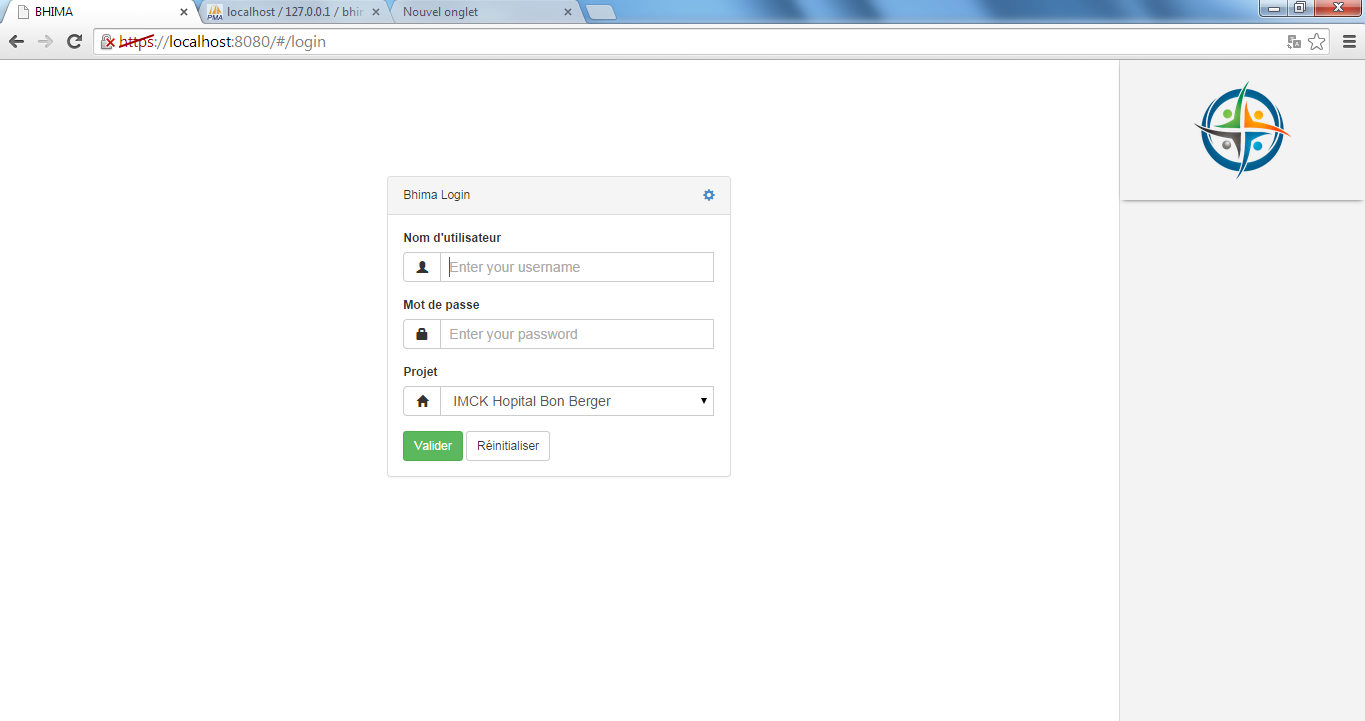
\includegraphics[width=12cm]{pic/login.png}
\end{center}
\caption{Page d'identification et authentification des utilisateurs}
\label{Page d'identification et authentification des utilisateurs}
\end{figure}
\\ L'accès au système n'est garanti que pour ceux qui possèdent un compte utilisateur, si l'utilisateur s'est authentifié alors il sera dirigé vers l'interface principale de l'application qui se présente de la manière suivante.
\newpage
\begin{figure}[h]
\begin{center}
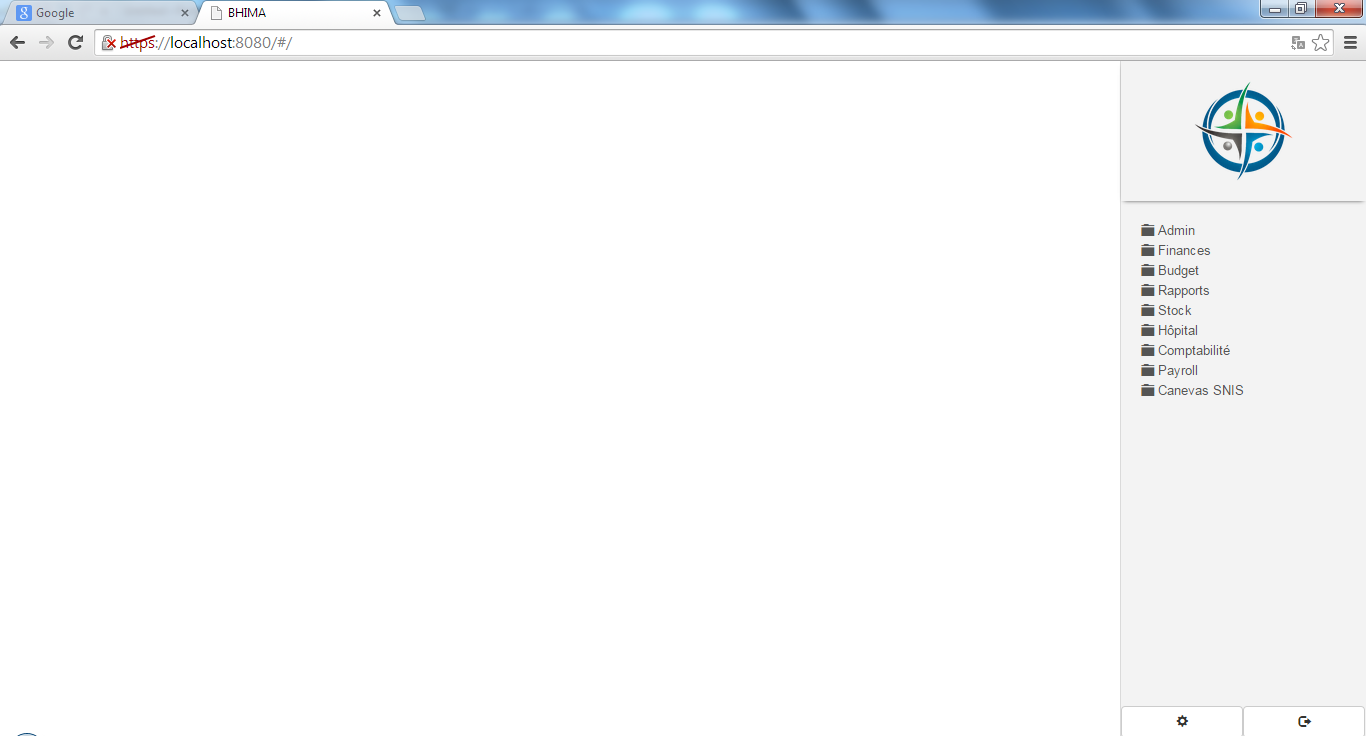
\includegraphics[width=10cm]{pic/mainInterface.png}
\end{center}
\caption{Interface principale de l'application}
\label{Interface principale de l'application}
\end{figure} 
Dans sa partie gauche de la figure ci-dessous on retrouve le logo IMA World Heath Ainsi que l'arborescence qui représente les modules du système auxquels l'utilisateur à accès. En dessous de l'arborescence figure deux boutons, le premier 
\includegraphics[scale=0.5]{pic/lang.png} permet de changer de langue et le second 
\includegraphics[scale=0.5]{pic/logout.png} permet de ce déconnecté du système.

\begin{figure}[h]
\begin{center}
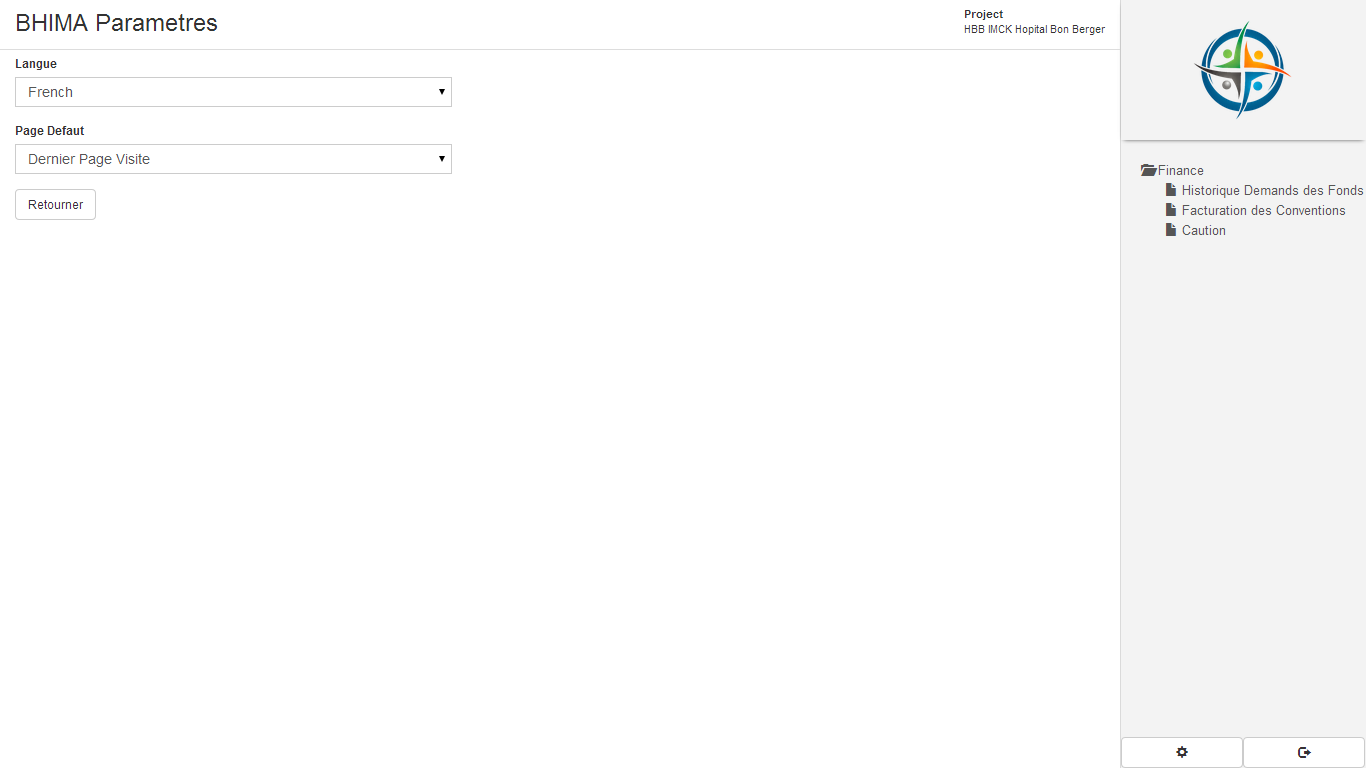
\includegraphics[width=10cm]{pic/changeLang.png}
\end{center}
\caption{Interface principale pour le changement de langue}
\label{Interface principale pour le changement de langue}
\end{figure} 
\newpage
\section{Les modules du système BHIMA}
Le système d'information BHIMA possède plusieurs modules qui sont représenté par l'arborescence ci-dessous.
\begin{figure}[h]
\begin{center}
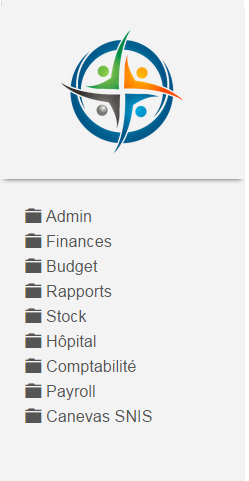
\includegraphics[width=4.5cm]{pic/arbo.png}
\end{center}
\caption{Arborescence du système}
\label{Arborescence du système}
Voici les différentes rubriques qui existent dans le système:
\end{figure} 
% Liste des modules
\begin{itemize}
\item Admin. %•
\item Budget
\item Canevas SNIS
\item Comptabilité
\item Finances
\item Hôpital
\item Payroll
\item Rapports
\item Stock




\end{itemize}
Nous allons à présent détailler chacun d'entre eux.
\newpage
%%%%%%%%%%%%%%%%%%%%%%%%%%%%%%%%%%%%%%%%%%%%%
%   MODULES DU SYSTEMES                     %
%%%%%%%%%%%%%%%%%%%%%%%%%%%%%%%%%%%%%%%%%%%%%
    
\chapter{Le module Admin}        
%////////////////////////////////////////////////%
% MODULE ADMIN
Le module admin est composé des sous modules qui permettent d'administrer le système. La figure ci-dessous représente avec exactitude ce module avec ses différents sous éléments.
\begin{figure}[h]
\begin{center}
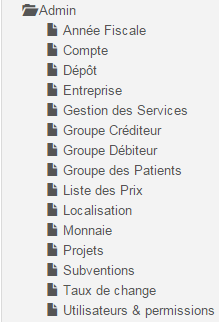
\includegraphics[width=4cm]{pic/s_admin.png}
\end{center}
\caption{Le module Admin et ses sous modules}
\label{Le module Admin et ses sous menus}
\end{figure} 

\section{Entreprise}
Le sous modules Entreprise permet d'ajouter une entreprise dans le système, ce module permet aussi de configurer certains paramètres nécessaire à une entreprise.

Son interface principale se présente de la manière suivante.

\begin{figure}[h]
\begin{center}
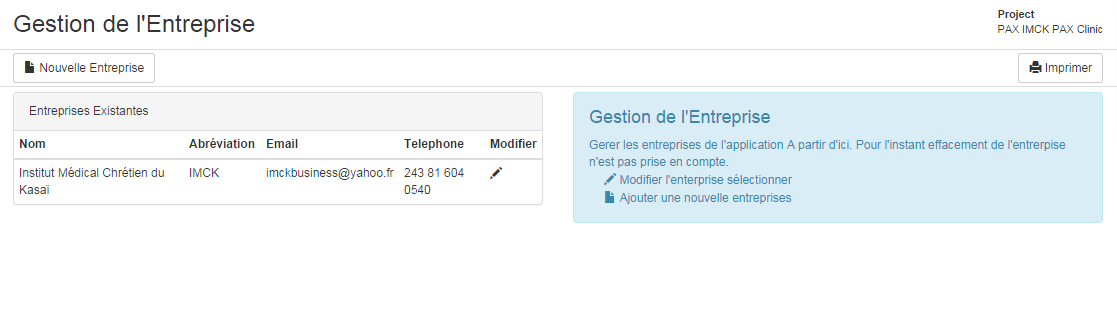
\includegraphics[width=14cm]{pic/ModuleEntreprise.png}
\end{center}
\caption{Interface principale du module entreprise}
\label{Interface principale du module entreprise}
\end{figure} 
\newpage
Dans la figure ci-haut on retrouve dans la partie gauche la liste des entreprises existante dans le système, au dessus de ce tableau il existe le bouton 
\includegraphics[scale=1]{pic/New_Entre.png} qui permet d'ajouter une nouvelle entreprise dans le système.

Le formulaire permettant l'ajouter une nouvelle entreprise dans le système se présente de la manière suivante.
\begin{figure}[h]
\begin{center}
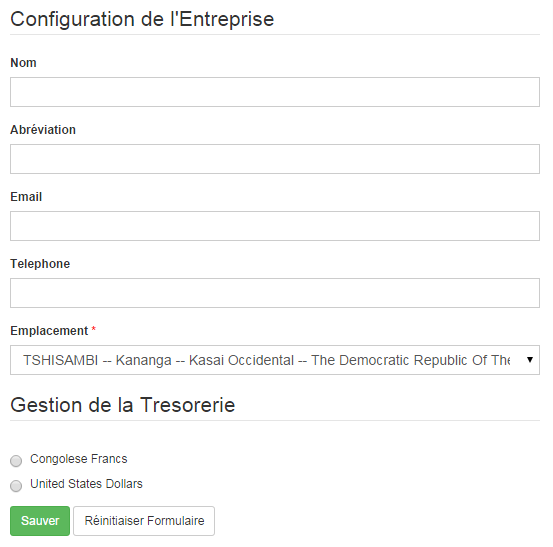
\includegraphics[width=8cm]{pic/Config_entreprise.png}
\end{center}
\caption{Interface de configuration d'une entreprise}
\label{Interface principale de la gestion des utilisateurs}
\end{figure} 

Une fois que tous ses éléments sont renseignés, il suffit de cliquer sur le bouton Sauver pour enregistrer une nouvelle entreprise et pour confirmer que l'entreprise qu'on vient d'ajouter est créér, il s'ajoutera automatiquement dans la liste des entreprises existantes. 

Les tableaux réprésentant les entreprises existante donne la possibilité de pouvoir mettre à jour les informations rélative à une entreprise. Le tableau comportant la liste des entreprises existantes comprend 5 rubriques, le Nom, l'abréviation, l'Email, le téléphone ainsi que la zone réservée a la modification, cette zone possède l'icône 
\includegraphics[scale=0.7]{pic/EditUser.png}, qui permet de modifier les méta données d'une entreprise, si l'on clique sur ce dernier un formulaire s'affiche dans la partie droite de l'ecran avec les informations rélatives à l'entreprise et avec la possibilité de pouvoir modifier si nécessaire et de valider les modifications grâce au bouton Sauver Changement.
\begin{figure}[h]
\begin{center}
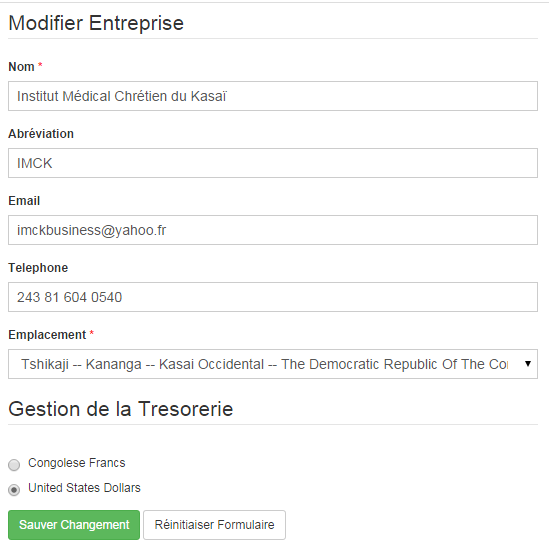
\includegraphics[width=8cm]{pic/ModEntreprise.png}
\end{center}
\caption{Apperçu du formulaire permettant la mise à jour des informations rélatives à une entreprise}
\label{Apperçu du formulaire permettant la mise à jour des informations rélatives à une entreprise}
\end{figure} 
\newpage
%/////////////% UTILISATEUR ET PERMISSION
\section{Utilisateur \& Permissions}
Le sous modules Utilisateur \& permissions d'ajouter des utilisateurs au système, d'administrer l'attributionde leur niveau d'accès, leur affiliation à des projets ainsi que l'administration du compte d'un utilisateur.

\begin{figure}[h]
\begin{center}
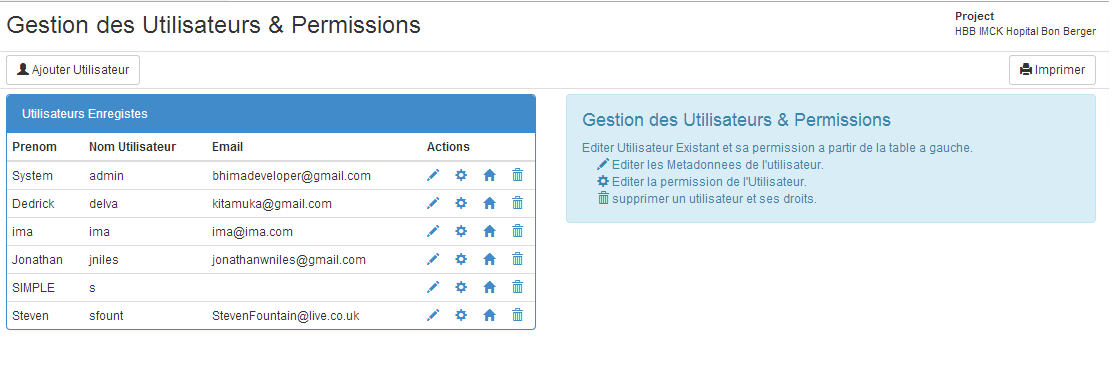
\includegraphics[width=14cm]{pic/userAllow.png}
\end{center}
\caption{Interface principale de la gestion des utilisateurs}
\label{Interface principale de la gestion des utilisateurs}
\end{figure} 
La figure ci haute résume à lui seule l'étendu de ce sous menu à savoir l'ajout d'un utilisateur. L'attribution de son niveau d'accès, son affiliation à un projet ainsi que la suppression du compte d'un utilisateur.

\subsection{Ajouter un utilisateur}
Lorsque l'utilisateur appuis sur le bouton 
\includegraphics[scale=1]{pic/AddUser.png}, le formulaire ci-après apparait.
\begin{figure}[h]
\begin{center}
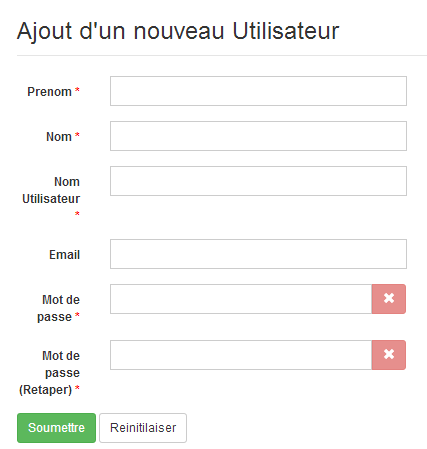
\includegraphics[width=8cm]{pic/FormAddUser.png}
\end{center}
\caption{Formulaire permettant d'ajouter un utilisateur}
\label{Formulaire permettant d'ajouter un utilisateur}
\end{figure}
\newpage
Après avoir rempli les différents champs de ce formulaire, la création n'est effective qu'après la validation du bouton Soumettre.
Une fois que le compte de l'utilisateur est créé, son compte s'ajoute dans la liste des comptes existant dans le système.

\subsection{Gestion des utilisateurs}
Pour gérer les utilisateurs du système, il suffit d'utiliser le tableau \textbf{Utilisateurs enregistrés}. Ce tableau compte 4 rubriques, le prénom, le nom de l'utilisateur son Email ainsi que la zone réservée aux actions, cette zone possède quatre icônes qui permet de modifier le compte de chaque utilisateur.
\begin{figure}[h]
\begin{center}
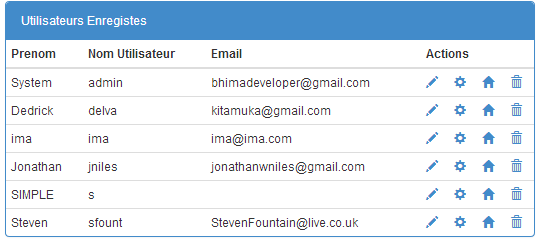
\includegraphics[width=12cm]{pic/ListUser.png}
\end{center}
\caption{Liste des utilisateurs enregistrés}
\label{Liste des utilisateurs enregistrés}
\end{figure}
\\
 
\includegraphics[scale=1]{pic/EditUser.png} Permet d'éditer les Métadonnées de l'utilisateur comme par exemple changer le nom de l'utilisateur, son login et même reinitialiser le mot de passe.
\\ 
 \begin{figure}[h]
\begin{center}
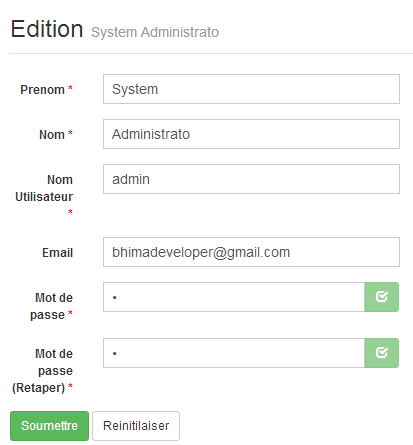
\includegraphics[width=6cm]{pic/UpdateUser.png}
\end{center}
\caption{Formulaire permettant de modifier les métadonnées d'un utilisateur}
\label{Formulaire permettant de modifier les métadonnées d'un utilisateur}
\end{figure}

\newpage
 
\includegraphics[scale=1]{pic/PermissionUser.png} Permet d'éditer la permission de l'Utilisateur.
 \begin{figure}[h]
\begin{center}
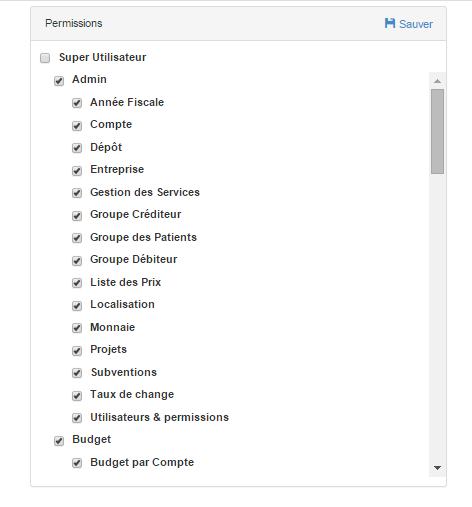
\includegraphics[width=6cm]{pic/ListeDePermission.png}
\end{center}
\caption{Aperçu de la liste de permission}
\label{Aperçu de la liste de permission}
\end{figure}
\\
La liste des permissions correspond exactement à la liste des fonctionnalités du système hormis le niveau d'accès super user qui permet d'accéder a toutes les fonctionnalités du système. Pour attribuer une permission à un utilisateur il suffit de cocher la dite permission.
\\
\\

\includegraphics[scale=1]{pic/Projet.png} Permet d'affilier l'utilisateur dans projets.
\begin{figure}[h]
\begin{center}
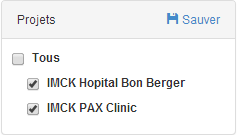
\includegraphics[width=6cm]{pic/ListeProjet.png}
\end{center}
\caption{Formulaire permettant de modifier l'attribution à des projets}
\label{Formulaire permettant de modifier l'attribution à des projets}
\end{figure}
Grâce à ce formulaire ont peux modifier l'attribution d'un utilisateur par rapport aux projets.
\newpage

\includegraphics[scale=1]{pic/DeleteUser.png} Permet de supprimer un compte utilisateur.
%//////////////////% 


\section{Comptes}
La figure ci-dessous représente l'interface principale permettant d'avoir des informations sur des comptes, de visualisation  leurs relations ainsi que la possibilité d'ajout d'un compte.

\begin{figure}[h]
\begin{center}
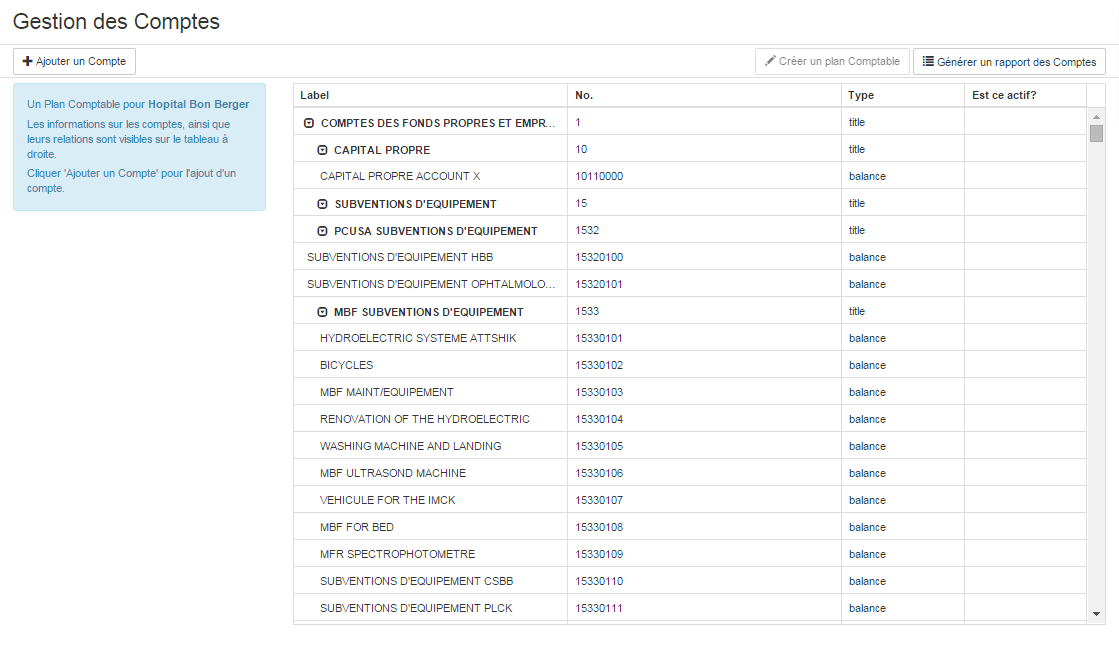
\includegraphics[width=13cm]{pic/GestionCompte.png}
\end{center}
\caption{Interface principale du module Gestion des comptes}
\label{Interface principale du module Gestion des comptes}
\end{figure}

\subsection{Ajout d'un compte}
Lorsque l'utilisateur click sur le bouton 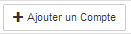
\includegraphics[scale=1]{pic/AjouterCompte.png} Le formulaire ci-après apparait.

\begin{figure}[h]
\begin{center}
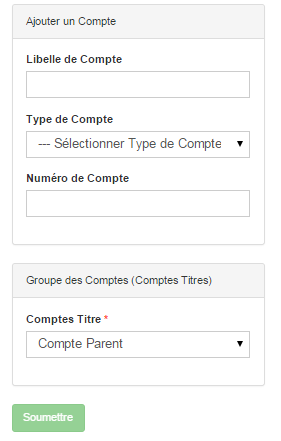
\includegraphics[width=4.5cm]{pic/FormAddCompte.png}
\end{center}
\caption{Formulaire permettant d'ajouter un compte}
\label{Formulaire permettant d'ajouter un compte}
\end{figure}

\begin{itemize}
\item \textbf{Le libelle de compte}: permet de nomme un compte \\
\item \textbf{Le type de Compte}: permet de dire si un compte est du type incom/expense, balance, title.\\
\item \textbf{Numero de compte}: permet de donner un numéro à un compte \\
\item \textbf{Groupe de comptes (Comptes titres)}: permet d'affilier un compte à un groupe de compte.\\
\end{itemize}

Si le compte est du type \textbf{Title}, un groupe de bouton radio apparait pour permettre de sélectionner dans quelle categorie des titres se trouve le compte, un compte de type title peut être soit \textbf{un actif}, \textbf{un passif} ou bien dans une autre catégorie.

Après avoir renseigner tous ce champ, un clic sur le bouton soumettre permet d'ajouter un compte dans la liste des comptes.
 
\subsection{Création d'un plan comptable}
Grace au bouton 
\includegraphics[scale=0.7]{pic/CreePlanCompt.png}, l'utilisateur peut créer un plan comptable pour l'entreprise ou bien pour l'organisation. \\

Après la création du plan comptable, ainsi que l'ajout de compte, le plan comptable apparait sous forme d'un tableau, dont les principaux entêtes sont :
\begin{itemize}
\item Texte
\item No
\item Type
\item Fixe
\item Editer
\item Effacer
\end{itemize}

Dans l'entête Texte on retrouve les noms des différents comptes ainsi que ceux de groupe de comptes, dans l'entête No on retrouve le différent numéro des comptes, l'entête Type permet de savoir si le compte est un Income /expence, Balance ou bien un titre et l'entête effacer permet de supprimé un compte.  Il y a aussi le bouton 
\includegraphics[scale=0.7]{pic/GenereRapportCompt.png} qui permet d'afficher une version imprimable du plan comptable.

Comme nous le montre l'image ci-après, on affiche le plan comptable de l'organisation par rapport à une date bien précise.\\

\begin{figure}[h]
\begin{center}
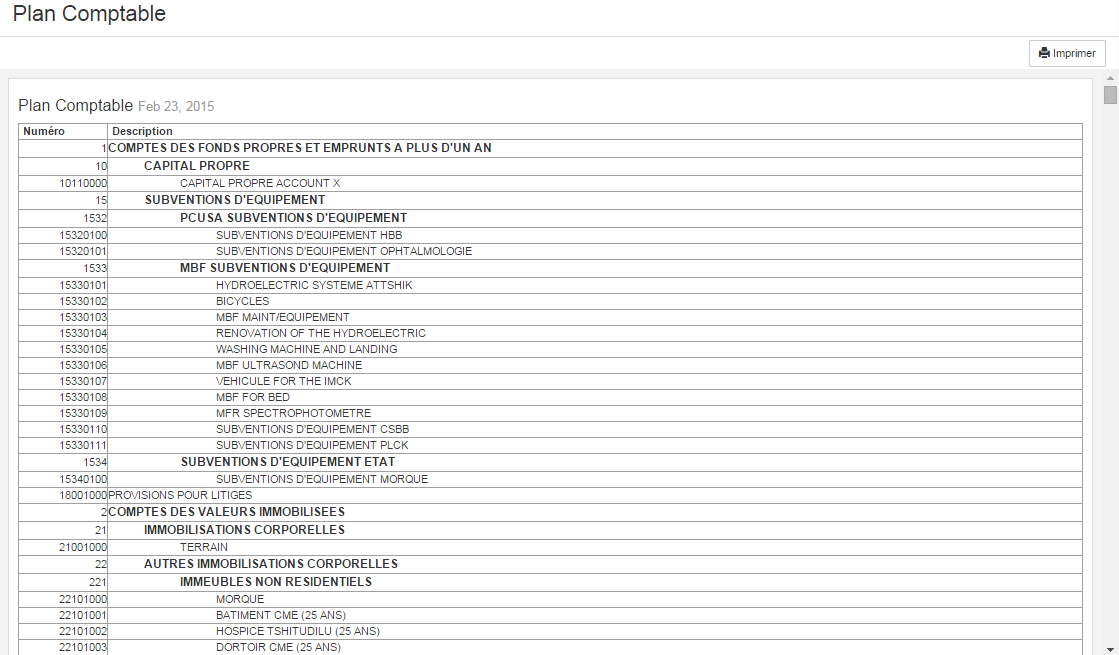
\includegraphics[width=14cm]{pic/PlanComptable.png}
\end{center}
\caption{Aperçue du plan Comptable}
\label{Aperçue du plan Comptable}
\end{figure}

Dans le coin supérieur droit existe le bouton \textbf{imprimer} qui permet d'imprimer le plan comptable.
\section{Année Fiscale}
La figure ci-dessous représente l'interface principale permettant la Gestion des années fiscales. 
\begin{figure}[h]
\begin{center}
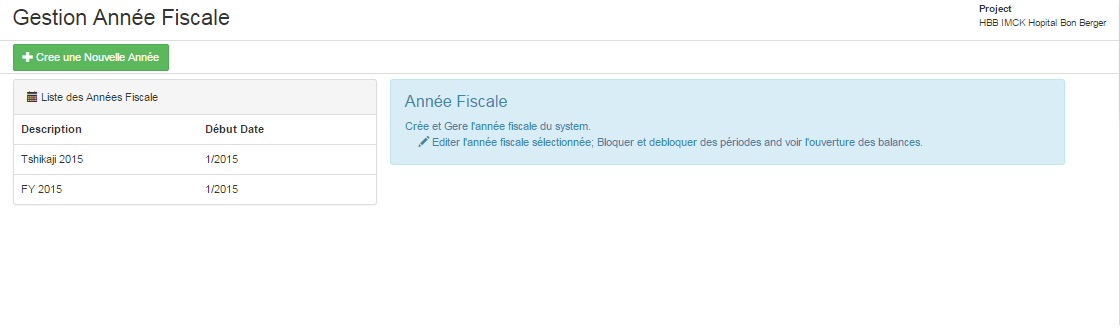
\includegraphics[width=14cm]{pic/AnneeFiscal.png}
\end{center}
\caption{Interface permettant de gérer les années fiscals}
\label{Interface permettant de gérer les années fiscals}
\end{figure}

\newpage
\subsection{Création de l'année fiscale}
Lorsque l'utilisateur click sur le bouton 
\includegraphics[scale=0.7]{pic/CreeAnnFisc.png} Le formulaire ci-après apparait.

\begin{figure}[h]
\begin{center}
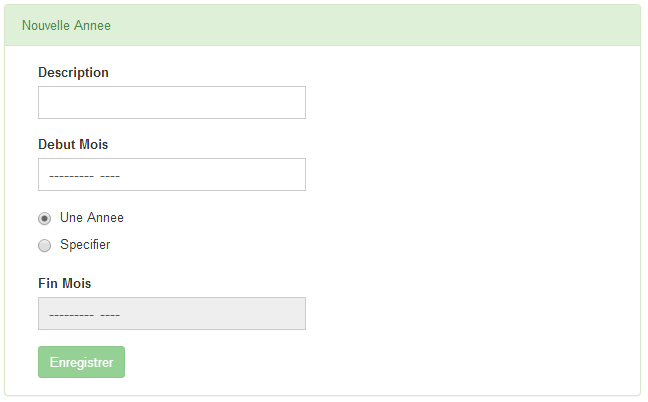
\includegraphics[width=12cm]{pic/FormCreationAnnFisc.png}
\end{center}
\caption{Formulaire d'ajouter une année fiscale}
\label{Formulaire d'ajouter une année fiscale}
\end{figure}
\begin{itemize}
\item \textbf{Description}: permet de décrire l'année fiscale.
\item \textbf{Début Mois}: permet de préciser le premier mois de l'année fiscale
\end{itemize}
\textbf{Il existe aussi deux boutons radio une année et Spécifier }: si l'on clique sur le bouton radio \textbf{une année}, l'année fiscale commencera à partir de la période préciser et couvrira une période de douze mois mais si l'on clique sur le bouton \textbf{spécifier} dans ce cas l'utilisateur devra préciser le champ \textbf{Fin Mois} qui marquera la fin de l'année fiscale.

Le champ \textbf{Année Fiscale précédent} n'apparait que s'il existe au moins une année fiscale déjà enregistrer dans le système. 

Après avoir renseigné tous ce champ, un clic sur le bouton \textbf{Enregistrer} redirige vers la deuxième étape de la création d'année fiscale qu'au cas ou il existait une année fiscale précédente à celle qui est en train d'être créer. Cette interface permet juste la confirmation de la fermeture de l'année fiscale précédente.

\begin{figure}[h]
\begin{center}
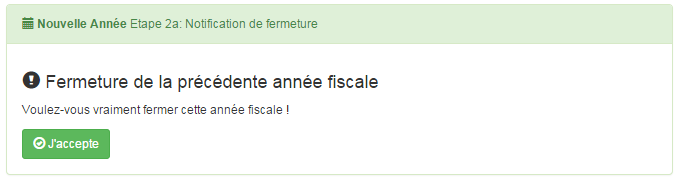
\includegraphics[width=12cm]{pic/CloseFiscYear.png}
\end{center}
\caption{Aperçue de l'interface permettant la fermeture de l'année fiscale précédente}
\label{Aperçue de l'interface permettant la fermeture de l'année fiscale précédente}
\end{figure}

La troisième étape de la création d'une année fiscale n'est juste qu'une interface de confirmation de la fermeture de l'année fiscale, cette troisième étape devient la deuxième étape de la création d'une année fiscale dans le cas ou il n'existait pas encore d'autres années fiscale.

\begin{figure}[h]
\begin{center}
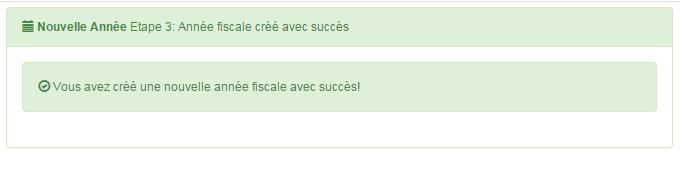
\includegraphics[width=12cm]{pic/ConfirSucces.png}
\end{center}
\caption{Message de confirmation de la création de la nouvelle année fiscale}
\label{Message de confirmation de la création de la nouvelle année fiscale}
\end{figure}

\newpage

\subsection{Liste des années fiscale}
Voici comment se présente la liste des années fiscale

\begin{figure}[h]
\begin{center}
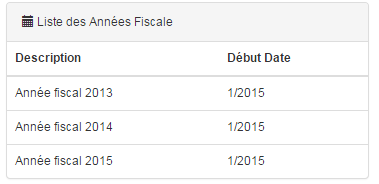
\includegraphics[width=9cm]{pic/ListeAnnFisc.png}
\end{center}
\caption{Aperçue de la liste des années fiscales}
\label{Aperçue de la liste des années fiscaux}
\end{figure}

Pour pouvoir visualiser les détailles d'une année fiscale il suffit de cliquer sur cette année fiscale dans la liste des années fiscaux.

\begin{figure}[h]
\begin{center}
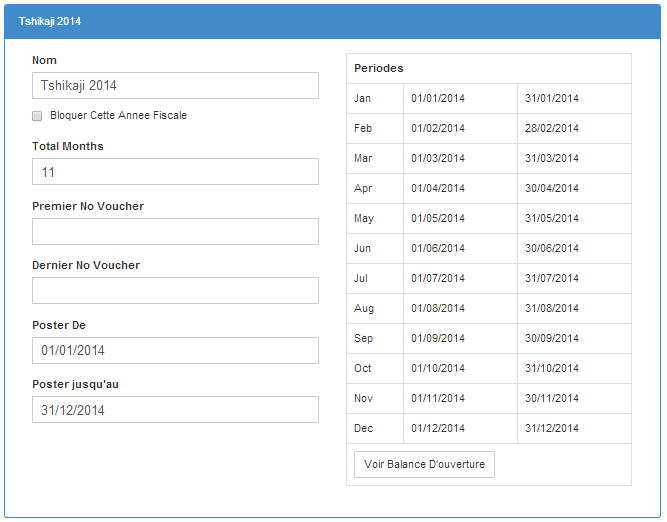
\includegraphics[width=12cm]{pic/FormAddFiscYear.png}
\end{center}
\caption{Interface principale de management d'une année fiscal}
\label{Interface principale de management d'une année fiscal}
\end{figure}

Dans la partie gauche de l'image ci-haut on retrouve la liste des années fiscales, on peut aussi , modifier la designation d'une année fiscale, visualiser les différentes périodes qui constituent cette année fiscale. 

\newpage
\section{Liste des prix}
La figure ci-dessous représente l'interface principale permettant la Gestion de la liste des prix. 
\begin{figure}[h]
\begin{center}
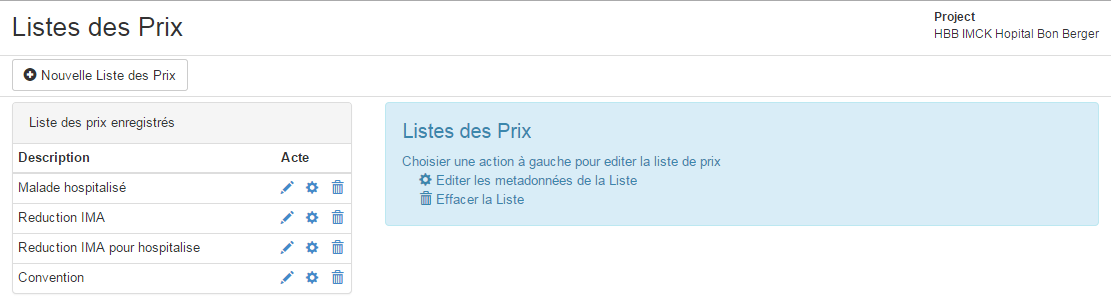
\includegraphics[width=12cm]{pic/ListePrix.png}
\end{center}
\caption{Interface permettant de faire la gestion des prix}
\label{Interface permettant de faire la gestion des prix}
\end{figure}

\subsection{Nouvelle liste des prix}
Lorsque l'utilisateur click sur le bouton 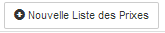
\includegraphics[scale=0.7]{pic/NewListePrix.png} Le formulaire ci-après apparait.

\begin{figure}[h]
\begin{center}
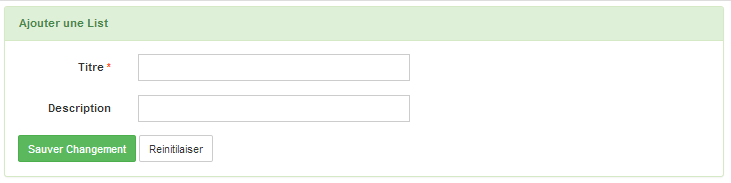
\includegraphics[width=14cm]{pic/AjouterListePrix.png}
\end{center}
\caption{Formulaire permettant d'ajouter un élément dans la liste des prix}
\label{Formulaire permettant d'ajouter un élément dans la liste des prix}
\end{figure}

\textbf{Titre}: permet de décrire la catégorie que l'on veut ajouter à la liste des prix.
\textbf{Description}: permet de données des informations supplémentaires au nouvel élément de la liste des prix. 
Après avoir renseigné tous ce champ, un clic sur le bouton \textbf{Sauver changement} permet d'ajouter un nouvel élément dans ladite liste.

\subsection{Liste des prix enregistré}

La liste des prix enregistrés possède deux entêtes \textbf{Description} et \textbf{Acte}, pour chaque élément de la liste existe l'icône 
\includegraphics[scale=0.7]{pic/EditBlack.png}  qui permet de mettre à jour les informations relatives à ce dernier. Il y'a aussi un autre icône  
\includegraphics[scale=0.7]{pic/UpdateBlack.png} qui permet d'éditer les métadonnées de la liste et le dernier icône 
\includegraphics[scale=0.7]{pic/DeleteRed.png}  permet d'effacer une liste de prix.

Lorsqu'on clique sur l'icône qui permet de mettre à jour les informations relatives à la liste de prix le formulaire qui apparait ressemble à celui utilisé pour l'ajout d'un élément dans la liste de prix sauf que cette fois ci il permet de faire l'opération des mis à jour.
Dans l'image ci-après est illustré le formulaire utilisé pour le mis à jour.

\begin{figure}[h]
\begin{center}
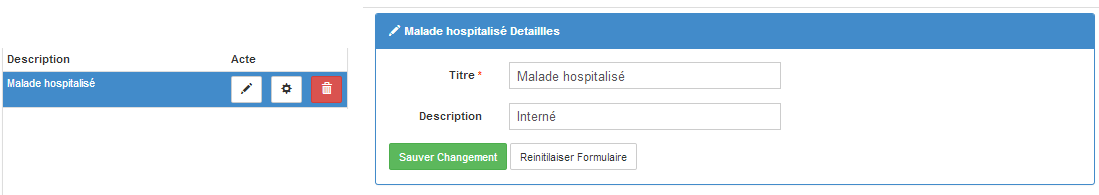
\includegraphics[width=14cm]{pic/FormUpdateListePrice.png}
\end{center}
\caption{Formulaire permettant de mettre à jour un élément de la liste des prix}
\label{Formulaire permettant de mettre à jour un élément de la liste des prix}
\end{figure}

L'édition des métadonnées des éléments d'une liste est très important car ce grâce à ces informations qu'on peut distinguer un élément de la liste de prix à un autre.

Le formulaire d'édition de métadonnées ce présente comme suit.

\begin{figure}[h]
\begin{center}
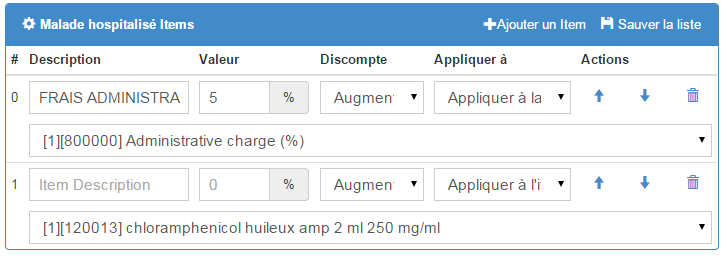
\includegraphics[width=14cm]{pic/EditionMetaDonneListeP.png}
\end{center}
\caption{Formulaire d'édition de Metadonnées d'un élément de la liste des prix}
\label{Formulaire permettant de mettre à jour un élément de la liste de prix}
\end{figure}

Dans l'entête à gauche est repris le nom de la liste de prix et à droite il y'a un bouton qui permet d'ajouter un item pour les particularités de ladite liste initialement il existe un autre bouton Sauver la liste qui se retrouve à côté de celui-ci.

En dessous de l'entête se trouve les divers champs qui permet d'enrichir un item en premier il y'a \textbf{Item Description} qui permet de décrire un item, en second lieu il y'a \textbf{Valeur} qui s'exprime en Pourcentage par rapport au prix du bien ou service consommé par le patient, Discompte permet de déterminer l'action à effectuer aux pourcentage qui a était fourni dans le champ valeur dans la liste de choix du champ Discompte il y'a \textbf{l'augmentation et la diminution}, \textbf{Appliquer à} permet de déterminer si les informations fourni   aux champs Valeur et discompte s'appliquera à un item ou bien à la facture, en dessous de cette zone de configuration on retrouve une liste de choix qui permet de sélection le item qui fera partie de la liste de prix. L'entête Actions possède une série d'icône dont le deux premiers permet de modifier l'ordre d'affichage des éléments d'une liste « seule pour les listes des prix qui possède plusieurs item », le dernier icône permet de supprimer un item de la liste de prix.
\newpage
\section{Taux d'échange}
Le module de taux de change, donne la possibilité de définir le taux d'échange du jour. Par souci d'intégrité des données, Le taux d'échange doit être défini chaque jour.


\begin{figure}[h]
\begin{center}
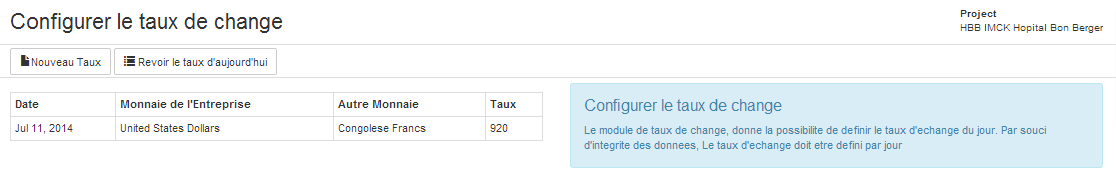
\includegraphics[width=16cm]{pic/FormulaireConfigRate.png}
\end{center}
\caption{Formulaire permettant de configurer le taux de change}
\label{Formulaire permettant de configurer le taux de change}
\end{figure}

\subsection{Nouveau Taux}
Lorsque l'utilisateur click sur le bouton 
\includegraphics[scale=0.7]{pic/NouveauTaux.png}
 Le formulaire ci-après apparait.

\begin{figure}[h]
\begin{center}
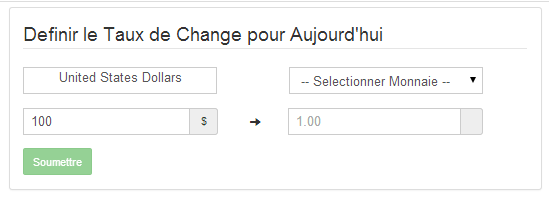
\includegraphics[width=12cm]{pic/DefinirTaux.png}
\end{center}
\caption{Formulaire permettant de definir le taux}
\label{Formulaire permettant de definir le taux}
\end{figure}
\begin{itemize}
\item \textbf{United States Dollars}: est la monnaie principale de l'application, l'équivalence avec d'autres monnaies ne doit se faire qu'avec la somme de 100 Dollars,
\item \textbf{Sélectionner Monnaie}: Affiche la liste des monnaies qui existe dans le système et la zone de saisie qui se retrouve en bas permet de préciser l'équivalence avec la monnaie principale.
\end{itemize}
Après avoir renseigné ce deux champs, un clique sur le bouton \textbf{Soumettre} permet de définir les taux du jour.

\subsection{Revoir le taux d'aujourd'hui}
Un clic sur le bouton 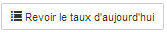
\includegraphics[scale=0.7]{pic/RevoirTaux.png} permet d'afficher toutes les informations sur le taux du jour, comme la montre la figure ci-dessous.
\begin{figure}[h]
\begin{center}
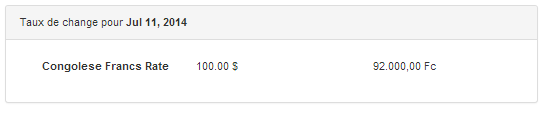
\includegraphics[width=12cm]{pic/ShowRate.png}
\end{center}
\caption{Aperçue du taux du jour}
\label{Aperçue du taux du jour}
\end{figure}
\newpage
\section{Groupe Créditeur}
Ce module permet de faire la gestion des groupes créditeurs, l'interface principale de ce module se présente de la manière que voici.

\begin{figure}[h]
\begin{center}
\includegraphics[width=12cm]{pic/AdminGroupCredit.png}
\end{center}
\caption{Interface principale permettant d'administrer le groupe créditeur}
\label{Interface principale permettant d'administrer le groupe créditeur}
\end{figure}


Le bouton \includegraphics[scale=0.7]{pic/NewGroupCredit.png} permet d'ajouter un nouveau groupe créditeur dans ladite liste.

\begin{figure}[h]
\begin{center}
\includegraphics[width=12cm]{pic/AddNewGroupCred.png}
\end{center}
\caption{Ajouter un nouveau groupe créditeur}
\label{Ajouter un nouveau groupe créditeur}
\end{figure}

Le formulaire ci-haut apparait lorsqu'un utilisateur clique sur le bouton \textbf{Nouveau groupe Créditeur}. Ce formulaire possède deux champs, le premier \textbf{Nom du groupe} permet de spécifier le nom du groupe et \textbf{Numéro de compte}  le numéro de compte permet de choisir dans la liste de compte, celui correspondant au groupe créditeur.
L'enregistrement est effectif seulement si l'utilisateur clique sur le bouton Sauver changement.
La liste des groupes créditeurs apparait sous forme de tableau. Ce tableau possède quatre rubriques. Le premier \textbf{Nom du groupe} renseigne sur le nom du groupe, le second renseigne sur le numéro de compte, en troisième lieu il y'a une rubrique qui est représenté par l'icône \includegraphics[scale=0.7]{pic/Locked.png}  qui permet de verrouiller mais aussi de déverrouillé un groupe créditeur à l'aide de case à coché et denier lieu il y'a \textbf{Editer} qui contient l'icône  \includegraphics[scale=0.7]{pic/EditUser.png} permet de modifier les informations sur un groupe créditeur.

\section{Groupe Débiteur}
Ce module permet de faire l'administration de groupe débiteur, l'interface principale de ce module se présente de la manière que voici.

\begin{figure}[h]
\begin{center}
\includegraphics[width=14cm]{pic/AdminGroupDebit.png}
\end{center}
\caption{Interface principale permettant d'administrer le groupe débiteur}
\label{Interface principale permettant d'administrer le groupe débiteur}
\end{figure}

Le bouton \includegraphics[scale=0.7]{pic/NewGroupDebit.png} permet d'ajouter un nouveau groupe Débiteur dans ladite liste.
\newpage
\begin{figure}[h]
\begin{center}
\includegraphics[width=9cm]{pic/FormAddGroupDebiteur.png}
\end{center}
\caption{Formulaire permettant d'ajouter un groupe débiteur}
\label{Formulaire permettant d'ajouter un groupe débiteur}
\end{figure}

Le formulaire ci-haut apparait lorsqu'un utilisateur clique sur le bouton \textbf{Nouveau groupe Débiteur}. Ce formulaire possède dix champs, le premier \textbf{Nom} permet de spécifier le nom du groupe débiteur, ensuite il existe une case à coché convention qui permet de déterminer si le groupe débiteur est une convention ou nom, \textbf{Compte }permet d'attribuer un compte, \textbf{Liste de prix}  permet de spécifier pour quelle liste de prix fait référence un groupe débiteur, \textbf{Localisation} permet de spécifier l'emplacement géographique relative à un groupe de compte, \textbf{Paiement} permet de spécifier le type de paiement relative à un groupe,\textbf{ Phone}, \textbf{Email}, \textbf{Crédit Max }et \textbf{Note} sont d'autres informations qu'on peut attribuer à un groupe débiteur.
L'enregistrement est effectif seulement si l'utilisateur clique sur le bouton Sauver changement.
La liste des groupes débiteurs apparait sous forme de tableau. Ce tableau possède cinq rubriques, il y'a Nom, Compte, Convention qui est soit vide ou bien représenté par l'icône \includegraphics[scale=0.7]{pic/IconOk.png}  seulement si le groupe débiteur appartient à un groupe de conventionné,  il y'a aussi l'icône \includegraphics[scale=0.7]{pic/Locked.png}  qui permet de verrouiller mais aussi de déverrouillé un groupe débiteur à l'aide de case à coché et denier lieu il y'a \textbf{Editer} qui contient l'icône \includegraphics[scale=0.7]{pic/EditUser.png}   permet de modifier les informations sur un groupe débiteur.

\newpage
\section{Localisation}
Gestions Emplacement permet d'enregistrer toutes les localisations possible pour l'enregistrement des patients. L'interface principale se présente comme de la manière suivante.

\begin{figure}[h]
\begin{center}
\includegraphics[width=14cm]{pic/AdminLocalisation.png}
\end{center}
\caption{Interface principale du module gestion des emplacement}
\label{Interface principale du module gestion des emplacement}
\end{figure}

Dans la partie droite l'on trouve le bouton qui permet d'ajouter les différents niveaux d'emplacement en commençant par la gestion des villages, des secteurs, des provinces ainsi que celui des pays. En dessous de ce menu de configuration est affiché sur un tableau les différents emplacements qui ont étaient enregistrés dans ce système. 
\newpage
\subsection{Gestion des villages}
Pour faire l'administration des villages, il suffit de cliquer sur le bouton\\ \includegraphics[scale=0.7]{pic/GererVillage.png}, ceci redirige vers la page qui permet une telle administration.

\begin{figure}[h]
\begin{center}
\includegraphics[width=14cm]{pic/AdminVillage.png}
\end{center}
\caption{Interface principale permettant d'administrer les villages}
\label{Interface principale permettant d'administrer les villages}
\end{figure}

Le bouton \includegraphics[scale=0.7]{pic/GestionEmplacement.png} redirige vers la page principale de la gestion des emplacements.

Le bouton \includegraphics[scale=0.7]{pic/AddVillage.png} permet d'ajouter un village dans ladite liste.

\begin{figure}[h]
\begin{center}
\includegraphics[width=14cm]{pic/FormAddVillage.png}
\end{center}
\caption{Formulaire permettant d'ajouter un village}
\label{Formulaire permettant d'ajouter un village}
\end{figure}

Le formulaire ci-haut apparait lorsqu'un utilisateur clique sur le bouton \textbf{ajouter village}. Ce formulaire possède deux champs, le premier \textbf{commune} renferme la liste de toutes les communes enregistré dans le système. 
L'enregistrement est effectif seulement si l'utilisateur clique sur le bouton soumettre. La liste des villages apparait sous forme de tableau. Ce tableau a trois rubriques. Le premier \textbf{Nom} renseigne sur le nom du village, le second \textbf{Commune} permet de savoir dans quelle commune se trouve le village et le dernier \textbf{Actions} renferme deux icônes le premier \includegraphics[scale=0.7]{pic/EditUser.png}  permet de modifier les informations sur un village et le second \includegraphics[scale=0.7]{pic/DeleteWRed.png}  permet de supprimer un village.

\subsection{Gérer les secteurs}
Pour faire l'administration des secteurs, il suffit de cliquer sur le bouton \includegraphics[scale=0.7]{pic/AdminSecteur.png} pour être redirigé vers la page qui permet une telle administration.

\begin{figure}[h]
\begin{center}
\includegraphics[width=12cm]{pic/FormulaireGestionSecteur.png}
\end{center}
\caption{Aperçue de l'interface permettant la gestion des secteurs}
\label{Aperçue de l'interface permettant la gestion des secteurs}
\end{figure}

Le bouton \includegraphics[scale=0.7]{pic/GestionEmplacement.png} redirige vers la page principale de la gestion des emplacements.
Le bouton \includegraphics[scale=0.7]{pic/AddSecteur.png} permet d'ajouter un secteur dans ladite liste.

\begin{figure}[h]
\begin{center}
\includegraphics[width=10cm]{pic/FormAddSecteur.png}
\end{center}
\caption{Formulaire permettant d'ajouter les secteurs}
\label{Formulaire permettant d'ajouter les secteurs}
\end{figure}

Le formulaire ci-haut apparait lorsqu'un utilisateur clique sur le bouton \textbf{ajouter secteur}. Ce formulaire possède deux champs, le premier \textbf{Province} renferme la liste de toutes les provinces enregistré dans le système. 
L'enregistrement est effectif seulement si l'utilisateur clique sur le bouton Ajouter. La liste des secteurs apparait sous forme de tableau. Ce tableau a trois rubriques. Le premier\textbf{ Nom} renseigne sur le nom du secteur, le second \textbf{Province} permet de savoir dans quelle commune se trouve le village et le dernier \textbf{Actions} renferme deux icônes le premier 
\includegraphics[scale=0.7]{pic/EditUser.png}  permet de modifier les informations sur un secteur et le second 
 \includegraphics[scale=0.7]{pic/DeleteWRed.png}  permet de supprimer un secteur.
\subsection{Gérer les provinces}
Pour faire l'administration des provinces, il suffit de cliquer sur le bouton \includegraphics[scale=0.7]{pic/AdminProvince.png} pour être redigé vers la page qui permet une telle administration.
\begin{figure}[h]
\begin{center}
\includegraphics[width=14cm]{pic/InterfaceGestionProvince.png}
\end{center}
\caption{Interface principale permettant la gestion des provinces}
\label{Interface principale permettant la gestion des provinces}
\end{figure}

Le bouton \includegraphics[scale=0.7]{pic/GestionEmplacement.png} redirige vers la page principale de la gestion des emplacements.

Le bouton \includegraphics[scale=0.7]{pic/AddNewProvince.png} permet d'ajouter une province dans ladite liste.
\begin{figure}[h]
\begin{center}
\includegraphics[width=10cm]{pic/FormNewProvince.png}
\end{center}
\caption{Formulaire permettant d'ajouter une province}
\label{Formulaire permettant d'ajouter une province}
\end{figure}


Le formulaire ci-haut apparait lorsqu'un utilisateur clique sur le bouton ajouter province. Ce formulaire possède deux champs, le premier Pays renferme la liste de tous les pays. 
L'enregistrement est effectif seulement si l'utilisateur clique sur le bouton Ajouter. La liste des provinces apparait sous forme de tableau. Ce tableau a trois rubriques. Le premier \textbf{Nom} renseigne sur le nom de la province, le second \textbf{Pays} permet de savoir dans quelle pays se trouve une province et le dernier \textbf{Actions} renferme deux icônes le premier 
\includegraphics[scale=0.7]{pic/EditUser.png}  permet de modifier les informations sur une province et le second  \includegraphics[scale=0.7]{pic/DeleteWRed.png}  permet de supprimer une province.
\subsection{Gérer les pays}
Pour faire l'administration des pays, il suffit de cliquer sur le bouton \includegraphics[scale=0.7]{pic/AddNewCountry.png}, ceci redirige vers la page qui permet une telle administration.
\begin{figure}[h]
\begin{center}
\includegraphics[width=14cm]{pic/AdminCountry.png}
\end{center}
\caption{Interface principale permettant la gestion des pays}
\label{Interface principale permettant la gestion des pays}
\end{figure}

Le bouton \includegraphics[scale=0.7]{pic/GestionEmplacement.png}  permet redirige vers la page principale de la gestion des emplacements.

Le bouton \includegraphics[scale=0.7]{pic/AddCountry.png} permet d'ajouter un pays dans ladite liste.

\begin{figure}[h]
\begin{center}
\includegraphics[width=10cm]{pic/SaveCountry.png}
\end{center}
\caption{Enregistrer un pays}
\label{Enregistrer un pays}
\end{figure}

Le formulaire ci-haut apparait lorsqu'un utilisateur clique sur le bouton \textbf{ajouter Nouveau pays}. Ce formulaire possède trois champs, le premier \textbf{Code} permet de donner un code à un pays ensuite un champ pour donner le nom du pays en \textbf{Anglais} et l'autre pour le \textbf{Français}.
L'enregistrement est effectif seulement si l'utilisateur clique sur le bouton Ajouter. La liste des pays apparait sous forme de tableau. Ce tableau a trois rubriques. Le premier \textbf{Code} renseigne sur le code qui a été attribué au pays, le second \textbf{Nom en anglais} suivi de \textbf{Nom}  et le dernier \textbf{Actions} renferme deux icônes le premier \includegraphics[scale=0.7]{pic/EditUser.png}  permet de modifier les informations sur un pays et le second \includegraphics[scale=0.7]{pic/DeleteWRed.png}  permet de supprimer un pays.


\section{Subventions}
La figure ci-dessous représente l'interface principale permettant la Gestion des subventions. 
\begin{figure}[h]
\begin{center}
\includegraphics[width=12cm]{pic/MainSubvention.png}
\end{center}
\caption{Interface permettant l'administration des subventions}
\label{Interface permettant l'administration des subventions}
\end{figure}

Dans la figure ci-haute on retrouve dans la partie gauche la liste des différents subventions enregistrées dans le système, au dessus de ce tableau existe le bouton \includegraphics[scale=1]{pic/NewSubvention.png} qui permet d'ajouter un nouveau grade dans le système, le formulaire permettant d'enregistrer une nouvelle subvention se présente de la manière suivante.

\begin{figure}[h]
\begin{center}
\includegraphics[width=8cm]{pic/FormSubvention.png}
\end{center}
\caption{Formulaire permettant l'enregistrement des subventions}
\label{Formulaire permettant l'enregistrement des subventions}
\end{figure} 

Le formulaire permettant l'enregistrement des subventions comporte quatre zones de saisie rélative à la désignation de la subvention, le champ en pourcentage permet de spécifier si la subvention s'exprime en terme  de pourcentage, le champ valeur permet de renseigner la valeur de la subvention soit en pourcentage ou bien à l'unité monnetaire et le dernier permet de spécifier le débiteur qui prend en charge la subvention. 

Les tableaux réprésentant les subventions enregistrées donne la possibilité de pouvoir mettre à jour les informations rélative à une subventions, dans la zone action de ce tableau on retrouve deux icônes, l'icône \includegraphics[scale=0.7]{pic/EditBlack.png} qui permet de mettre à jour une subventions et \includegraphics[scale=0.7]{pic/DeleteWRed.png} permet de supprimer une subvention dans le système.
Voici un apperçu du formulaire permettant la mise à jour des informations d'une subvention, la mise à jour est effective que si l'on modifier les informations dont on a besoin en validant grace au bouton soumettre. 

\begin{figure}[h]
\begin{center}
\includegraphics[width=8cm]{pic/FormUpSubventions.png}
\end{center}
\caption{Formulaire permettant de mettre à jour les informations d'une subvention}
\label{Formulaire permettant de mettre à jour les informations d'une subvention}
\end{figure} 

\newpage
\section{Taux d'échange}
Le module de taux de change, donne la possibilité de définir le taux d'échange du jour. Par souci d'intégrité des données, Le taux d'échange doit être défini chaque jour.


\begin{figure}[h]
\begin{center}
\includegraphics[width=16cm]{pic/FormulaireConfigRate.png}
\end{center}
\caption{Formulaire permettant de configurer le taux de change}
\label{Formulaire permettant de configurer le taux de change}
\end{figure}

\subsection{Nouveau Taux}
Lorsque l'utilisateur click sur le bouton \includegraphics[scale=0.7]{pic/NouveauTaux.png}
 Le formulaire ci-après apparait.

\begin{figure}[h]
\begin{center}
\includegraphics[width=12cm]{pic/DefinirTaux.png}
\end{center}
\caption{Formulaire permettant de definir le taux}
\label{Formulaire permettant de definir le taux}
\end{figure}
\begin{itemize}
\item \textbf{United States Dollars}: est la monnaie principale de l'application, l'équivalence avec d'autres monnaies ne doit se faire qu'avec la somme de 100 Dollars,
\item \textbf{Sélectionner Monnaie}: Affiche la liste des monnaies qui existe dans le système et la zone de saisie qui se retrouve en bas permet de préciser l'équivalence avec la monnaie principale.
\end{itemize}
Après avoir renseigné ce deux champs, un clique sur le bouton \textbf{Soumettre} permet de définir les taux du jour.

\subsection{Revoir le taux d'aujourd'hui}
Un clic sur le bouton \includegraphics[scale=0.7]{pic/RevoirTaux.png} permet d'afficher toutes les informations sur le taux du jour, comme la montre la figure ci-dessous.
\begin{figure}[h]
\begin{center}
\includegraphics[width=12cm]{pic/ShowRate.png}
\end{center}
\caption{Aperçue du taux du jour}
\label{Aperçue du taux du jour}
\end{figure}
\newpage
\section{Groupe Créditeur}
Ce module permet de faire la gestion des groupes créditeurs, l'interface principale de ce module se présente de la manière que voici.

\begin{figure}[h]
\begin{center}
\includegraphics[width=12cm]{pic/AdminGroupCredit.png}
\end{center}
\caption{Interface principale permettant d'administrer le groupe créditeur}
\label{Interface principale permettant d'administrer le groupe créditeur}
\end{figure}


Le bouton \includegraphics[scale=0.7]{pic/NewGroupCredit.png} permet d'ajouter un nouveau groupe créditeur dans ladite liste.

\begin{figure}[h]
\begin{center}
\includegraphics[width=12cm]{pic/AddNewGroupCred.png}
\end{center}
\caption{Ajouter un nouveau groupe créditeur}
\label{Ajouter un nouveau groupe créditeur}
\end{figure}

Le formulaire ci-haut apparait lorsqu'un utilisateur clique sur le bouton \textbf{Nouveau groupe Créditeur}. Ce formulaire possède deux champs, le premier \textbf{Nom du groupe} permet de spécifier le nom du groupe et \textbf{Numéro de compte}  le numéro de compte permet de choisir dans la liste de compte, celui correspondant au groupe créditeur.
L'enregistrement est effectif seulement si l'utilisateur clique sur le bouton Sauver changement.
La liste des groupes créditeurs apparait sous forme de tableau. Ce tableau possède quatre rubriques. Le premier \textbf{Nom du groupe} renseigne sur le nom du groupe, le second renseigne sur le numéro de compte, en troisième lieu il y'a une rubrique qui est représenté par l'icône \includegraphics[scale=0.7]{pic/Locked.png}  qui permet de verrouiller mais aussi de déverrouillé un groupe créditeur à l'aide de case à coché et denier lieu il y'a \textbf{Editer} qui contient l'icône  \includegraphics[scale=0.7]{pic/EditUser.png} permet de modifier les informations sur un groupe créditeur.


\newpage
\section{Groupe des Patients}
Ce menu permet d'enregistrer toutes les groupes permettant des catégorisés les différents type des patients. Qui sont admis au sein de l'hôpital. 
L'interface principale se présente comme de la manière suivante.

\begin{figure}[h]
\begin{center}
\includegraphics[width=16cm]{pic/AdminGroupPatient.png}
\end{center}
\caption{Interface principale de la gestion des groupes des malades}
\label{Interface principale de la gestion des groupes des malades}
\end{figure}

Dans la partie droite l'on trouve le bouton qui permet d'ajouter un nouveau groupe des patients. En dessous de ce menu de configuration est afficher sur un tableau le différent groupes qui ont étaient enregistrés dans le système. 

Pour ajouter un nouveau groupe des patients, il suffit de cliquer sur le bouton \includegraphics[scale=0.7]{pic/NewGroupPatient.png}, ceci affiche le formulaire qui permet de le faire.

\begin{figure}[h]
\begin{center}
\includegraphics[width=10cm]{pic/FormGroupPatient.png}
\end{center}
\caption{Formulaire permettant d'enregistrer un groupe des patients}
\label{Formulaire permettant d'enregistrer un groupe des patients}
\end{figure}

Le formulaire ci-haut apparait lorsqu'un utilisateur clique sur le bouton \textbf{Nouveau groupe patients}. Ce formulaire possède trois champs le premier \textbf{Nom} permet de donner un nom au groupe des malades et le second Liste des prix fait référence à la \textbf{liste de prix} relative à la dite groupe le dernier \textbf{Note} permet d'ajouter des informations supplémentaire au groupe des patients.

L'enregistrement est effectif seulement si l'utilisateur clique sur le bouton Sauver. La liste \textbf{Groupes Patients Enregistrées} apparait sous forme de tableau. Ce tableau a trois rubriques. Le premier \textbf{Patient group} renseigne sur le nom du groupe, le second \textbf{Liste de prix} permet de savoir dans quelles liste de prix fait référence un groupe. Le dernier \textbf{Actions} renferme deux icônes le premier \includegraphics[scale=0.7]{pic/blackEyes.png}  permet de visualiser les spécificités d'un groupe des patients, le premier \includegraphics[scale=0.7]{pic/EditBlack.png}  permet de modifier les informations sur un groupe des patients et le troisième \includegraphics[scale=0.7]{pic/DeleteRed.png}  permet de supprimer un groupe.


\begin{figure}[h]
\begin{center}
\includegraphics[width=12cm]{pic/DetaiGrouPAtient.png}
\end{center}
\caption{Aperçue de l'interface permettant la visualisation des données d'un groupe des patients}
\label{Aperçue de l'interface permettant la visualisation des données d'un groupe des patients}
\end{figure}


\begin{figure}[h]
\begin{center}
\includegraphics[width=12cm]{pic/TabGroupMalade.png}
\end{center}
\caption{Aperçue du tableau des groupes des patients}
\label{Aperçue du tableau des groupes des patients}
\end{figure}
\newpage

\section{Gestion de la monnaie}
Ce menu permet de gérer les différentes monnaies permises dans le système, l'interface principale de la gestion de la monnaie se présente de la manière suivant.

\begin{figure}[h]
\begin{center}
\includegraphics[width=16cm]{pic/AdminCurrency.png}
\end{center}
\caption{Interface principale permettant la gestion de la monnaie}
\label{Interface principale permettant la gestion de la monnaie}
\end{figure}

Dans la partie droite l'on trouve le bouton qui permet d'ajouter une monnaie. Pour ajouter une nouvelle monnaie, il suffit de cliquer sur le bouton \includegraphics[scale=0.7]{pic/AddMonney.png}.

\begin{figure}[h]
\begin{center}
\includegraphics[width=10cm]{pic/FormMonney.png}
\end{center}
\caption{Formulaire permettant de definir une monnaie}
\label{Formulaire permettant de definir une monnaie}
\end{figure}
\newpage
Le formulaire ci-haut apparait lorsqu'un utilisateur clique sur le bouton \textbf{Ajouter une monnaie}. Ce formulaire possède cinq champs le premier \textbf{Nom} permet de préciser le nom de la monnaie et le second \textbf{symbole} permet de spécifier le symbole d'une monnaie et le troisième \textbf{séparateur} permet de spécifier le séparateur le point ou bien la virgule pour permettre le regroupement de trois chiffre dans un nombre en partant de la droite vers la gauche en quatrième lieu il y'a \textbf{Décimal} qui permet de spécifier le symbole qui sera utilisé pour le nombre qui possède une partie décimale, le symbole utilisé pour le séparateur doit toujours être différent de celui qui est utilisé pour le décimal et en dernier lieu il y'a \textbf{note} qui permet juste d'ajouter des informations supplémentaire à une monnaie.

L'enregistrement est effectif seulement si l'utilisateur clique sur le bouton Sauver. \textbf{La liste de monnaie} apparait sous forme de tableau. Ce tableau afficher toutes les informations sur une monnaie. La zone \textbf{Actions} renferme deux icônes le premier \includegraphics[scale=0.7]{pic/EditUser.png}  permet de modifier les informations sur une monnaie et le second \includegraphics[scale=0.7]{pic/DeleteWRed.png} permet de supprimer une monnaie.
\newpage
\section{Projets}
Ce menu permet de gérer les différents projets qui sont pris en charge par une organisation, l'interface principale de la gestion des projets se présente de la manière suivant.

\begin{figure}[h]
\begin{center}
\includegraphics[width=16cm]{pic/AdminProject.png}
\end{center}
\caption{Interface principale sur la gestion des projets}
\label{Interface principale sur la gestion des projets}
\end{figure}


Dans la partie gauche l'on trouve un bouton qui permet d'ajouter un nouveau projet dans le système. Pour ajouter une nouvelle monnaie, il suffit de cliquer sur le bouton \includegraphics[scale=0.7]{pic/NewProject.png}.

\begin{figure}[h]
\begin{center}
\includegraphics[width=13cm]{pic/FormNewProj.png}
\end{center}
\caption{Formulaire permettant d'enregistrer un projet}
\label{Formulaire permettant d'enregistrer un projet}
\end{figure}

Le formulaire ci-haut apparait lorsqu'un utilisateur clique sur le bouton \textbf{Nouveau}. Ce formulaire possède cinq champs le premier \textbf{Nom} permet de préciser le nom du projet et le second \textbf{Abbr} permet de spécifier l'abréviation du projet et en dernier lieu il y'a \textbf{Entreprise} qui permet de choisir l'entreprise pour lequel appartient ce projet.
L'enregistrement est effectif seulement si l'utilisateur clique sur le bouton Soumettre. \textbf{La liste de projets existants} apparait sous forme de tableau. Ce tableau afficher toutes les informations relatives entre autre son Id, son nom, l'abréviation qui a été utilisé pour ce projet le Id de son entreprise à un projet. La zone \textbf{Actions} renferme deux icônes le premier \includegraphics[scale=0.7]{pic/EditUser.png}  permet de modifier les informations d'un projet et le second \includegraphics[scale=0.7]{pic/DeleteWRed.png} permet de supprimer un projet.

\section{Gestions des dépôts}
Ce menu permet d'enregistré mais aussi de gérer les dépôts.

\begin{figure}[h]
\begin{center}
\includegraphics[width=14cm]{pic/GestionDesDepot.png}
\end{center}
\caption{Interface principale permetant la gestion des dépôts}
\label{Interface principale permetant la gestion des dépôts}
\end{figure}

Dans la partie gauche l'on trouve un bouton qui permet d'ajouter un nouveau dépôt. Pour ajouter un nouveau dépôt, il suffit de cliquer sur le bouton \includegraphics[scale=0.7]{pic/AddNewStore.png}.

\begin{figure}[h]
\begin{center}
\includegraphics[width=10cm]{pic/NewStore.png}
\end{center}
\caption{Formulaire permettant d'ajouter un dépôt}
\label{Formulaire permettant d'ajouter un dépôt}
\end{figure}

Le formulaire ci-haut apparait lorsqu'un utilisateur clique sur le bouton \textbf{Ajouter}. Ce formulaire possède le champ \textbf{Nom} qui permet d'attribuer un nom à un dépôt, la case à cocher est ce un entrepôt permet de spécifier si le dépôt qui est entrain d'être enregistrer sera la principale dans l'organisation.
L'enregistrement est effectif seulement si l'utilisateur clique sur le bouton Soumettre. \textbf{La liste de tous les dépôts} apparait sous forme de tableau. Ce tableau afficher toutes les informations relatives entre autre le numéro de référence, le nom et La zone \textbf{Acte} renferme deux icônes le premier \includegraphics[scale=0.7]{pic/EditUser.png}  permet de modifier le nom d'un dépôt le second \includegraphics[scale=0.7]{pic/DeleteWRed.png}  permet de supprimer un dépôt.
\newpage

\section{Gestions des services}
Ce menu permet d'enregistré les différentes services existant au sein de l'entreprise, mais aussi de modifier leur informations rélatives, l'interface principale de ce modules se présente de la manière suivante.

\begin{figure}[h]
\begin{center}
\includegraphics[width=14cm]{pic/AdminService.png}
\end{center}
\caption{Interface principale de la gestion des services}
\label{Interface principale de la gestion des services}
\end{figure}

Dans la figure ci-haut on retrouve dans la partie gauche la liste des services enregistrés dans le système, au dessus de ce tableau dans le coin droit existe le bouton \includegraphics[scale=1]{pic/NewService.png} qui permet d'ajouter un nouveau service dans l'entreprise, le formulaire permettant d'enregistrer un nouveau service se présente de la manière suivante.

\begin{figure}[h]
\begin{center}
\includegraphics[width=8cm]{pic/ServiceSave.png}
\end{center}
\caption{Formulaire permettant l'enregistrement des services}
\label{Formulaire permettant l'enregistrement des services}
\end{figure} 

L'enregistrement n'est possible que si tous les champs sont renseignés et si l'on valide l'enregistrement en cliquant sur le bouton Soumettre. 

Les tableaux réprésentant les services enregistrés donne la possibilité de pouvoir mettre à jour les informations rélative à un service, ce tableau comporte 5 rubriques: Service, Projet, Centre de coût, Centre de profit ainsi que la zone réservée à la modification, cette zone possède trois icône l'icône \includegraphics[scale=0.7]{pic/EditUser.png}, qui permet de modifier le méta donné d'un service, le second \includegraphics[scale=0.7]{pic/EyesBlue.png} permet de voir les résultats synthétique d'un service et le dernier \includegraphics[scale=0.7]{pic/DeleteWRed.png} permet de supprimer un service dans le système.
\newpage
Voici un apperçu du formulaire permettant la mise à jour des informations d'un service ainsi que celui permettant de de voir les résultats synthètique d'un service.

\begin{figure}[h]
\begin{center}
\includegraphics[width=8cm]{pic/UpdateService.png}
\end{center}
\caption{Formulaire permettant de mettre à jour les informations d'un service}
\label{Formulaire permettant de mettre à jour les informations d'un service}
\end{figure} 

\begin{figure}[h]
\begin{center}
\includegraphics[width=8cm]{pic/SynthetiqueService.png}
\end{center}
\caption{Apperçu des résultats synthétique d'un service}
\label{Apperçu des résultats synthétique d'un service}
\end{figure} 


\newpage

\newpage
\chapter{Le module finance}        
%////////////////////////////////////////////////%
Le module finance est composé des sous modules qui permettent d'administrer le finance. La figure ci-dessous représente avec exactitude ce module avec ses différents sous éléments.

\begin{figure}[h]
\begin{center}
\includegraphics[width=6cm]{pic/FinanceArbo.png}
\end{center}
\caption{Arborescence du module Finance}
\label{Arborescence du module Finance}
\end{figure}


\section{Vente}
Le module de la vente permet de faire la facturation des produits et services à un client. Son interface d'utilisation est simple et se présente de cette façon.

\begin{figure}[h]
\begin{center}
\includegraphics[width=14cm]{pic/InterfacePrinciFact.png}
\end{center}
\caption{Interface principale de la facturation}
\label{Interface principale de la facturation}
\end{figure}

Il y'a dans le coin droit deux boutons le premier \includegraphics[scale=0.7]{pic/tabulerParLigne.png}  qui par défaut s'intitule comme ceci et comme son nom l'indique il permet de faire une tabulation par ligne mais si l'on clique sur ce bouton son intitulé change et ce bouton devient 
\includegraphics[scale=0.7]{pic/tabulerParItem.png}  qui change la propriété de la tabulation qui ne s'effectue plus par ligne mais par item. 

Le deuxième bouton \includegraphics[scale=0.7]{pic/RetrouverVente.png}  permet de retrouver une vente dont l'enregistrement a été interrompu pour une raison ou une autre. Par défaut ce bouton n'est pas cliquable, mais il le devient seulement si une opération de facturation n'est pas arrivée à terme et se présente comme ceci \includegraphics[scale=0.7]{pic/RetrouverVenteGreen.png}.

En dessous de cette zone réservé au bouton, il y'a une zone qui permet de rechercher un patient, le système propose deux façon de chercher un patient soit par son nom\textbf{ ID Débiteur} ou bien par son \textbf{Nom} 

\begin{figure}[h]
\begin{center}
\includegraphics[width=14cm]{pic/foundPatient.png}
\end{center}
\caption{Aperçue de la zone permettant de rechercher un patient}
\label{Aperçue de la zone permettant de rechercher un patient}
\end{figure}

Il existe une aussi une zone qui permet de spécifier le type de vente à opérer, il peut s'agir d'une vente distribuable et non distribuable. Une vente est dite distribuable si le patient pourrai aller se servir en produits pharmaceutiques et non distribuable si le patient à déjà consommer les dites produits. Par défaut c'est l'option \textbf{Distribuable} qui est coché par défaut.  

\begin{figure}[h]
\begin{center}
\includegraphics[width=14cm]{pic/TypeVente.png}
\end{center}
\caption{Aperçue de la zone permettant de spécifier le type de vente}
\label{Aperçue de la zone permettant de spécifier le type de vente}
\end{figure}

Après avoir lancer la recherche, les patients apparaissent sous forme d'une liste, une fois qu'on a retrouvé celui dont on a besoin, on le sélectionne et on clique sur le bouton soumettre, après cette étape il faudrait preciser dans quelle service est pris en charge le patient.

\begin{figure}[h]
\begin{center}
\includegraphics[width=14cm]{pic/PatientTrouver.png}
\end{center}
\caption{Aperçue du résultats de la recherche d'un patient}
\label{Aperçue du résultats de la recherche d'un patient}
\end{figure}

\newpage
Après avoir préciser le service, la figure ci-après représente l'interface principale permettant la facturation.

\begin{figure}[h]
\begin{center}
\includegraphics[width=14cm]{pic/FacturationInterface.png}
\end{center}
\caption{Aperçue de l'interface principale de la facturation}
\label{Aperçue de l'interface principale de la facturation}
\end{figure}

Sur cette interface on retrouve l'identité du patient dans le premier tableau, sur le second tableau on retrouve à droite le bouton \includegraphics[scale=0.7]{pic/AjouterItem.png} qui permet d'ajouter un item lors de l'opération de facturation mais par défaut l'interface de facturation n'est réservée qu'à un seul item.

Pour rechercher un item, il suffit de saisir sur dans la zone représenté dans la figure 
\includegraphics[scale=0.7]{pic/RechercheItem.png} pour que le système lance un filtre par rapport aux items qui existe dans le système.

\begin{figure}[h]
\begin{center}
\includegraphics[width=10cm]{pic/AppRechercheItem.png}
\end{center}
\caption{Apperçue du formulaire de la recherche des Itèms}
\label{Apperçue du formulaire de la recherche des Itèms}
\end{figure}

Après avoir sélectionné un item, la zone de saisie se modifier et son prix unitaire apparait automatique, ce prix fait automatiquement référence à la liste de prix du groupe de malade dans lequel le patient appartient. 


\begin{figure}[h]
\begin{center}
\includegraphics[width=14cm]{pic/UpdateItem.png}
\end{center}
\caption{Formulaire permettant de preciser la quantité d'un Item}
\label{Formulaire permettant de preciser la quantité d'un Item}
\end{figure}


La quantité de l'item est à présent éditable, le système donne la possibilité d'ajouter autant d'item que possible simplement en cliquant sur le bouton 
\includegraphics[scale=0.7]{pic/PlusAddItem.png}.
 
Pour achever l'opération des facturations, il suffit de cliquer sur le bouton soumettre comme le monte la figure ci-après.

\begin{figure}[h]
\begin{center}
\includegraphics[width=14cm]{pic/InterfaceSoumettreFacture.png}
\end{center}
\caption{Aperçue du processus de la facturation}
\label{Aperçue du processus de la facturation}
\end{figure}

Cette action permet d'afficher une facture pour le patient, et grâce à cette facture le patient pourra aller payer à la caisse.


\begin{figure}[h]
\begin{center}
\includegraphics[width=14cm]{pic/InvoiceView.png}
\end{center}
\caption{Spécimen de facture produit par le système}
\label{Spécimen de facture produit par le système}
\end{figure}

\newpage

\section{Historique des ventes}
L'historique de vente permet de connaitre l'historique des toutes les opérations liée à la vente dans le système, son interface principale se présente de cette façon.


\begin{figure}[h]
\begin{center}
\includegraphics[width=14cm]{pic/HistoVente.png}
\end{center}
\caption{Interface principale du module Historique des ventes}
\label{Interface principale du module Historique des ventes}
\end{figure}

Les données qui se présente par défaut et celui du jour en cours mais il y'a la possibilité le modifie soit en sélectionnant dans la liste de choix, un autre critère d'affichage, sur cette liste de choix comme le montre la figure ci-après, on a le choix \textbf{entre Aujourd'hui, Cette semaine et ce mois} 


\begin{figure}[h]
\begin{center}
\includegraphics[width=4cm]{pic/SelectJour.png}
\end{center}
\caption{Aperçue de l'option permettant de rechercher une période de vente}
\label{Aperçue de l'option permettant de rechercher une période de vente}
\end{figure}

Mais juste à côté de cette liste de choix, on a la possibilité de préciser une plage de valeur en précisant pour ce cas la date initiale et la date terminale.

\begin{figure}[h]
\begin{center}
\includegraphics[width=8cm]{pic/SelectPlageValeur.png}
\end{center}
\caption{Aperçue de l'option permettant de rechercher l'historique des ventes dans une plage de temps}
\label{Aperçue de l'option permettant de rechercher l'historique des ventes dans une plage de temps}
\end{figure}

Le tableau de l'historique de vente comporte 5 colonnes dont l'une pour la\textbf{ date} de de la vente, le second pour \textbf{ID }de la vente, le \textbf{nom du patient}, le \textbf{montant} de la vente ainsi qu'une dernière colonne consacrée à \textbf{l'actions}. Cette dernière permet comporte deux options \includegraphics[scale=0.7]{pic/FactureF.png}  et \includegraphics[scale=0.7]{pic/NoteCredit.png}, Le premier facture permet de visualiser  la facture qui concerne cette vente, le second note de crédit permet d'annuler une vente. 

Lorsqu'on clique sur \includegraphics[scale=0.7]{pic/NoteCredit.png}  l'interface ci-dessous apparait.

\begin{figure}[h]
\begin{center}
\includegraphics[width=14cm]{pic/NoteCreditMenu.png}
\end{center}
\caption{Interface permettant d'annuler une vente}
\label{Interface permettant d'annuler une vente}
\end{figure}

Pour voir le détaille de la facture il suffit de cliquer sur le bouton \includegraphics[scale=0.7]{pic/SeeInvoice.png} qui se trouve dans le coin droit de la zone Détaille de facture   


Et pour annuler une vente il suffit de cliquer sur le bouton \includegraphics[scale=0.7]{pic/SubmitNoteCredit.png}  pour que s'affiche sur l'écran l'interface ci-dessous.

\begin{figure}[h]
\begin{center}
\includegraphics[width=14cm]{pic/RecetteCredit.png}
\end{center}
\caption{Aperçue d'une vente qui a été annulée}
\label{Aperçue d'une vente qui a été annulée}
\end{figure}

Et quand on revient sur la page principale de l'historique de vente on peut se rendre compte que les ventes annulés se colorent différemment des autres, comme on peut le constaté dans la figure ci-dessous.

\begin{figure}[h]
\begin{center}
\includegraphics[width=14cm]{pic/HistoriqueVenteDell.png}
\end{center}
\caption{Aperçue de l'historique des ventes avec des ventes annulées}
\label{Aperçue de l'historique des ventes avec des ventes annulées}
\end{figure}

\section{La caisse auxiliaire}
La caisse auxiliaire est un module qui permet le paiement des factures, pour le patient qui sont dans la catégorie \textbf{payant cash}. L'interface principale de ce module se présente comme ceci.


\begin{figure}[h]
\begin{center}
\includegraphics[width=14cm]{pic/CaisseAuxillaire.png}
\end{center}
\caption{Interface principale de la caisse auxilliare}
\label{Interface principale de la caisse auxilliare}
\end{figure}

Dans la partie qui se trouve à droite, on retrouve deux bouton le premier fait référence aux projets et le second fait référence à l'unité monétaire utilisé par le patient pour le paiement de la facture. En dessous de cette zone retrouve la zone qui permet de trouver un patient soit par son \textbf{Id Débiteur} ou bien par son \textbf{Nom}. 
Une fois qu'on a retrouvé un patient et qu'on cliqué sur le bouton soumettre, si ce dernier a des factures à payer ceux-ci s'affiche dans la zone qui se trouve en bas de la zone de recherche. 

\begin{figure}[h]
\begin{center}
\includegraphics[width=14cm]{pic/ViewInvoice.png}
\end{center}
\caption{Aperçue des factures impayées}
\label{Aperçue des factures impayées}
\end{figure}

Comme le montre l'exemple de la figure ci-haute on peut apercevoir que ce patient a deux factures en attente de paiement. Pour choisir la facture pour laquelle on veut payer il suffit de cliquer sur ça pour que le détaille de ce dernier s'affiche dans la zone qui est juste à droite du tableau \textbf{factures impayé de débiteur}.



\begin{figure}[h]
\begin{center}
\includegraphics[width=14cm]{pic/PaidInvoice.png}
\end{center}
\caption{Aperçue du processus des paiements des plusieurs factures à la fois}
\label{Aperçue du processus des paiements des plusieurs factures à la fois}
\end{figure}

Sur cette zone on peut distinctement voir le total à payer, il y'a aussi une zone qui permet de saisir le montant payé par le patient ainsi que l'unité monétaire utilisé pour  le paiement. Une fois qu'on a inscrit le montant payé par l'utilisateur on peut cliquer sur le bouton \textbf{payer les factures}.

\begin{figure}[h]
\begin{center}
\includegraphics[width=12cm]{pic/PaidInvoiceOK.png}
\end{center}
\caption{Validation du processus de paiement d'une facture}
\label{Validation du processus de paiement d'une facture}
\end{figure}
\newpage
On peut aussi signaler grâce à cet interface, on a la possibilité de payé plusieurs factures à la fois, pour cela il suffit pour cela de choisir ceux dont on voudrait payer, dans la figure qui se retrouve juste après on peut voir l'illustration de ce cas.

\begin{figure}[h]
\begin{center}
\includegraphics[width=12cm]{pic/PaidDoubleFact.png}
\end{center}
\caption{Validation du processus de paiement des plusieurs factures}
\label{Validation du processus de paiement des plusieurs factures}
\end{figure}
Une fois que le \textbf{bouton payer les factures} est cliqué une facture apparait à l'écran, comme l'illustre la figure ci-après.

\begin{figure}[h]
\begin{center}
\includegraphics[width=14cm]{pic/FactureDoubles.png}
\end{center}
\caption{Aperçue d'une facture résultant du paiement des plusieurs factures à la fois}
\label{Aperçue d'une facture résultant du paiement des plusieurs factures à la fois}
\end{figure}

\newpage
\section{Facturation des conventions}
Le module facturations des conventions est un modules qui permet à un groupe débiteur de prendre en charge la totalité ou bien une partie de ce que doit un patient à l'hôpital. Son interface d'utilisation se présente de la manière suivante.

\begin{figure}[h]
\begin{center}
\includegraphics[width=14cm]{pic/FacturationConv.png}
\end{center}
\caption{Interface principale de la facturation des conventions}
\label{Interface principale de la facturation des conventions}
\end{figure}

Quand à l'utilisation de cette interface, il suffit de preciser le groupe débiteur qui accepte de prendre en charge un patient, et en suite recherche le patient en question dans la liste de débiteur, après avoir retrouver le patient en question il faudrait cliquer sut le bouton  \textbf{Continuer} pour faire apparaitre le bouton l'interface qui permet de la prise en charge.

\begin{figure}[h]
\begin{center}
\includegraphics[width=14cm]{pic/FactPrCharge.png}
\end{center}
\caption{Apperçue de l'interface de prise en charge}
\label{Apperçue de l'interface de prise en charge}
\end{figure}

Dans la figure précedante nous pouvons appercevoir une illustration de la prises en charge, dans cette exemple un patient a deux factures en attente de paiement, la zone action possède pour les différentes factures deux icônes \includegraphics[scale=0.7]{pic/LoopBlack.png} qui permet d'avoir un aperçue de la facture et \includegraphics[scale=0.7]{pic/plusBlack.png} permet d'aller à l'interface permettant la prise en charge proprement dit de la facture. 
Voici l'interface permettant à un débiteur de prendre en charge un patient.

\begin{figure}[h]
\begin{center}
\includegraphics[width=9cm]{pic/FactConv1.png}
\end{center}
\caption{Apperçue de l'interface permettant d'effectue une prise ne charge}
\label{Apperçue de l'interface permettant d'effectue une prise ne charge}
\end{figure}

\newpage
\begin{figure}[h]
\begin{center}
\includegraphics[width=9cm]{pic/DetailConv.png}
\end{center}
\caption{Apperçue d'une facture}
\label{Apperçue d'une facture}
\end{figure}


Cette interface permet de payer le montant de la prise en charge du patient, par défaut le montant à payer se trouve déjà dans la zone de saisie réservée à cet effet \includegraphics[scale=0.7]{pic/editableDeb.png}, cette zone de saisie est editable et donne la possibilité de modifier le montant à payer. 

Cet interface permet aussi de prendre en charge plusieur facture appartenant à un même patient en une seul fois, pour cela il suffit simplement de les ajoutant grace à un clic sur l'icône \includegraphics[scale=0.7]{pic/plusBlack.png}, et une fois que les factures concernant la prise en charge sont sélectionner, il suffit de cliquer sur le bouton \textbf{Payer la facture} pour être diriger vers une autre interface qui permet de préciser la qui a autorisé le paiement.

\begin{figure}[h]
\begin{center}
\includegraphics[width=8cm]{pic/DoubleConvention.png}
\end{center}
\caption{Apperçue de l'interface permettant le paiement de deux factures à la fois}
\label{Apperçue de l'interface permettant le paiement de deux factures à la fois}
\end{figure}


\begin{figure}[h]
\begin{center}
\includegraphics[width=8cm]{pic/PCConfirm.png}
\end{center}
\caption{Apperçue de l'interface permettant de renseigner la personne qui a autorisée le paiement}
\label{Apperçue de l'interface permettant de renseigner la personne qui a autorisée le paiement}
\end{figure}

\newpage
\section{Caution}
Le module Caution est un module qui permet aux patients privés, de pouvoir payer une caution à l'hôpital, cette caution leur donne la possibilité de pour bénéficier des différents services, jusqu'à ce que les motants de la caution s'épuise.

L'interface principale du module gestion de caution se présente de la manière suivante.

\begin{figure}[h]
\begin{center}
\includegraphics[width=14cm]{pic/cautionInterface.png}
\end{center}
\caption{Interface principale de la gestion des cautions}
\label{Interface principale de la gestion des cautions}
\end{figure}

On retrouve dans le coin droit deux boutons permettant de choisir dans quelle caisse on voudriez payer la caution, mais aussi avec quelle monnaie. 

Il existe aussi la zone qui permet de rechercher le patient. Une fois qu'on a trouver le patient, il ne reste plus qu'à cliquer sur le bouton \textbf{Soumettre} pour que l'interface permettant de payer la caution apparaisse.

\begin{figure}[h]
\begin{center}
\includegraphics[width=14cm]{pic/formGestionCaution.png}
\end{center}
\caption{Interface principale permettant le paiement d'une caution}
\label{Interface principale permettant le paiement d'une caution}
\end{figure}

Il faudrait saisir dans la zone de saisie qui se trouve dans \textbf{Information de la caution} pour préciser le montant que paie le patient, en suite cliquer sur le bouton Payer, pout permettre la génération du reçu du paiement de la caution.

\newpage
\section{Caisse Principale}
Le module caisse principale, est l'un des principaux modules de cette application, ce module permet d'administrer les recettes ainsi que les dépenses qui s'oppere au sein de l'organisation.

Son interface principale se présente de la manière que voici.

\begin{figure}[h]
\begin{center}
\includegraphics[width=14cm]{pic/caissePrincipale.png}
\end{center}
\caption{Interface principale de la caisse principale}
\label{Interface principale de la caisse principale}
\end{figure}

Cette interface possède deux menus, le premier \textbf{Recettes} et le second \textbf{Dépenses}

\subsection{Recettes : Transfert}
Ce module permet de faire le transfert de fond d'une caisse à une autre, son interface d'utilisation est simple et se présente de la manière suivante.

\begin{figure}[h]
\begin{center}
\includegraphics[width=14cm]{pic/Transfert.png}
\end{center}
\caption{Interface principale du module transfert}
\label{Interface principale du module transfert}
\end{figure}

Voici les différents éléments qui composent cet interface.

\begin{itemize}
\item \textbf{Projet}: permet de préciser dans quelle projet s'effectue cet opération. \\
\item \textbf{Caisse}: permet de préciser dans quelle caisse est allouée le fond .\\
\item \textbf{Monnaie}:Pour la monnaie utiliser pour la transaction \\
\item \textbf{Montant}: Pour le motant du transfert\\
\end{itemize}
Après avoir renseigner les différents éléments de ce formulaire, il suffit de cliquer sur le bouton \textbf{Ajouter} pour réaliser le transfert de fond, et pour toute opération de transfert le système générera un reçu.

\newpage
\subsection{Recettes : Convention}
Ce modules permet à des entreprises conventionnées de pouvoir payer les factures de leurs agents ou bien des personnes aux quelles ils prennent en charge, son interface principale se présente de la sorte.

\begin{figure}[h]
\begin{center}
\includegraphics[width=14cm]{pic/conventionMenu.png}
\end{center}
\caption{Interface principale du module Convention}
\label{Interface principale du module Convention}
\end{figure}

Dans le coin superieur gauche il y'a un bouton qui permet de préciser la monnaie qui sera utilisée lors de l'opération du paiement.

En suite il y'a une zone de recherche qui permet de rechercher la convention qui procéder aux paiements, une fois qu'on a retrouver la dite convention, il suffit de cliquer sur le bouton soumettre pour que s'affiche la situation des tous les patients appartenant à la convention ou bien au groupe débiteur choisi, comme le montre la figure ci-après.


\begin{figure}[h]
\begin{center}
\includegraphics[width=14cm]{pic/conventionMenu2.png}
\end{center}
\caption{Illustration d'un cas de paiement pour un groupe débiteur dont seulement deux patients ont été facturé}
\label{Illustration d'un cas de paiement pour un groupe débiteur dont seulement deux patients ont été facturé}
\end{figure}
 
Dans cette interface nous avons un tableau à gauche qui renseigne sur les informations financières sommaire et en bas du tableau, la totalité de ce que doit le groupe débiteur à l'hôpitale, la zone boite de paiement permet de préciser le montant à payer.

une fois que cette opération est effectué un spéciment de reçu pour les conventions sera généré automatiquement par le système.


\newpage
\subsection{Recettes : Support paiement}
Ce modules permet à des employés ayant prise en charge des patients de pouvoir s'acquiter de leur charges,l'interface principale de ce module se présente de la manière suivante.

\begin{figure}[h]
\begin{center}
\includegraphics[width=14cm]{pic/InterFacePriseCharge.png}
\end{center}
\caption{Interface principale de paiement de prise en charge}
\label{Interface principale de paiement de prise en charge}
\end{figure}

Dans le coin superieur gauche il y'a un bouton qui permet de préciser la monnaie qui sera utilisée lors de l'opération du paiement.

En suite il y'a une zone de recherche qui permet de rechercher l'employé qui procéde aux paiements, une fois qu'on a retrouver la dite employé, il suffit de cliquer sur le bouton soumettre pour que s'affiche la situation des tous les patients prisent en charge par l'employé, comme le montre la figure ci-après.


\begin{figure}[h]
\begin{center}
\includegraphics[width=14cm]{pic/PaiemPriseChargeEmploy.png}
\end{center}
\caption{Illustration d'un cas de paiement pour un employé}
\label{Illustration d'un cas de paiement pour un employé}
\end{figure}
 
Dans cette interface nous avons un tableau à gauche qui renseigne sur les informations financières sommaire et en bas du tableau, la totalité de ce que doit le groupe débiteur à l'hôpitale, la zone boite de paiement permet de préciser le montant à payer.

une fois que cette opération est effectué un spéciment de reçu pour les conventions sera généré automatiquement par le système.

\newpage
\subsection{Recettes : Recette Générique}
Les modules recette générique est un module qui a été ajouter au système enfin de pour traquer toutes les recettes générées par l'organisation en dehors des activités liées à l'hôpital, pour l'enregistrement de ce genre des recettes, il faudrait prémierement choisir le compte qui sera utiliser pour l'enregistrement des recettes.

l'interface principale de ce module se présente comme ceci.

\begin{figure}[h]
\begin{center}
\includegraphics[width=14cm]{pic/recetteGen.png}
\end{center}
\caption{Interface principale permettant de sélectionner un compte}
\label{Interface principale permettant de sélectionner un compte}
\end{figure}

Sur cette interface on aussi un bouton qui permet de préciser la monnaie, et si un compte est déjà choisi par défaut on a la possibilité de la modifier grace au bouton \textbf{Sélectionner un compte}

Après avoir choisi un compte, un deuxième interface apparait, cet interface possède un formulaire qui permet de renseigner les différentes information liée à l'activitité qui a généré une recette telle que la date de la réalisation de la recette, le label ou bien la désignation de la recette, le montant de la recette, il existe aussi un champ \textbf{Référence document ID} qui permet d'attribuer un identifiant unique à l'opération d'enregistrement des recettes.

\begin{figure}[h]
\begin{center}
\includegraphics[width=14cm]{pic/recetteGen2.png}
\end{center}
\caption{Interface principale permettant d'enregistrer une recette générique}
\label{Interface principale permettant d'enregistrer une recette générique}
\end{figure}

Dans la zone qui retrouve à droite renseigne sur le compte qui est utilé pour l'opération. Il suffit de cliquer sur le bouton soumettre pour confirmer l'enregistrement d'une recette générique.

\subsection{Dépenses : Paie des employés}
Le module paie des employées permet permet de déterminer les différentes éléments qui seront pris en charge lors du processus de paiement des employés, ce modules est composé d'autre modules qui sont Payroll Multiple, Paiement Taxes et Paiement taxes entreprise. Son interface principale se présente de cette façon.


\begin{figure}[h]
\begin{center}
\includegraphics[width=14cm]{pic/paieEmp.png}
\end{center}
\caption{Interface principale du module paie des employés}
\label{Interface principale du module paie des employés}
\end{figure}


\subsection{Dépenses : Paie des employés : Paiement Taxes}
Le module paiement des taxes n'est utilisable que si il existe une période de paiment pour laquelle ce module n'est pas encore utilisé. ce module dispose ainsi d'une interface principale possédant une liste de choix.

\begin{figure}[h]
\begin{center}
\includegraphics[width=14cm]{pic/PaieTaxes.png}
\end{center}
\caption{Interface principale permettant sélectionner une période de paiement}
\label{Interface principale permettant sélectionner une période de paiement}
\end{figure}

Une fois qu'une période de paiement est choisi, l'utilisateur est alors dirigé vers une interface principale du paiement de taxes. Cette interface se présente de la manière suivante.

\begin{figure}[h]
\begin{center}
\includegraphics[width=14cm]{pic/PaieTaxes2.png}
\end{center}
\caption{Interface principale permettant de confirmer le paiement}
\label{Interface principale permettant de confirmer le paiement}
\end{figure}


Voici les différents éléments de l'interface. Un bouton sélectionner une période de paiement qui permet de revenir vers l'interface permettant de choisir une période de paiement, une barre de recherche permettant de filtrer les différents éléments composant le tableau des employés ainsi que des différentes taxes.

Le tableau est divisé en colonne, il existe le nom des employés, les types de taxes, la valeur, le status du paiement qui par défaut est \includegraphics[scale=0.7]{pic/NonTaxes.png} si la taxe n'est pas encore payée et \includegraphics[scale=0.7]{pic/OuiTaxes.png} si elle est payée. pour confirmer le paiement d'une taxe, il faudrait cliquer sur le bouton \includegraphics[scale=0.7]{pic/PayeTaxe.png}
\newpage
\subsection{Dépenses : Paie des employés : Paiement Taxes Entreprise}
Le module paiement des taxes Entreprise est similaire à celui permettant le paiement de taxes,  ce module n'est utilisable que si il existe une période de paiement pour laquelle ce module n'est pas encore utilisé. ce module dispose ainsi d'une interface principale possédant une liste de choix.

\begin{figure}[h]
\begin{center}
\includegraphics[width=14cm]{pic/PaieTaxesEntre.png}
\end{center}
\caption{Interface principale permettant sélectionner une période de paiement}
\label{Interface principale permettant sélectionner une période de paiement}
\end{figure}

Une fois qu'une période de paiement est choisi, l'utilisateur est alors dirigé vers une interface principale du paiement de taxes de l'entreprise. Cette interface se présente de la manière suivante.

\begin{figure}[h]
\begin{center}
\includegraphics[width=14cm]{pic/PaieTaxesEntre2.png}
\end{center}
\caption{Interface principale permettant de confirmer le paiement}
\label{Interface principale permettant de confirmer le paiement}
\end{figure}


Voici les différents éléments de l'interface. Un bouton sélectionner une période de paiement qui permet de revenir vers l'interface permettant de choisir une période de paiement, une barre de recherche permettant de filtrer les différents éléments composant le tableau des employés ainsi que des différentes taxes.

Le tableau est divisé en colonne, il existe le nom des employés, les types de taxes, la valeur, le status du paiement qui par défaut est \includegraphics[scale=0.7]{pic/NonTaxes.png} si la taxe n'est pas encore payée et \includegraphics[scale=0.7]{pic/OuiTaxes.png} si elle est payée. pour confirmer le paiement d'une taxe, il faudrait cliquer sur le bouton \includegraphics[scale=0.7]{pic/PayeTaxe.png}

\subsection{Dépenses : Achat}
Ce module permet de faire sortir l'argent dans la caisse principale lors qu'un ordre d'achat a été établi, voici un apperçu de l'interface du modules Achat.

\begin{figure}[h]
\begin{center}
\includegraphics[width=14cm]{pic/Achat.png}
\end{center}
\caption{Interface principale du module Achat}
\label{Interface principale du module Achat}
\end{figure}

Dans l'interface qui est illustrée, aucun ordre d'achat n'est encore éffectué, mais au cas où il existe des ordres d'achat l'interface se présente de la manière suivante.

\begin{figure}[h]
\begin{center}
\includegraphics[width=14cm]{pic/Achat2.png}
\end{center}
\caption{Module Achat, avec des ordres d'achat}
\label{Module Achat, avec des ordres d'achat}
\end{figure}

On peut remarquer un tableau des différents ordres d'achat qui ne sont pas encore payer, ainsi qu'une permettant de filtrer les ordres d'achat. 

\newpage
Pour que la caisse puisse payer un ordre d'achat il faudrait cliquer sur le bouton \includegraphics[scale=0.7]{pic/SelectedPOrder.png} d'un ordre d'achat, cet action activera la zone permettant de commencer le processus de paiement, dans cette nouvelle interface on retrouvera les informations rélatives à l'ordre d'achat, un bouton permettant de confirmer le payement de l'ordre d'achat ainsi que celui permettant d'annuler un ordre d'achat.

\begin{figure}[h]
\begin{center}
\includegraphics[width=14cm]{pic/ConfOrdreAchat.png}
\end{center}
\caption{Illustration de l'interface de confirmation de l'ordre d'achat}
\label{Illustration de l'interface de confirmation de l'ordre d'achat}
\end{figure}

Pour chaque ordre d'achat une preuve de paiement est directement produite par le système.

\begin{figure}[h]
\begin{center}
\includegraphics[width=14cm]{pic/PreuvePaiement.png}
\end{center}
\caption{Apperçue d'un ordre de paiement}
\label{Apperçue d'un ordre de paiement}
\end{figure}

\subsection{Dépenses : Dépenses Génériques}
Les modules dépenses génériques permet de tracquer tous les cas des dépenses de fonds au niveau de la caisse principale. l'interface principale de ce module est constituée d'une liste de choix qui permet de préciser le compte concerné par la dépence.
Voici l'illustration de cet interface.

\begin{figure}[h]
\begin{center}
\includegraphics[width=14cm]{pic/DepenseGen.png}
\end{center}
\caption{Apperçue de l'interface principale du module Dépenses Génériques}
\label{Apperçue de l'interface principale du module Dépenses Génériques}
\end{figure}

Sur cette interface on aussi un bouton qui permet de préciser la monnaie, et si un compte est déjà choisi par défaut on a la possibilité de la modifier grace au bouton \textbf{Sélectionner un compte}

Après avoir choisi un compte, un deuxième interface apparait, cet interface possède un formulaire qui permet de renseigner les différentes information liée à l'activitité qui a nécéssitée une dépensetelle que la date, le label ou bien la désignation de la dépense, le montant de la dépense, il existe aussi un champ \textbf{Référence document ID} qui permet d'attribuer un identifiant unique à l'opération d'enregistrement des dépenses.

\begin{figure}[h]
\begin{center}
\includegraphics[width=14cm]{pic/recetteGen2.png}
\end{center}
\caption{Interface principale permettant d'enregistrer une recette générique}
\label{Interface principale permettant d'enregistrer une recette générique}
\end{figure}

Dans la zone qui retrouve à droite renseigne sur le compte qui est utilé pour l'opération. Il suffit de cliquer sur le bouton soumettre pour confirmer l'enregistrement de la dépense.

\begin{figure}[h]
\begin{center}
\includegraphics[width=14cm]{pic/FormDepGen.png}
\end{center}
\caption{Apperçue de l'utilisisation du dépense générique}
\label{Apperçue de l'utilisisation du dépense générique}
\end{figure}


\newpage
\chapter{Le module Rapports}        
%////////////////////////////////////////////////%
Le module rapports permet de pouvoir visualiser plusieurs types des rapports résultants du fonctionnements du système, La figure ci-dessous représente avec exactitude ce module avec les différents sous éléments.

\begin{figure}[h]
\begin{center}
\includegraphics[width=4cm]{pic/ArboReport.png}
\end{center}
\caption{Arborescence du module Rapports}
\label{Arborescence du module Rapports}
\end{figure}
\newpage
\section{Grand Livre}
Le grand livre affiche tous les éléments contenu dans le grand livre, ces éléments proviennent préalablement du journal de saisie. L'interface principale du module Grand livre se présente de la manière suivante.


\begin{figure}[h]
\begin{center}
\includegraphics[width=13cm]{pic/GrandLivre.png}
\end{center}
\caption{Interface principale du module Grand livre}
\label{Interface principale du module Grand livre}
\end{figure}

Sur la première ligne on retrouve différents boutons dont chacun d'entre eux a un rôle spécifique.
\begin{figure}[h]
\begin{center}
\includegraphics[width=14cm]{pic/BoutCongGrandLivre.png}
\end{center}
\caption{Différents boutons de configuration du Grand Livre}
\label{Différents boutons de configuration du Grand Livre}
\end{figure}

\newpage

Et en dessous de celui-ci on retrouve le tableau du Grand livre. Ce tableau est composé de plusieurs entêtes. 
\subsection{Les entêtes du Grand Livre}
Le premier élément du journal de saisie est l'\textbf{ID de l'Année Fiscale} qui représente l'année fiscale à laquelle se déroule le postage dans le grand livre,  \textbf{ID période} fait référence à la période de l'année fiscale, \textbf{\# transaction} est une concaténation entre les initiales du projet et le numéro de la transaction en cours, \textbf{Date} fait référence à la date de la transaction, ID Document, \textbf{Description} une concaténation entre divers élément de la transaction, \textbf{Numéro de compte} fait référence au numéro de compte qui est utilisé pour la transaction, \textbf{Equiv Debit} fait référence au montant qui est utilisé lorsqu'un compte est débité,\textbf{ Equiv Credit} fait référence au montant qui est utilisé lorsqu'un compte est crédité, \textbf{ID Deb/Cred Account} permet d'identifier un patient dans son groupe débiteur, \textbf{Type D/C }permet de savoir si la transaction est débiteur ou bien créditeur, \textbf{\# Fact/OA }est le ...

\subsection{Les différents boutons de configuration}

Le bouton \includegraphics[scale=0.7]{pic/GroupLigne.png}, permet la modification du mode d'affichage des données du Grand Livre,  on peut pour cela regrouper les données du grand livre par Transacrion, par compte mais aussi par période fiscale.

\begin{figure}[h]
\begin{center}
\includegraphics[width=4cm]{pic/MenuRegroupement.png}
\end{center}
\caption{Aperçue des différents options du bouton Groupement des lignes}
\label{Aperçue des différents options du bouton Grouper des lignes}
\end{figure}

On peut aussi utiliser le bouton \textbf{Groupement des lignes} pour combiner tous les différents types de regroupement à la fois. Pour chaque types de regroupement un indicatif apparait à côte du bouton \textbf{Groupement des lignes} pour renseigner sur l'option ou bien les options de regroupement pris en compte, la figure ci dessous illustre un regroupement fait période fiscale premièrement et par compte. le petit bouton \includegraphics[scale=0.7]{pic/RedBack.png} permet d'annuler le dernier type de regroupement sélectionner. 

\begin{figure}[h]
\begin{center}
\includegraphics[width=10cm]{pic/DetailleGroupeOption.png}
\end{center}
\caption{Aperçue de l'indicatif detaillant le type de regroupement}
\label{Aperçue de l'indicatif detaillant le type de regroupement}
\end{figure}



Le bouton  \includegraphics[scale=0.7]{pic/ColumnsLedger.png} permet de determiner les entêtes qui seront visible ou bien invisible dans le tableau du Grand livre. les entêtes qui sont visible sont précédé \includegraphics[scale=0.7]{pic/Checked.png} par et ceux qui ne sont pas visible par \includegraphics[scale=0.7]{pic/Unchecked.png}, si l'on veut rendre une entête visible ou bien invisible il suffit de cocher sur la case à cocher qui le précede. La liste des différents entêtes du tableau du Grand livre apparaissent se présente de la manière suivante.

\begin{figure}[h]
\begin{center}
\includegraphics[width=4cm]{pic/ListeGrandLivre.png}
\end{center}
\caption{Aperçue du menu des entêtes du grand livre}
\label{Aperçue du menu des entêtes du grand livre}
\end{figure}

\newpage
\section{Plan Comptable}
Le plan comptable permet la visualisation du plan comptable et donne la possibilité de pouvoit imprimer le plan comptable. L'interface principale de ce module se présente de la manière suivante. 

\begin{figure}[h]
\begin{center}
\includegraphics[width=14cm]{pic/PlanComptableAf.png}
\end{center}
\caption{Aperçue du Plan Comptable}
\label{Aperçue du Plan Comptable}
\end{figure}

\newpage
\section{Rapport Enregistrement des Patients}
Le rapport d'enregistrement des patients permet de visualiser l'historique d'enregistremet des patients dans le système. L'interface principale permettant de voire le rapport d'enregistrement des patients se présente de la manière suivante. 

\begin{figure}[h]
\begin{center}
\includegraphics[width=10cm]{pic/RapportEnrPatient.png}
\end{center}
\caption{Aperçue de l'interface principale du rapport d'enregistrement des patients}
\label{Aperçue de l'interface principale du rapport d'enregistrement des patients}
\end{figure}

Par défaut le rapport d'enregistrement des patients affiche la liste des patients enregistrés le jour courant, l'interface du rapport d'enregistrement dispose de plusieurs outils permettant de visualiser les anciennes données enregistrés.

Le bouton \includegraphics[scale=0.7]{pic/Todays.png} donne la possibilité de visualiser les enregistrements du jour courant, de la semaine courante mais aussi ceux du mois courant. 

Il existe aussi  \includegraphics[scale=0.7]{pic/PlageTimes.png} qui permet visualiser le rapport d'enregistrement en precisant une plage de valeur entre deux dates.

Le bouton \includegraphics[scale=0.7]{pic/Print.png} permet d'imprimer le rapport d'enregistrement des patients

Il existe aussi une liste de choix qui donne la possibilité de visualiser le rapport d'enregistrement par projets ou bien de tous le projet à la fois.

En bas de page on retrouve les indicateurs sur le résultat de la recherche permettant de connaitre le nombre des patients trouvés  ainsi que la repartion par sexe. 

\begin{figure}[h]
\begin{center}
\includegraphics[width=5cm]{pic/IndicRecherche.png}
\end{center}
\caption{Aperçue des indicateurs sur le résultat de la recherche}
\label{Aperçue des indicateurs sur le résultat de la recherche}
\end{figure}

\newpage
\section{Rapport Paiements}
Le rapport de paiement permet de visualiser l'historique de paiement s'éffectuant aux niveaux des caisses auxilliaires dans le système. L'interface principale permettant de voire le rapport de paiements se présente de la manière suivante. 

\begin{figure}[h]
\begin{center}
\includegraphics[width=10cm]{pic/rapportCaisseAux.png}
\end{center}
\caption{Aperçue de l'interface principale du rapport de paiements}
\label{Aperçue de l'interface principale du rapport de paiements}
\end{figure}

Par défaut le rapport de paiement affiche la liste des paiements effectués le jour courant, l'interface du rapport d'enregistrement dispose de plusieurs outils permettant de visualiser les anciens paiements répertories.

Le bouton \includegraphics[scale=0.7]{pic/Todays.png} donne la possibilité de visualiser les paiements du jour courant, de la semaine courante mais aussi ceux du mois courant. 

Il existe aussi  \includegraphics[scale=0.7]{pic/PlageTimes.png} qui permet visualiser le rapport de paiement en precisant une plage de valeur entre deux dates.

Il existe aussi une liste de choix qui donne la possibilité de visualiser le rapport d'enregistrement par projets ou bien de tous le projet à la fois.

En bas de page on retrouve les indicateurs sur le rapport de paiements, on retrouve le nombre des paiements qu'il y'a eu ainsi que le montant total des paiements ainsi que la possibilité de visualier le total avec différentes monnaies. 

\begin{figure}[h]
\begin{center}
\includegraphics[width=9cm]{pic/IndRapPaiement.png}
\end{center}
\caption{Aperçue des indicateurs du rapport de paiements}
\label{Aperçue des indicateurs du rapport de paiements}
\end{figure}

\newpage
\section{Transactions par Compte}
Le rapport des transactions par compte permet de visualiser toutes les transactions pour lequel un compte a éte mouvementer. son interface principale se présente de la manière suivante. 

\begin{figure}[h]
\begin{center}
\includegraphics[width=10cm]{pic/TransacCompte.png}
\end{center}
\caption{Aperçue de l'interface principale du module Transactions par Compte}
\label{Aperçue de l'interface principale du module Transactions par Compte}
\end{figure}


Le bouton \includegraphics[scale=0.7]{pic/Limit10T.png} donne la possibilité de préciser le nomble de ligne à affiché dans le resultat de la recherche. 

La zone  \includegraphics[scale=0.7]{pic/RechCompte.png} permet de rechecher dans la liste de comptes, celui pour lequel on voudrait visualiser les transactions.

Il existe aussi une liste de choix qui donne la possibilité de visualiser le rapport d'enregistrement par projets ou bien de tous le projet à la fois.

Le bouton \includegraphics[scale=0.7]{pic/Print.png} permet d'imprimer le rapport de transaction par compte.

En bas de page on retrouve les indicateurs des transactions d'un compte, on retrouve le débit total, le crédit, la balance ainsi que la possibilité de visualier tous ses éléments avec différentes monnaies. 

\begin{figure}[h]
\begin{center}
\includegraphics[width=12cm]{pic/TraByAccount.png}
\end{center}
\caption{Aperçue des résultats des transaction pour un compte}
\label{Aperçue des résultats des transaction pour un compte}
\end{figure}

\newpage
\section{Rapport Patient}
Le rapport des patiens permet de visualiser l'état financier d'un patient. son interface principale se présente de la manière suivante. 

\begin{figure}[h]
\begin{center}
\includegraphics[width=10cm]{pic/EtatFInPat.png}
\end{center}
\caption{Aperçue de l'interface principale de l'état financier d'un patient}
\label{Aperçue de l'interface principale de l'état financier d'un patient}
\end{figure}


La zone  \includegraphics[scale=0.7]{pic/ChechrPatient.png} permet la recherche d'un patient dans la liste des patienrs enregistrés, et le bouton chercher permet l'affichage de la situation financière.

Le bouton \includegraphics[scale=0.7]{pic/Print.png} permet d'imprimer la situation financière d'un patient.

Voici un apperçue de la situation financière d'un patient.

\begin{figure}[h]
\begin{center}
\includegraphics[width=14cm]{pic/EtatFinaApp.png}
\end{center}
\caption{Aperçue du rapport financier d'un patient}
\label{Aperçue du rapport financier d'un patient}
\end{figure}

\newpage
\section{Rapport Compte}
Le rapport sommaire des comptes permet d'avoir un bref apperçue d'un compte. Son interface principale se présente de la manière suivante. 

\begin{figure}[h]
\begin{center}
\includegraphics[width=10cm]{pic/RapSomComptes.png}
\end{center}
\caption{Aperçue de l'interface principale rapport de comptes}
\label{Aperçue de l'interface principale rapport de comptes}
\end{figure}

La zone  \includegraphics[scale=0.7]{pic/LineAndDate.png} permet de spécifier les nombres des lignes à afficher dans le rapport mais aussi de spécifier la date du début et celle de la fin de la recherche. 

Le bouton \includegraphics[scale=0.7]{pic/Print.png} permet d'imprimer la situation financière d'un patient.

La zone  \includegraphics[scale=0.7]{pic/SelectedAccount.png} permet de rechecher dans la liste de comptes, celui pour lequel on voudrait afficher le rapport sommaire.


Voici un apperçue du rapport sommaire d'un compte.

\begin{figure}[h]
\begin{center}
\includegraphics[width=10cm]{pic/RapSomComptess.png}
\end{center}
\caption{Aperçue du rapport sommaire d'un compte}
\label{Aperçue du rapport sommaire d'un compte}
\end{figure}

\newpage
\section{Rapport Expiration Stocks}
Le rapport Expiration Stocks permet d'avoir un bref apperçue sur la péremption des produits pharmaceutiques, l'interface principale de ce module se présente de la manière suivante.

\begin{figure}[h]
\begin{center}
\includegraphics[width=10cm]{pic/RappExMedi.png}
\end{center}
\caption{Interface principale du module Rapport Expiration Stocks}
\label{Interface principale du module Rapport Expiration Stocks}
\end{figure}

La zone  \includegraphics[scale=0.7]{pic/PlageTimes.png} qui permet visualiser le rapport des péremptions des produits pharmaceutiques en précisant une plage de temps par rapport aux dates.

Il est aussi possible de pouvoir spécifier le dépôt pour lequel on voudriait connaitre le rapport des péremptions.

\newpage
\section{Rapport des Recettes}
Le rapport des recettes permet de visualiser toutes les entrés en caisse qui s'éffectue aux niveaux de la caisse principale, l'interface principale de ce module se présente de la manière suivante.

\begin{figure}[h]
\begin{center}
\includegraphics[width=14cm]{pic/RapportRecette.png}
\end{center}
\caption{Interface principale du module Rapport des recettes}
\label{Interface principale du module Rapport des recettes}
\end{figure}

La zone  \includegraphics[scale=0.7]{pic/PlageTimes.png} qui permet visualiser le rapport des recettes en précisant une plage de temps par rapport aux dates.

Dans le tableau des recettes il existe le lien \includegraphics[scale=0.7]{pic/FactureRePrint.png} qui permet de réafficher les détailles d'une recette.

Il est aussi possible de pouvoir choisir les recettes respectivement par rapport à la monnaie qui a été utilisé au moment de la transaction grace à la liste de choix \includegraphics[scale=0.7]{pic/SelecPriCash.png}.

En bas de page on retrouve les indicateurs permettant de connaitre le nombre des recettes qui ont été réaliser ainsi que le montant total des recettes ainsi que la possibilité de le visualiser avec différentes monnaies. 

\newpage
\section{Rapport des Dépenses}
Le rapport des dépenses permet de visualiser toutes les sorties en caisse qui s'éffectue aux niveaux de la caisse principale, l'interface principale de ce module se présente de la manière suivante.

\begin{figure}[h]
\begin{center}
\includegraphics[width=14cm]{pic/RapDepenses.png}
\end{center}
\caption{Interface principale du module Rapport des dépenses}
\label{Interface principale du module Rapport des dépenses}
\end{figure}

La zone  \includegraphics[scale=0.7]{pic/PlageTimes.png} qui permet visualiser le rapport des dépenses en précisant une plage de temps par rapport aux dates.

Dans le tableau des dépenses il existe le lien \includegraphics[scale=0.7]{pic/FactureRePrint.png} qui permet de réafficher les détailles d'une dépense.

Il est aussi possible de pouvoir choisir les depenses respectivement par rapport à la monnaie qui a été utilisé au moment de la transaction grace à la liste de choix \includegraphics[scale=0.7]{pic/SelecPriCash.png}.

En bas de page on retrouve les indicateurs permettant de connaitre le nombre des recettes qui ont été réaliser ainsi que le montant total des recettes ainsi que la possibilité de le visualiser avec différentes monnaies. 

\newpage
\section{Consommation journalière}
Le module consommation journalière permet de lister la consommation journalière des produits pharmaceutiques dans le système.
son interface principale se présente de la manière suivante.

\begin{figure}[h]
\begin{center}
\includegraphics[width=14cm]{pic/ConsoJournProd.png}
\end{center}
\caption{Interface principale du module consommation journalière}
\label{Interface principale du module consommation journalière}
\end{figure}

La figure ci haute est une illustration du rapport de consommations des produits entre deux dates différents. La zone  \includegraphics[scale=0.7]{pic/PlageTimes.png} qui permet visualiser le rapport de la consommation des produits pharmaceutiques en précisant une plage de temps par rapport aux dates.

Le tableau du rapport de la consommation journalière possède trois entête Code, Médicaments et Quantité total. Le code du médicament est un lien hypertexte qui permet une redirection vers un autre rapport qui détaille la consommation effective d'un médicament par jour. La figure ci-après donne un apperçue du rapport de consommation regulier d'un produit par jour.

\begin{figure}[h]
\begin{center}
\includegraphics[width=14cm]{pic/ConsoDetJourn.png}
\end{center}
\caption{Apperçue de la consommation détaillée d'un produit}
\label{Apperçue de la consommation détaillée d'un produit}
\end{figure}

\newpage
\section{Rapports du Payroll}
Le module Rapports du Payroll permet de lister toutes les périodes des paiments qui ont été produit par le système. son interface est doté d'une liste de choix permettant de rechecher une période de paiment dans la liste enfin d'afficher toutes les fiches des paiement appartenant à cette période.

\begin{figure}[h]
\begin{center}
\includegraphics[width=14cm]{pic/RapPayroll.png}
\end{center}
\caption{Interface principale du Rapports du Payroll}
\label{Interface principale du Rapports du Payroll}
\end{figure}


Le tableau du rapport du payroll possède plusieurs colonne mais la dernière \textbf{Bulletin} possède le lien \includegraphics[scale=0.7]{pic/VuePaieSlip.png} qui permet une redirection vers la Feuille de paie d'un employé.

\begin{figure}[h]
\begin{center}
\includegraphics[width=14cm]{pic/FeuillePaie.png}
\end{center}
\caption{Apperçue d'un prototype de fiche de paie générer par le système}
\label{Apperçue d'un prototype de fiche de paie générer par le système}
\end{figure}

\newpage
\section{Situation de stock}
le rapport de situation de stock permet de faire le contrôle de l'inventaire, le module de situation de stock utilise le système de revue continue ou permanente, aussi appelé système de commande à intervalle variable. dans ce système le niveau de stock est revisé sur une base permanente pour chague transaction effectuée sur le stock. Lorsque le stock atteint un niveau déterminé pour le réapprovisionnement, une commande doit être faite. Ce système est basé sur les niveaux de stock plutôt que sur les intervalles de temps.

L'interface principale de ce module se présente de la manière suivante.

\begin{figure}[h]
\begin{center}
\includegraphics[width=14cm]{pic/SituationStock.png}
\end{center}
\caption{Interface principale du Situation de stock}
\label{Interface principale du Situation de stock}
\end{figure}

Le tableau représentant la situation en stock comporte différent colonnes, ces colonnes comportes des données permettant l'établissement des niveaux de stock adéquats pour surmonter les fluctuations et les incohérences de livraison, les responsables peuvent établir un niveau d'inventaire maximum et minimum.

Voici les différents colonnes qui apparaisent dans le tableau de la situation de stock:
\begin{itemize}
\item Description. 
\item Quantité en stock
\item Consommation par mois
\item Stock de sécurité
\item Stock minimum
\item Stock maximum
\item Mois de stock
\item Quantité à commander
\end{itemize}

\subsection{Description}
La colonne description renseigne sur le nom commercial du produit pharmaceutique ainsi que le type d'emballage qui le categorise.

\subsection{Quantité en stock}
La quantité en stock renseigne sur le niveaux de stock du produit dans le différent dépôt, la quantité en stock ne renseigne pas les stocks qui a était distribuer aux services.

\subsection{Consommation par mois}
La consommation moyenne corresponds à la consommation moyenne mensuelle d'un produit durant le six dernier mois de la consommation, la consommation moyenne mensuelle ne tient pas compte des produits qui sont perdus ou abimés ou bien perimés et ne considere pas non plus les périodes de rupture de stock mais seulement de ceux qui ont été réelement consommés.

\subsection{Stock de sécurité}
Le stock de sécurité correspond à la réserve utilisée pour prévenir les ruptures de stock consécutives à des livraisonns tardives, à des ruptures de stock de produits au niveau du fournisseur, ou à l'utilisation du stock à un niveau élevé imprévisiblement. Le niveau du stock de sécurité requis est généralement différent pour chaque programme et doit être basé sur les données de la consommation établies dans le passé.

L'obtention du stock de sécurité s'effectue en multipliant la consommation moyenne mensuelle de six dernier mois de la consommation par le delai de livraison moyenne entre la période de commande et de livraison d'un médicament.

Dans la plupart de cas le stock de sécurité doit au moins être plus important que celui d'une période de revision afin de repondre à des demandes accrues ou de faire face à des livraisons tardives imprévues. 

\subsection{Stock minimum}
Le niveau de stock minimum est le niveau en déça duquel les stocks ne doivent jamais descendre sans qu'une commande ne soit faite. C'est la quantité du stock à utiliser pendant la période entre la commande et la réception du produit en plus d'une réserve ou stock de sécurité pour faire face aux urgences, et aux demandes non prevues ainsi qu'aux livraison tardives.

L'obtention du stock minimum s'effectue en multipliant le stock minimum par deux.

\subsection{Stock maximum}
Le niveau de stock maximum permet de prévenir les sur-approvisionnements qui entrainent la perte des produits en raison de leur péremption avant qu'ils ne puissent être distribués.

L'obtention du stock maximum s'effectue en multipliant la consommation moyenne mensuelle de six dernier mois par l'intervalle de commande et ensuite additionner au produit le niveau de stock minimum.

\subsection{Mois de stock}
Le mois de stock est une autre façon d'exprimer le stock en termes des nombres des mois d'approvisionnement disponibles en stock. le nombre de mois en stock permet de prevenir dans combien des mois un produis doit être réapprovisionner afin d'éviter que le stock initial soit en deçà de son niveau minimum.
Le mois de stock est le rapport entre niveau de stock d'un produit par la niveau de la consommation moyenne mensuelle de six dernier mois. 

\subsection{Quantité à commander}
La quantité à commander optimale à utilisé pour chaque produits lors de l'établissement des ordres d'achat, cette quantité est obtenue en établissant la différence entre le niveau de stock maximum d'un produit avec le niveau en stock.

\newpage
\section{Compte d'exploitation}
Le module compte d'exploitation permet de lister les comptes d'exploitations qui ont été mouvementé durant une année fiscale ou bien une période de l'année fiscale. L'interface principale de ce module se présente de la manière suivante.

\begin{figure}[h]
\begin{center}
\includegraphics[width=10cm]{pic/ComptExploitation.png}
\end{center}
\caption{Interface principale du module compte d'exploitation}
\label{Interface principale du module compte d'exploitation}
\end{figure}

L'interface principale du module compte d'exploitation possède deux liste de choix, la première permet de rechercher une année fiscale dans la liste, et la seconde liste permet de choisir soit toute l'année fiscale ou bien une période dans la liste des périodes de l'année fiscale. La figure ci-après donne un apperçue du rapport compte d'exploitation pour toute une année fiscale.

\begin{figure}[h]
\begin{center}
\includegraphics[width=14cm]{pic/ComptExploitaApp.png}
\end{center}
\caption{Interface principale du module compte d'exploitation}
\label{Interface principale du module compte d'exploitation}
\end{figure}

Dans le bas de page de la figure ci-haute est répertorié le total de charge, le total de profit ainsi que la résultat (si le résultat est négative il sera mis entre parenthèse).

\newpage
\section{Exploitation par service}
Le rapport d'exploitation par service permet de visualiser l'historique des charges et profits qu'engendre un service. Son interface principale se présente de la manière suivante. 

\begin{figure}[h]
\begin{center}
\includegraphics[width=14cm]{pic/ExploService.png}
\end{center}
\caption{Interface principale du module exploitation par service}
\label{Interface principale du module exploitation par service}
\end{figure}

Par défaut le rapport d'exploitation par service affiche les résultats d'exploitation du jour courant, l'interface du rapport d'exploitation dispose des plusieurs outils permettant de visualiser les anciens résultats.

Le bouton \includegraphics[scale=0.7]{pic/Todays.png} donne la possibilité de visualiser l'exploitation du jour courant, de la semaine courante mais aussi ceux du mois courant. 

Il existe aussi  \includegraphics[scale=0.7]{pic/PlageTimes.png} qui permet visualiser le rapport d'exploitation en precisant une plage de valeur entre deux dates.

Il existe aussi une liste de choix qui donne la possibilité de visualiser le rapport d'enregistrement par projets ou bien de tous le projet à la fois.

Le bouton \includegraphics[scale=0.7]{pic/Print.png} permet d'imprimer le rapport d'enregistrement des patients

En bas de page on retrouve les indicateurs sur le rapport d'exploitations glôbal des services, il y'a le total de charge, le total de profit ainsi que la résultat (si le résultat est négative il sera mis entre parenthèse). 

\newpage
\section{Mouvement des comptes}
Le rapport Mouvement des comptes donne un apperçue global des toutes les transactions qui ont été realiser dans le système. Son interface principale se présente de la manière suivante. 

\begin{figure}[h]
\begin{center}
\includegraphics[width=14cm]{pic/EtatToutesTrans.png}
\end{center}
\caption{Interface principale du module Mouvement des comptes}
\label{Interface principale du module Mouvement des comptes}
\end{figure}

Par défaut le rapport Mouvement des comptes affiche les résultats du jour courant, l'interface du rapport d'exploitation dispose des plusieurs outils permettant de visualiser les anciens résultats. En haut de page à gauche on retrouve la liste de choix des comptes qui permet de spécifier les comptes pour lequel on voudrait connaitre le mouvement


Il existe aussi  \includegraphics[scale=0.7]{pic/PlageTimes.png} qui permet visualiser le rapport du mouvement des comptes en precisant une plage de valeur entre deux dates, il est possible aussi de spécifier l'origine de la transaction qu'il s'agisse soit du grand livre ou bien du posting journal ou bien de tous le deux en même temps. Une autre liste de choix permet de spécifier une monnaie pour la visualisation du mouvement de comptes.

Le bouton \includegraphics[scale=0.7]{pic/ValiderBlue.png} permet lancer l'affichage du rapport du mouvement des comptes en se basant sur les critaires spécifiés.



\newpage
\section{Rapport des employés}
Le rapport des Rapport des employés permet de visualiser l'état financier d'un employé. son interface principale se présente de la manière suivante. 

\begin{figure}[h]
\begin{center}
\includegraphics[width=10cm]{pic/EtFinEMp.png}
\end{center}
\caption{Aperçue de l'interface principale de l'état financier d'un employé}
\label{Aperçue de l'interface principale de l'état financier d'un employé}
\end{figure}


La zone  \includegraphics[scale=0.7]{pic/ChechEmp.png} permet la recherche d'un employé dans la liste des employés enregistrés, et le bouton chercher permet l'affichage de la situation financière.

Le bouton \includegraphics[scale=0.7]{pic/Print.png} permet d'imprimer la situation financière d'un employé.

Voici un apperçue de la situation financière d'un employé.

\begin{figure}[h]
\begin{center}
\includegraphics[width=14cm]{pic/EtatFinEmpl.png}
\end{center}
\caption{Aperçue du rapport financier d'un employé}
\label{Aperçue du rapport financier d'un employé}
\end{figure}

Dans la figure ci haut on peut se rendre compte que l'employé doit à l'entreprise une certaine somme d'argent.

\newpage
\chapter{Stock}        
%////////////////////////////////////////////////%
Le module Stock est composé des sous modules qui permettent d'administrer le stock. La figure ci-dessous représente avec exactitude ce module avec ses différents sous éléments.

\begin{figure}[h]
\begin{center}
\includegraphics[width=6cm]{pic/StockManagement.png}
\end{center}
\caption{Arborescence du module Stock}
\label{Arborescence du module Stock}
\end{figure}


\section{Enregistrement des fournisseurs}
Le module Enregistrement des fournisseurs permet de faire l'enregistrement des fournisseurs.

\begin{figure}[h]
\begin{center}
\includegraphics[width=14cm]{pic/InterEnrFourn.png}
\end{center}
\caption{Interface principale du module enregistrement des fournisseurs}
\label{Interface principale du module enregistrement des fournisseurs}
\end{figure}

Dans la figure ci-haute on retrouve dans la partie supérieur gauche le bouton \textbf{Enregistrer fournisseur} qui permet de reafficher le formulaire d'enregistrement des fournisseurs, il y'a aussi le bouton \textbf{Créer un groupe créditeur} qui renvoi les utilisateurs vers le module d'ajout des groupes créditeur. Dans la partie moyenne on retrouve à gauche le formulaire d'enregistrement des fournisseurs et dans la partie droite la liste des fournisseurs incrits.

le formulaire d'enregistrement des fournisseurs nécessites pour l'enregistrement d'un fournisseur les éléments ci-après: Son nom, son groupe créditeur, son numéro de téléphone, son adresse e-mail, sa localisation géographique ainsi qu'un certain nombre d'information optionnelles, l'enregistrement est effective que si l'on clique sur le bouton \includegraphics[scale=0.7]{pic/CreatSupplier.png}.

Le tableau permet de lister les fournisseurs inscrits possède le bouton \includegraphics[scale=0.7]{pic/EditSupplier.png} qui permet d'afficher le formulaire de mise à jour des informations liées à un fournisseur, une fois que les modifications sont faites il existe en bas du formulaire le bouton \includegraphics[scale=0.7]{pic/MettreJourSuppl.png} qui permet de sauvegarder les données mis à jour.

\section{Gestion des donateurs}
Le module gestion des donateurs est un module qui a été conçu pour permettre l'administration des différents donateurs de l'organisation, le tableau qui se trouve à gauche permet d’enregistrer, de mettre à jour les attributs d'un donateur ainsi que la suppression.
\begin{figure}[h]
\begin{center}
\includegraphics[width=14cm]{pic/GestionFonction.png}
\end{center}
\caption{Interface principale de la gestion des fonctions}
\label{Interface principale de la gestion des fonctions}
\end{figure}

Dans la figure ci-haute on retrouve dans la partie gauche la liste des différents donateurs enregistrés dans le système, au dessus de ce tableau existe le bouton \includegraphics[scale=1]{pic/AddDonor.png} qui permet d'ajouter un nouveau donateur dans le système, le formulaire permettant de faire l'enregistrement de donateur se présente de la manière suivante.

\begin{figure}[h]
\begin{center}
\includegraphics[width=8cm]{pic/NewDonor.png}
\end{center}
\caption{Formulaire permettant l'enregistrement des donateurs}
\label{Formulaire permettant l'enregistrement des donateurs}
\end{figure} 

Le formulaire permettant l'enregistrement des donqteurs est très simple, il ne contient que la zone de saisie permettant de renseigner le nom du donateur, et l'enregistrement est effective que si l'on clique sur le bouton soumettre. 

Les tableaux réprésentant les fonctions enregistrées donne la possibilité de pouvoir mettre à jour les informations rélative à un donateur, dans la zone action de ce tableau on retrouve deux icônes, l'icône \includegraphics[scale=0.7]{pic/EditBlack.png} qui permet de mettre à jour une fonction et \includegraphics[scale=0.7]{pic/DeleteWRed.png} permet de supprimer une fonction dans le système.
Voici un apperçu du formulaire permettant la mise à jour des informations d'un fonction, la mise à jour est effective que si l'on modifier les informations dont on a besoin en validant grace au bouton soumettre. 

\begin{figure}[h]
\begin{center}
\includegraphics[width=8cm]{pic/UpdateDonor.png}
\end{center}
\caption{Formulaire permettant de mettre à jour un donateur}
\label{Formulaire permettant de mettre à jour un donateur}
\end{figure} 

\newpage
\section{Gestion de stock}
Le sous module gestion de stock permet de faire plusieurs types opération relative à la gestion de stock, l'interface principale de ce module liste en fait les différents dépots qui sont configurer dans le système \textbf{Voir le module gestion de dépôt dans le répertoire Admin de l'arborescence de l'application}. voici l'apperçue de l'interface principale du sous module gestion de stock.

\begin{figure}[h]
\begin{center}
\includegraphics[width=12cm]{pic/MenuGestStock.png}
\end{center}
\caption{Apperçue de module gestion de stock}
\label{Apperçue de module gestion de stock}
\end{figure}

Dans la figure ci haute on a la possibilité de pouvoir choisir parmi les dépôts celui dont on voudrai administrer le stock, et une fois qu'on clique sur un dépôt, le menu d'administration de dépôts apparait à noter aussi que si l'on a sélectionné un dépôt, c'est ce dépôt qui sera utilisé à chaque fois qu'on accèdera à ce module et si l'on veut choisir un autre dépôt il suffit de cliquer sur le bouton \includegraphics[scale=0.7]{pic/refresh.png} pour annuler la sélection qui a été faite.

Voici un apperçue du menu permettant de faire la gestion de dépôt.

\begin{figure}[h]
\begin{center}
\includegraphics[width=12cm]{pic/MenuStock.png}
\end{center}
\caption{Menu permettant de faire la gestion de dépôt}
\label{Menu permettant de faire la gestion de dépôt}
\end{figure}

Dans le coin supérieur gauche est écrite le nom du dépôt qui a été sélectionné ainsi que le bouton \includegraphics[scale=0.7]{pic/refresh.png} qui permet de revenir au menu principale du module gestion de stock pour permettre la sélection d'un nouveau dépôt.

Dans la partie qui se trouve au centre ont retrouve à gauche la liste des modules disponibles et à droite l'utilitaire du stock ainsi que le rapport de stock.


\subsection{Entrée de Stock}
le module entrée de stock permet d'approvisionné le stock dans un dépôt, cette opération est précedé d'un Ordre d'achat qui a était emise via le module \textbf{Gestion des ordres d'achat}. L'interface principale permettant de d'entrer le stock dispose d'une zone de saisie \textbf{Choisir un ordre d'achat} qui permet de saisir la référence de l'ordre d'achat.

\begin{figure}[h]
\begin{center}
\includegraphics[width=12cm]{pic/EntreStock.png}
\end{center}
\caption{Interface principale du module entrée de stock}
\label{Interface principale du module entrée de stock}
\end{figure}

Une fois que la zone de saisie est renseignée, il suffit de cliquer sur le bouton \textbf{Sélectionner} pour que l'interface permettant d'approvisionner le stock puisse apparaitre comme le montre la figure ci après.

\begin{figure}[h]
\begin{center}
\includegraphics[width=14cm]{pic/EntreStockForm.png}
\end{center}
\caption{Apperçue du processus d'approvisionement de stock}
\label{Apperçue du processus d'approvisionement de stock}
\end{figure}

\newpage

Dans la partie supérieur on retrouver à gauche l'identifiant de l'ordre d'achat, et au milieu la référence de l'ordre d'achat la data dans laquelle l'ordre d'achat a été emise, le nom de la personne qui s'est chargé de l'achat, ainsi que le nombre des items concerné dans l'ordre d'achat.

Dans la partie médianne on retrouve un tableau listant les différents items de l'ordre d'achat, ce tableau possède plusieur entête dont: Le Code de l'inventaire, la désignation de l'item, le groupe dans lequel fait partie ce médicament, la quantité disponible, le prix de vente unitaire, le prix total ainsi que la zone action.

Pour chaque item on retrouve une zone permettant de spécifier le numéro de lot du fabriquant, la quantité à entreposer ainsi que la date d'expiration du produit comme le montre la figure ci après.

\begin{figure}[h]
\begin{center}
\includegraphics[width=12cm]{pic/illustrationStock.png}
\end{center}
\caption{Apperçue de la zone permettant la configuration d'un item}
\label{Apperçue de la zone permettant la configuration d'un item}
\end{figure}

Et si lors de l'opération de réapprovisionement d'un item, l'on disposait de deux lots de ce même article, le bouton \includegraphics[scale=0.7]{pic/PlusGray.png} permet d'ajouter une ligne dans la zone rélative à la spécification du numéro de lot du fabriquant, la quantité etc...

\begin{figure}[h]
\begin{center}
\includegraphics[width=12cm]{pic/ForAddPlus.png}
\end{center}
\caption{Apperçue du dispositif de configuration d'item qui dispose de plusieur lots}
\label{Apperçue du dispositif de configuration d'item qui dispose de plusieur lots}
\end{figure}

Et si l'on desire supprimer une ligne dans ce dispotif, il suffit de cliquer sur le bouton \includegraphics[scale=0.7]{pic/DeleteWRed.png} qui permet de supprimer une ligne dans la configuration.

Et lors de la saisie des données concernant un item qui dispose de plusieur lots ou non, la quantité total doit toujours être égale à celui se trouvant dans l'ordre d'achat si non le processus d'approvisionement sera impossible.

La figure ci après est une illustration d'un cas de figure ou l'on procede par l'approvisionement de deux items dont le premier dispose de deux lots.

\begin{figure}[h]
\begin{center}
\includegraphics[width=12cm]{pic/AppStockOK.png}
\end{center}
\caption{Apperçue de l'illustration de l'approvisionement}
\label{Apperçue de l'illustration de l'approvisionement}
\end{figure}

Une fois que les éléments rélative à l'approvisionement sont renseignés, il suffit de cliquer sur le bouton \includegraphics[scale=0.7]{pic/RevAffectation.png} qui permet d"afficher l'interface permettant de revoir le processus d'approvisionnement de stock et si il n' y a pas d'erreur il suffit de cliquer sur le bouton \textbf{Faire entrer les stock} pour valider le réapprovisionement du stock dans le système.

\begin{figure}[h]
\begin{center}
\includegraphics[width=12cm]{pic/EntreStockEnter.png}
\end{center}
\caption{Apperçue de l'interface permettant de visualiser l'entrée en stock}
\label{Apperçue de l'interface permettant de visualiser l'entrée en stock}
\end{figure}

\subsection{Stock Distribution}
le module stock distribution permet la distribution des produits à un patient, pour utiliser ce module le patient devrait premièrement être facturé et en suite passé par la caisse pour le règlement de la facture, mais pour ceux qui sont conventionnés, pris en charges et même ceux qui sont couvertes par une caution peuvent directement passer à l'officine pour pouvoir obtenir les produits pharmaceutiques.

L'interface principale de ce module dispose d'une zone qui permet de rechercher le patient soit par son ID Débiteur ou bien directement par son nom. La figure ci après représente l'interface principale de ce module.

\begin{figure}[h]
\begin{center}
\includegraphics[width=12cm]{pic/DistrMediMalade.png}
\end{center}
\caption{Apperçue de l'interface principale de la distribution des stocks}
\label{Apperçue de l'interface principale de la distribution des stocks}
\end{figure}

Une fois que le patient a été trouvé, il suffit de cliquer sur le bouton \textbf{Soumettre} pour savoir si le patient dispose des factures liée à la livraison des produits pharmacautiques, s'il n'en disposait pas le message suivant apparaitra à l'écran comme le montre la figure suivante.

\begin{figure}[h]
\begin{center}
\includegraphics[width=14cm]{pic/NoSaleFound.png}
\end{center}
\caption{Apperçue du message montrant que le patient n'est lié à aucune vente}
\label{Apperçue du message montrant que le patient n'est lié à aucune vente}
\end{figure}

Et si le patient est liée à des ventes qui ne concernent pas les produits pharmaceutiques ou bien qui concernent des produits qui ne sont pas en stock le message suivant apparaitra à l'ecran.

\begin{figure}[h]
\begin{center}
\includegraphics[width=14cm]{pic/NotInStock.png}
\end{center}
\caption{Apperçue du message concernant les produits qui ne sont pas en stock}
\label{Apperçue du message concernant les produits qui ne sont pas en stock}
\end{figure}

Dans le cas ou le patient est lié à des produits pharceutiques mais n'est pas encore passé par la facturation, le système le signalera aussi tôt, la figure suivante donne l'illustration d'un cas de vente impayée.

\begin{figure}[h]
\begin{center}
\includegraphics[width=14cm]{pic/NotPaid.png}
\end{center}
\caption{Apperçue du message concernant les ventes impayés}
\label{Apperçue du message concernant les ventes impayés}
\end{figure}

Dans le cas d'une facture qui a été totalement payée, l'interface se présente de la manière suivante.

\begin{figure}[h]
\begin{center}
\includegraphics[width=14cm]{pic/TotalPaid.png}
\end{center}
\caption{Apperçue de l'interface pour les factures totalement payée}
\label{Apperçue de l'interface pour les factures totalement payée}
\end{figure}

\newpage

Sur cette interface on retrouve la date de la vente, l'état de la vente par lequel on sait que la facture a été payé, la balance de vente et en dessous de cette zone, existe deux boutons le premier permet de \textbf{Choisir cette vente pour une distribution} et le second permet de \textbf{Voir le detail de la vente}. 

Pour pouvoir executer une distribution il faudrait cliquer sur le bouton \includegraphics[scale=0.7]{pic/ChoisirDistr.png} pour être rediriger vers l'interface permettant de faire la distribution.

L'interface permettant de faire la distribution des médicaments se présente de la manière suivante.

\begin{figure}[h]
\begin{center}
\includegraphics[width=14cm]{pic/DistrMedPatient.png}
\end{center}
\caption{Apperçue de l'interface permettant la distribution des médicaments}
\label{Apperçue de l'interface permettant la distribution des médicaments}
\end{figure}

Dans l'entête de cette interface on retrouve l'identité du patient, la date, l'état de la vente, la balance de la vente, dans la zone \includegraphics[scale=0.7]{pic/AllocateDrug.png} se trouve toutes les informations concernant les produits à distribué, le système propose automatiquement le lot qu'il faudrait utilisait pour la livraison, la quantité restante ainsi que la quantité à livrer.

Pour confirmer la livraison des produits, il suffit de cliquer sur le bouton \includegraphics[scale=0.7]{pic/SoumettreDistribution.png}.

Le système BHIMA detecte la péremption des produits pharmaceutiques lors de l'opération de livraison des produits pharmaceutiques en affichant des messages d'alerte à l'écran de l'ordinateur comme le montre la figure suivante.

\begin{figure}[h]
\begin{center}
\includegraphics[width=10cm]{pic/expirationDrug.png}
\end{center}
\caption{Apperçue du message prévenant la péremption des médicaments}
\label{Apperçue du message prévenant la péremption des médicaments}
\end{figure}

Le système avertit aussi lorsque la quantité en stock ne permet pas de couvrir la vente en affichant le message d'alerte suivante.

\begin{figure}[h]
\begin{center}
\includegraphics[width=14cm]{pic/InsuffStock.png}
\end{center}
\caption{Apperçue du message prévenant l'insuffisance du stock}
\label{Apperçue du message prévenant l'insuffisance du stock}
\end{figure}

Le système donne aussi des orientations par rapport à la manière de livrer les produits dans le cas où pour un produits ont dispose simultanement de deux lots en stock.  

\begin{figure}[h]
\begin{center}
\includegraphics[width=14cm]{pic/AstuceDistribution.png}
\end{center}
\caption{Apperçue de l'interface prevenant l'orientation de la distribution}
\label{Apperçue de l'interface prevenant l'orientation de la distribution}
\end{figure}

Dans l'image ci haut on peut se rendre compte la quantité à livrer du produit est supérieur au premier lot proposé et le système propose automatiquement un autre lot et avec la quantité à utiliser pour effectué la livraison.

\newpage
\subsection{Distribution stock aux services}
Le module distribution stock au services permet de repartir les médicaments dans le service existant au sein de l'hôpital.

L'interface principale de ce module se présente de la manière suivante. 

\begin{figure}[h]
\begin{center}
\includegraphics[width=14cm]{pic/DistService.png}
\end{center}
\caption{Interface principale de la distribution de stock aux services}
\label{Interface principale de la distribution de stock aux services}
\end{figure}


Dans cette interface on retrouve une zone permettant de rechercher les services existants dans l'organisations, une fois qu'on a choisi l'un d'entre eux, l'interface permettant de faire la distribution apparait. Dans cette interface on retrouve les informations sommaires sur les services qui a été choisi, et precise à l'utilisateur sur le dépôt qui est prise en compte pour la distribution. Voici un apperçue de cette interface.

\begin{figure}[h]
\begin{center}
\includegraphics[width=14cm]{pic/FormulaireDistrService.png}
\end{center}
\caption{Formulaire de la distribution de stock aux services}
\label{Formulaire de la distribution de stock aux services}
\end{figure}
\newpage
Pour faire la distribution des médicaments il faut premièrement commencer rechercher les produits dans la zone \includegraphics[scale=0.7]{pic/RecherMedicament.png} cette zone fonctionne comme un filtre, et une fois qu'un produit est choisi, il suffit de preciser la quantité demandée pour connaitre si le produit est en stock ou si la quantité demandée peut être servi, le bouton \includegraphics[scale=0.7]{pic/RecycleBlue.png} qui permet de supprimer une ligne dans la configuration. 

\begin{figure}[h]
\begin{center}
\includegraphics[width=14cm]{pic/procDistService.png}
\end{center}
\caption{Apperçue du processus de distribution de stock aux services}
\label{Apperçue du processus de distribution de stock aux services}
\end{figure}

Une fois que la quantité est renseigné, il suffit de cliquer sur le bouton \textbf{Distribuer} pour pouvoir confirmer la distribution.

Si l'on desire faire la distribution des plusieurs services en même temps il est possible de le faire juste en cliquant sur le bouton \includegraphics[scale=0.7]{pic/AjouterItem.png} pour pouvoir ajouter une nouvelle ligne.

Le module distribution ne concerne que les produits qui sont en stock, et si la quantité demandé est supérieur à celle qui est en stock cette opération ne pourra pas s'executer mais pour les produits qui sont en stock avec plusieurs lots le système permet d'orienter sur la façon dont pourait se faire la distribution en précisant la repartition par lots.

\newpage
\subsection{Perte Stock}
Le module perte stock permet de faire plusieurs opérations à la fois:

\begin{itemize}
\item enregistrer les produits qui sont expirés
\item enregistrer les produits qui sont volés ou bien perdus
\item enregister les produits qui sont habimés ou bien qui sont devenus impropres à la consommation
\end{itemize}

l'interface principale de ce module se présente de la manière suivante.

\begin{figure}[h]
\begin{center}
\includegraphics[width=14cm]{pic/PerteStock.png}
\end{center}
\caption{Interface principale du module perte de stock}
\label{Interface principale du module perte de stock}
\end{figure}


Dans cette interface on retrouve la référence du document, le dépôt concerné par la perte ainsi que la date. en dessous de cette zone on retrouve le bouton \includegraphics[scale=0.7]{pic/AjouterItem.png} qui permet d'ajouter une ligne dans l'interface permettant de sélectionner les produits qui sont concernés par la perte, le bouton \includegraphics[scale=0.7]{pic/RecycleBlue.png} qui permet de supprimer une ligne dans la configuration.


Pour selectionner un produit il faut premièrement commencer rechercher les produits dans la zone \includegraphics[scale=0.7]{pic/RecherMedicament.png} cette zone fonctionne comme un filtre, et une fois qu'un produit est choisi, il suffit de preciser le lot concernet par la perte ainsi que la quantité. pour confirmer la perte il faudrait cliquer sur le bouton \includegraphics[scale=0.7]{pic/SubmitSave.png}.

La figure suivante illustre un cas de figure d'opération de perte de stock concerné par deux produits

\begin{figure}[h]
\begin{center}
\includegraphics[width=14cm]{pic/PerteStockForm.png}
\end{center}
\caption{Apperçue de l'illustration de perte de stock}
\label{Apperçue de l'illustration de perte de stock}
\end{figure}

\newpage
\subsection{Mouvements des stock}
Le module mouvements des stock permet d'éffectuer les mouvements de stock entre deux dépôt pour ce son interface permet premièrement de sélectionnet le dépôt source et le dépôt destination. Voici l'interface principale de ce module.

\begin{figure}[h]
\begin{center}
\includegraphics[width=14cm]{pic/MouvStock.png}
\end{center}
\caption{Interface principale du modules mouvements des stock}
\label{Interface principale du modules mouvements des stock}
\end{figure}

Après avoir designé les deux dépôts faisant parti du transfert, une nouvelle zone apparait, cette zone permet de preciser les produits à partir de leur numéro de lot qui font partie de l'opération mouvement de stock ainsi que la quantité à transferer. 
Voici le formulaire qui permet de faire l'opération de transfert.

\begin{figure}[h]
\begin{center}
\includegraphics[width=14cm]{pic/SelectProduit.png}
\end{center}
\caption{Interface principale permettant de sélectionner les produits}
\label{Interface principale permettant de sélectionner les produits}
\end{figure}

\newpage

Si l'on sélectionne un produit à partir de son numéro de lot dans liste toutes les informations concernant les produits apparaisent à l'écran. Pour finaliser l'opération de mouvement de stock, il est necessaire de renseigner la quantité à transferer et cette quantité doit ne doit pas être supérieur à la quantié existante. Pour finaliser l'opération de transfert il suffit de cliquer sur le bouton \textbf{Soumettre} pour valider le transfert.

Si l'on desire ajouter une autre ligne pour le transfert des produits il suffit de cliquer sur le bouton \includegraphics[scale=0.7]{pic/plusBlack.png}. 

Voici un apperçue d'une interface de mouvement de stock concernant deux produits pharmaceutiques.

\begin{figure}[h]
\begin{center}
\includegraphics[width=14cm]{pic/DocMovTransfert.png}
\end{center}
\caption{Interface principale permettant de sélectionner les produits}
\label{Interface principale permettant de sélectionner les produits}
\end{figure}

\newpage
\subsection{Entrer donation}
Le module entrer donantion permet de faire la Gestion de Dons en médicaments ou bien en produits pharmaceutiques, l'interface principale du module se présente de la manière.

\begin{figure}[h]
\begin{center}
\includegraphics[width=14cm]{pic/GestionDon.png}
\end{center}
\caption{Interface principale du module Gestion de dons}
\label{Interface principale du module Gestion de dons}
\end{figure}

Dans la partie gauche de la figure ci-haute on retrouve une zone permettant la configuration de donation en précisant la date, le nom du donateur  ainsi que le responsable de l'enregistrement de dons en stock. Une fois que ses éléments sont designés, la zone qui se trouve à gauche permet d'enregistrer les produits qui font partie de la donation.

Dans l'entête de cette zone on retrouve le nom du donateur ainsi que le nom de la personne qui effectue l'enregistrement du don. En dessous de l'entête se trouve la zone permettant de rechercher les produits pharmaceutiques, de spécifier la quantité et en ceux qui concerne le don généralement le prix d'achat est nulle. le bouton \includegraphics[scale=0.7]{pic/AjArticleGreen.png} permet d'ajouter une ligne dans la configuration de dons. et une fois qu'on a fini avec l'enregistremet des produits faisant partie du don, il suffit de cliquer sur le bouton \includegraphics[scale=0.7]{pic/EnregistrLots.png} pour spécifier la repartition des chaques produits par rapport aux numéros de lots.

L'interface permettant de faire la repartion par lots se présente de la manière suivante.

\begin{figure}[h]
\begin{center}
\includegraphics[width=14cm]{pic/LotByDon.png}
\end{center}
\caption{Apperçue de l'interface permettant de faire la repartition d'un don par lot}
\label{Apperçue de l'interface permettant de faire la repartition d'un don par lot}
\end{figure}

Dans la partie médianne on retrouve un tableau listant les différents items de la donation, ce tableau possède plusieur entête dont: Le Code de l'inventaire, la désignation de l'item,  la quantité disponible, le prix de vente unitaire, le prix total ainsi que la zone action.

Pour chaque item on retrouve une zone permettant de spécifier le numéro de lot du fabriquant, la quantité à entreposer ainsi que la date d'expiration du produit comme le montre la figure ci après et si lors de l'opération d'enregistrement d'un item, l'on disposait de deux lots de ce même article, le bouton \includegraphics[scale=0.7]{pic/PlusGray.png} permet d'ajouter une ligne dans la zone rélative à la spécification du numéro de lot du fabriquant, la quantité etc...

\begin{figure}[h]
\begin{center}
\includegraphics[width=12cm]{pic/ForAddPlus.png}
\end{center}
\caption{Apperçue du dispositif de configuration d'item qui dispose de plusieur lots}
\label{Apperçue du dispositif de configuration d'item qui dispose de plusieur lots}
\end{figure}

Et si l'on desire supprimer une ligne dans ce dispotif, il suffit de cliquer sur le bouton \includegraphics[scale=0.7]{pic/DeleteWRed.png} qui permet de supprimer une ligne dans la configuration.

Et lors de la saisie des données concernant un item qui dispose de plusieur lots ou non, la quantité total doit toujours être égale à celui se trouvant dans l'ordre d'achat si non le processus d'approvisionement sera impossible.

La figure ci après est une illustration d'un cas de figure ou l'on procede par l'approvisionement de deux items dont le premier dispose de deux lots.

\begin{figure}[h]
\begin{center}
\includegraphics[width=12cm]{pic/AppStockOK.png}
\end{center}
\caption{Apperçue de l'illustration de l'approvisionement}
\label{Apperçue de l'illustration de l'approvisionement}
\end{figure}
\newpage

Une fois que les éléments rélative à l'approvisionement sont renseignés, il suffit de cliquer sur le bouton \includegraphics[scale=0.7]{pic/RevAffectation.png} qui permet d"afficher l'interface permettant de revoir le processus d'approvisionnement de stock et si il n' y a pas d'erreur il suffit de cliquer sur le bouton \textbf{Faire entrer les stock} pour valider le réapprovisionement du stock dans le système.

\begin{figure}[h]
\begin{center}
\includegraphics[width=12cm]{pic/EntreStockEnter.png}
\end{center}
\caption{Apperçue de l'interface permettant de visualiser l'entrée en stock}
\label{Apperçue de l'interface permettant de visualiser l'entrée en stock}
\end{figure}

\newpage
\section{Gestion de l'Inventaire}
Le module gestion de l'inventaire permet d'administrer les inventaires existant dans le système. Grace à ce module il est possible d'enregistrer les articles, les mettre à jour, faire la configurations des groupes d'articles, de configurer les différents types qui existent, de voire la liste des articles existant ainsi que la possibilité d'imprimer les articles existant.

Voici l'interface principale du module permettant de faire la gestion des inventaires.

\begin{figure}[h]
\begin{center}
\includegraphics[width=12cm]{pic/GestInventaires.png}
\end{center}
\caption{Menu principale de la gestion des inventaires}
\label{Menu principale de la gestion des inventaires}
\end{figure}

\subsection{Enregistrer Article}
Le module enregistrer article permet d'enregistrer les différents articles existant dans le système. son interface principale se présente de la manière suivante.

\begin{figure}[h]
\begin{center}
\includegraphics[width=12cm]{pic/SaveStock.png}
\end{center}
\caption{Interface principale de l'enregistrement des inventaires}
\label{Interface principale de l'enregistrement des inventaires}
\end{figure}

Dans la partie gauche de la figure ci-haute on retrouve la zone \textbf{Général} qui possede un formulaire qui permet de spécifier le type d'inventaire qu'il faut enregistrer, de donner une codification de l'article, ainsi que sa description mais aussi de spécifier dans quelle groupe d'inventaire faira partie la nouvelle article. 

Dans la partie droite on retrouve la zone \textbf{Informations pour la Facturation et Stocks} qui possède un autre formulaire qui fait suite au précedant et qui permet de spécifier si l'inventaire est un produit durable ou non. Il existe une liste de choix \textbf{Unit} qui permet de determiner la nature unitaire de l'inventaire, mais aussi des zones de saisie permettant d'enregistrer le prix d'achat, le prix de vente, le poid unitaire ainsi que le volume unitaire de l'inventaire. Après avoir renseigné tous ses élements le bouton \textbf{Soumettre} permet de l'enregistrement effective de l'inventaire.


\subsection{Mettre à jour Article}
Le module mettre à jour un article permet de modifier les informations rélatives à un article. l'interface principale de ce module est doté d'une zone de recheche qui permet de rechercher tous les articles enregistrés dans le système.
La figure ci-dessous représente l'interface principale de ce module.

\begin{figure}[h]
\begin{center}
\includegraphics[width=14cm]{pic/EditInventaire.png}
\end{center}
\caption{Interface principale permettant de mettre à jour d'un inventaire}
\label{Interface principale permettant de mettre à jour d'un inventaire}
\end{figure}
\newpage
La zone de recherche de ce module fonctionne comme un filtre, et losqu'on a trouvé l'article dont on veut apporter des modification, il suffit de cliquer sur le bouton \textbf{Soumettre} pour pouvoir voire les informations rélatives à cet article. Voici un apperçue de la mise à jour d'un article.

\begin{figure}[h]
\begin{center}
\includegraphics[width=14cm]{pic/GestInventareUpdt.png}
\end{center}
\caption{Apperçue du processus de mis à jour d'un inventaire}
\label{Apperçue du processus de mis à jour d'un inventaire}
\end{figure}

Dans la partie gauche de l'image ci haut on retrouve la zone réserver à l'historique du prix de vente de l'article, dans la partie qui se touve à gauche ont retrouve toutes les autres informations rélatives à l'article, pour effectuer une opération des mis à jour il suffit de cliquer sur le bouton \textbf{Soumettre} pour valider la mis à jour. 

\newpage
\subsection{Configurer Groupes des Articles}
Le module configurer groupes permet d'adminsitrer les différents groupes d'articles existant au sein du système, ce module est doté des interfaces permettant l'enregistrement ainsi que la mis à jour des groupes d'articles. L'interface principale de ce module fonctionne de la manière suivant.

\begin{figure}[h]
\begin{center}
\includegraphics[width=10cm]{pic/GroupeMedicament.png}
\end{center}
\caption{Interface principale permettant la configuration de groupe d'article}
\label{Interface principale permettant la configuration de groupe d'article}
\end{figure}

On retrouve dans le coin supérieur droite le bouton \includegraphics[scale=0.7]{pic/CreerGroupeArticle.png} qui permet d'afficher le formulaire permettant de faire l'enregistrement de groupe d'articles, le formulaire permettant l'enregistrement de groupe d'article se présente de la manière suivante.

\begin{figure}[h]
\begin{center}
\includegraphics[width=10cm]{pic/AddGroupStock.png}
\end{center}
\caption{Formulaire permettant l'enregistrement de groupe d'article}
\label{Formulaire permettant l'enregistrement de groupe d'article}
\end{figure}

Pour enregistrer un groupe d'article il faudrait spécifier le nom du groupe, le code de l'article, le numéro de compte de \textbf{Produit ou bien de Profit}, le numéro de compte de \textbf{Charge}, le numéro du compte de \textbf{Stock} ansi que le numéro de stock de donation. Une fois que toutes ces informations sont renseignés, il suffit de cliquer sur le bouton \textbf{Sauver Changement} pour enregistrer le nouveau groupe d'article.

Dans la partie gauche de l'interface d'adminstration de groupe de Stock on retrouve le tableau des différents groupes des stock existant dans le système. Le tableau des groupes de stock possède des entêtes dont l'une d'elle intitulé \textbf{Action} possède une petite icône \includegraphics[scale=0.7]{pic/EditBlack.png} qui permet d'afficher l'interface qui permet de faire la mis à jour des informations rélatives à un groupe de stock. 

Le formulaire permettant de faire la mise à jour des informations permettant de faire la mise à jour est très similaire à celui permettant l'enregistrement d'un groupe de stock, mais à la différence que celui affiche les informations rélatives à un groupe de stock dans chacune des zones de saisie correspondante, et la mis à jour n'est effective que si après modification des informations existantes on clique sur le bouton \textbf{Sauver Changement}.


\subsection{Configurer Type d'Articles}
Le module configurer type d'article permet d'adminsitrer les différents types d'articles existant au sein du système, ce module est doté des interfaces permettant l'enregistrement ainsi que la mis à jour des types d'articles. L'interface principale de ce module fonctionne de la manière suivant.

\begin{figure}[h]
\begin{center}
\includegraphics[width=10cm]{pic/GesTypesArticle.png}
\end{center}
\caption{Interface principale permettant la configuration de type d'article}
\label{Interface principale permettant la configuration de type d'article}
\end{figure}

On retrouve dans le coin supérieur droite le bouton \includegraphics[scale=0.7]{pic/AddnewType.png} qui permet d'afficher le formulaire permettant de faire l'enregistrement de type d'article, le formulaire permettant l'enregistrement de type d'article se présente de la manière suivante.

\begin{figure}[h]
\begin{center}
\includegraphics[width=10cm]{pic/FormAddTypeArt.png}
\end{center}
\caption{Formulaire permettant l'enregistrement de type d'article}
\label{Formulaire permettant l'enregistrement de type d'article}
\end{figure}

Pour enregistrer un type d'article il faudrait spécifier tout simplement le nom du type et de cliquer sur le bouton \textbf{Soumettre} pour enregistrer le nouveau type d'article.

Dans la partie gauche de l'interface d'adminstration de type d'article on retrouve le tableau des différents types d'articles existant dans le système. Le tableau possède deux entêtes texte et \textbf{Action} ce dernier possède une petite icône \includegraphics[scale=0.7]{pic/EditBlack.png} qui permet d'afficher l'interface qui permet de faire la mis à jour des informations rélatives à un type d'article. 

Le formulaire permettant de faire la mise à jour des informations relative à un type d'article est très similaire à celui permettant l'enregistrement mais à la différence que celui affiche les informations rélatives à un type d'article dans une zone de saisie, et la mis à jour n'est effective que si après modification des informations existantes on clique sur le bouton \textbf{Soumettre}.

\newpage
\subsection{Voire la liste}
Le module voire la liste permet de lister tous les articles enregistrés. son interface principale possède deux boutons en entête le premier \textbf{Groupé par} permet de faire plusieurs type de groupement par rapport à la présentation de la liste des articles et le second \textbf{Enregistrer stock} permet une redirection vers le formulaire permettant de faire l'enregistrement des articles dans la base de données. L'interface principale permettant de ce module se présente de la manière suivante.

\begin{figure}[h]
\begin{center}
\includegraphics[width=10cm]{pic/JournalStock.png}
\end{center}
\caption{Interface principale du module voire liste}
\label{Interface principale du module voire liste}
\end{figure}

Les entêtes de ce tableau permet de faire le trie des élements de la colonne cliquer de manière ascendante et descendanr,le bouton \textbf{Groupé par} propose plusieurs façon de regrouper les articles, la figure suivante donne un aperçue des différents types regroupements que propose ce module.

\begin{figure}[h]
\begin{center}
\includegraphics[width=4cm]{pic/GroupeParItem.png}
\end{center}
\caption{Apperçue des différents types des regroupements}
\label{Apperçue des différents types des regroupements}
\end{figure}

\newpage
Voici un apperçue de la liste des articles avec un regroupement fait sur le critaire du prix de vente.

\begin{figure}[h]
\begin{center}
\includegraphics[width=10cm]{pic/GroupPrice.png}
\end{center}
\caption{Apperçue du regroupement par prix de vente}
\label{Apperçue du regroupement par prix de vente}
\end{figure}

\newpage
\subsection{Imprimer la liste des Articles}
Le module imprimer la liste des articles permet de l'affichage de la liste de tous les articles enregistrés dans le système ainsi que la possibilté de faire l'impressionde cette liste grace au bouton \includegraphics[scale=0.7]{pic/Imprint.png}.

\begin{figure}[h]
\begin{center}
\includegraphics[width=14cm]{pic/manifInventaire.png}
\end{center}
\caption{Apperçue de l'interface permettant de faire l'impression de la liste des articles}
\label{Apperçue de l'interface permettant de faire l'impression de la liste des articles}
\end{figure}

\newpage
\section{Gestion des ordres d'achat}
Le module gestion des ordres d'achat permet d'administrer tous les processus de l'ordre d'achat, en commançant par l'établissement d'un ordre d'achat, jusqu'à la confirmation de paiement de l'ordre d'achat. Le menu principale permettant la gestion des ordres d'achat se présente de la manière suivante.

\begin{figure}[h]
\begin{center}
\includegraphics[width=14cm]{pic/GestOrdAchat.png}
\end{center}
\caption{Menu principale de gestion des ordres d'achat}
\label{Menu principale de gestion des ordres d'achat}
\end{figure}

\subsection{Créer ordre achat}
Le module créer ordre d'achat est doté d'une interface permettant de spécifier toutes les informations rélatives à un ordre d'achat son interface principale se présente de la manière suivante.

\begin{figure}[h]
\begin{center}
\includegraphics[width=12cm]{pic/OrdreAchatForm.png}
\end{center}
\caption{Apperçue du formulaire permettant de créer un ordre d'achat}
\label{Apperçue du formulaire permettant de créer un ordre d'achat}
\end{figure}

Le formulaire permettant permettant de créer un ordre d'achat dans sa partie gauche reserver au paramètrage donne la possibilité de pouvoir spécifier le type d'ordre d'achat à établir et de dater l'ordre d'achat.

Dans le cas d'ordre d'achat indirect il est necessaire de pouvoir spécifier le fournisseur ainsi que de l'employé responsable de l'ordre d'achat mais dans le cas d'ordre d'achat direct il n'est pas nécessaire de spécifier un employé car celle-ci s'éffectue directement entre l'entreprise et le fournissaire via les transactions bancaires. Une fois que les données de paramètrage sont déterminer, la zone ordre d'achat retranscri ses éléments dans un tableau.

En bas de page existe une zone permettant de choisir les produits qui feront partie d'un ordre d'achat comme le montre la figure suivante.

\begin{figure}[h]
\begin{center}
\includegraphics[width=12cm]{pic/ItemsOrdonnees.png}
\end{center}
\caption{Apperçue de la zone permettant de choisir les produits faisant partie d'un ordre d'achat}
\label{Apperçue de la zone permettant de choisir les produits faisant partie d'un ordre d'achat}
\end{figure} 

Pour pouvoir chercher un produit il faudrai le faire dans \includegraphics[scale=0.4]{pic/SearchInventory.png} la zone qui fonctionne comme un filtre, ensuite preciser la quantité, le prix d'achat. Si l'on veux ajouter un autre produit, il suffit de cliquer sur le bouton \includegraphics[scale=0.7]{pic/AjArticleGreen.png}.

Une fois que la sélection les produits est effectuée le bouton \includegraphics[scale=0.7]{pic/SunPurchaseOrder.png} permet de valider la création d'un ordre d'achat.

Voici un aperçue du spécimen d'ordre d'achat que génére automatiquement les systèmes.

\begin{figure}[h]
\begin{center}
\includegraphics[width=12cm]{pic/OrdreAchatInvoice.png}
\end{center}
\caption{Apperçu d'un ordre d'achat}
\label{Apperçu d'un ordre d'achat}
\end{figure}  

\newpage
\subsection{Confirmer paiement}
Le module confirmer le paiement d'un ordre d'achat permet de confirmer le paiement de l'ordre d'achat ainsi que l'acquisition des produits concernés par cette ordre d'achat. L'interface principale de ce module se présente de la manière suivante.

\begin{figure}[h]
\begin{center}
\includegraphics[width=12cm]{pic/ConfPaieAchat.png}
\end{center}
\caption{Interface principale du module confirmation ordre d'achat}
\label{Interface principale du module confirmation ordre d'achat}
\end{figure}  

Dans la partie gauche de ce module ont retrouve par défaut la liste des ordres d'achat indirect en attente de confirmation mais il est possible de pouvoir afficher la liste d'ordre d'achat direct en attente de confirmation tout simplement en cochant le bouton \textbf{Direct}. Au dessus du tableau listant les ordres d'achat ont retrouve, une petite zone de recherche qui fonctionne comme un filtre qui permer de rechercher les ordres d'achat à partir de leur référence.

Pour confirmer un ordre d'achat il suffit de cliquer sur le bouton \includegraphics[scale=0.7]{pic/BlueArrow.png} pour pouvoir afficher les informations rélatives de cet ordre d'achat. La figure ci après illustre bien le processus de confirmation de paiement d'un ordre d'achat, il existe en dessois des informations rélatives à un ordre d'achat le bouton de confirmation du paiement avec le nom de la personne qui a été responsable du paiement.

\begin{figure}[h]
\begin{center}
\includegraphics[width=12cm]{pic/ConfPOAchat.png}
\end{center}
\caption{Apperçue du processus de confirmation d'un ordre d'achat indirect}
\label{Apperçue du processus de confirmation d'un ordre d'achat indirect}
\end{figure} 

\begin{figure}[h]
\begin{center}
\includegraphics[width=12cm]{pic/ConfPOAchatDirect.png}
\end{center}
\caption{Apperçue du processus de confirmation d'un ordre d'achat direct}
\label{Apperçue du processus de confirmation d'un ordre d'achat direct}
\end{figure} 

\newpage
\subsection{Liste des Ordres d'Achats}
Le module liste des ordres d'achat archive tous les ordres d'achat qui ont étaient effectué dans le système. Ces ordres d'achat se présente sous forme d'un tableau et donne la possibilité de pouvoir revoire le détail d'un ordre d'achat. Son interface principale se présente de la manière suivante..

\begin{figure}[h]
\begin{center}
\includegraphics[width=12cm]{pic/ListeOrdreAchat.png}
\end{center}
\caption{Interface principale du module liste des ordres d'achat}
\label{Interface principale du module liste des ordres d'achat}
\end{figure} 

Dans l'entête de cette zone on retrouve une zone de recherche fonctionnant comme un filtre et à sa droite il y'a le bouton recherche avancé.
En dessous de la zone d'entête on retrouve le tableau des archives des ordres d'achat, les ordres d'achat qui ont été déjà confirmé ont dans la colonne \textbf{Payé} l'icône \includegraphics[scale=0.7]{pic/OkCOnfPOrd.png} et ceux qui sont en entête de paiement possède l'icône \includegraphics[scale=0.7]{pic/OrConKO.png} . Pour visualiser les détails d'un ordre d'achat il suffit de cliquer sur le bouton \includegraphics[scale=0.7]{pic/VoirDetail.png} qui permet une redirection vers la page qui permet de la faire. 

\newpage
\section{Tableau de bord du Stock}
Le tableau de bord du stock est une interface permettant de visualiser plus informations rélative à la gestion des stock. L'interface principale de ce module se présente de la manière suivante.

\begin{figure}[h]
\begin{center}
\includegraphics[width=12cm]{pic/TaBordStock.png}
\end{center}
\caption{Interface principale du Tableau de bord du stock}
\label{Interface principale du Tableau de bord du stock}
\end{figure} 

Le tableau de bord de stock permet de renseigner sur les 10 meilleurs produits les plus consommés, il s'agit pour cela des toutes les distributions des produits au près des patients et au près des services. 

le tableau de bord permet aussi de renseigner sur l'état des commandes qui ont eu lieu en renseignant sur:
\begin{itemize}
\item les nombres des ordres d'achat qui ont était effectué mais qui n'ont pas encore était payé (en attente de paiement);
\item les nombres des ordres d'achat pour les quels la caisse principale a effectué les paiements (payés);
\item les nombres des commandes pour lesquels il n' y a pas encore eu d'entrée en stock (en attente de reception);
\item les nombres des commandes pour lesquels il n' y a eu effectivement entrée en stock (reçues);
\end{itemize}

Le tableau de bord donne aussi des informations du stock par produits, on peut ainsi connaitre le nombre des produits qui sont en ruptire des stock, le nombres des produits pour lesquels la quantité existante est en dessous de la quantité minimal optimal en stock , ceux qui ont une quantité supérieur à la quantité maximal optimum en stock mais aussi le nombre de ceux dont la quantité en stock est optimale.

Le tableau de bord donne aussi un apperçue sur la péremption des médicaments en indiquant les nombres des produits encore en stock et qui ont expirés, ainsi que plusieurs échéances d'expiration des médicaments et les nombres des produits rélative en chacun d'entre eux.

Le tableau de bord renseigne aussi sur les produits qui ont étaient acquis grâce à des oeuvres des charités ou bien de dons, en listant les 10 derniers qui ont eu lieu dans un tableau qui permet de connaitre le nom du donateur ainsi que la date de la donation.

Le tableau de bord permet de sa rubrique rapports d'avoir un apperçue sur la situation glôbale en stock ainsi que sur la quantité des produits à risque de péremption.


%////////////////////////////////////////////////%
\newpage
\chapter{Hôpital}        

Le module Hôpital est composé des sous modules qui permettent d'administrer les patients. La figure ci-dessous représente avec exactitude ce module avec ses différents sous éléments.

\begin{figure}[h]
\begin{center}
\includegraphics[width=6cm]{pic/HopitalArbo.png}
\end{center}
\caption{Arborescence du module Hôpital}
\label{Arborescence du module Hôpital}
\end{figure}

\section{Enregistrement des Patients}
Le module permttant l'enregistrement de patient permet d'enregistrer les patients dans le système, lors de toute opération d'enregistrement il est nécessaire de pouvoir spécifier dans quelle circonstance se derroule l'enregistrement, il peut s'agir d'un nouveau patient à l'hôpital, mais aussi des patients qui ont été enregistrés, et ont une histoire prescription / vente avec l'hôpital, mais n'ont jamais été enregistrée dans le système BHIMA et dans le dernier cas pour le patient qui existe déjà dans le système. 

Le formulaire permettant l'enregistrement des patients dans le système est subdivisé en quatres parties, la prémière partie se présente de la manière suivante.

\begin{figure}[h]
\begin{center}
\includegraphics[width=12cm]{pic/DetailPatient.png}
\end{center}
\caption{Aperçue de la partie Détail Patient}
\label{Aperçue de la partie Détail Patient}
\end{figure}

Dans cette prémière partie il est nécessaire de fournir les informations liés au Prénom ainsi que le nom du patient, sa date de naissance ainsi que le sexe du patient.

La seconde partie est reservée à l'emplacement du patient, pour cela il est nécessaire de pouvoir renseigner l'emplacement origin mais aussi l'emplacement dans la quelle se trouve présentement le patient, voici un apperçue du module qui permet de sélectionner l'emplacement origine et présent d'un patient.

\begin{figure}[h]
\begin{center}
\includegraphics[width=12cm]{pic/EmplacementPatient.png}
\end{center}
\caption{Aperçue de l'interface liée à l'emplacement d'un patient}
\label{Aperçue de l'interface liée à l'emplacement d'un patient}
\end{figure}

Il est nécessaire de pouvoir fournir les informations liées au pays du patient, sa province, son secteur, ainsi que son village d'origine en plus de cela il faudrait aussi preciser l'emplacement présent du patient.
\newpage
La troisième partie consacré à la finance permet d'attribué un groupe débiteur à un patient, pour le patient qui n'appartienne pas à une convention sont généralement enregistrés comme étant des patients payants cash. mais si non il faudrait les attribuer à des bons groupes débiteurs. Voici l'apperçue du formulaire permettant l'attribution des patients à des groupes débiteurs.

\begin{figure}[h]
\begin{center}
\includegraphics[width=7cm]{pic/SelectGrDebiteur.png}
\end{center}
\caption{Aperçue de l'interface permettant la sélection d'un groupe débiteur}
\label{Aperçue de l'interface permettant la sélection d'un groupe débiteur}
\end{figure} 
 
La quatrième partie permet concerne les informations optionnelles, liés à un patient il s'agit du numéro de téléphone, l'adresse e-mail, la rue, le nom du pére, de la mère, la religion, Etat civil, la profession, etc...
Voici l'apperçue du formulaire qui permet de permet de renseigner ses informations optionnelles.

\begin{figure}[h]
\begin{center}
\includegraphics[width=8cm]{pic/InfoOptionnel.png}
\end{center}
\caption{Aperçue de l'interface permettant l'engistrement des informations optionnelles}
\label{Aperçue de l'interface permettant l'engistrement des informations optionnelles}
\end{figure} 
Dans la partie droite du formulaire on la zone permettant de preciser le type d'enregistrement, à l'exception des deux premières options la troisième permet de rechercher les informations liées aux patients. voici comment se présente l'interface permettant de préciser le type d'enregistrement à appliquer lors de l'enregistrement d'un patient. 

Et une fois qu'on a choisi l'option d'enregistrement, il suffit de cliquer sur le bouton \includegraphics[scale=0.7]{pic/EnregPatient.png} pour rendre effective l'enregistrement du patient dans le système.

\begin{figure}[h]
\begin{center}
\includegraphics[width=8cm]{pic/TypeEnregistrement.png}
\end{center}
\caption{Aperçue de l'interface permettant de préciser le type d'enregistrement}
\label{Aperçue de l'interface permettant de préciser le type d'enregistrement}
\end{figure}  
\newpage
Lorsqu'on coche sur la dernière option, l'interface d'enregistrement change d'apparence et la zone permettant de rechercher un patient apparait avec la possibilité de rechercher un patient soit par le \textbf{ID débiteur} ou bien par \textbf{le nom du malade}. La figure ci-dessous illustre la recherche d'un patient déjà enregistré dans le système.

\begin{figure}[h]
\begin{center}
\includegraphics[width=8cm]{pic/ApRecherche.png}
\end{center}
\caption{Aperçue de l'interface permettant la recherche d'un patient déjà enregistré}
\label{Aperçue de l'interface permettant la recherche d'un patient déjà enregistré}
\end{figure}  

Et si l'on clique sur le bouton \textbf{Soumettre pour que s'affiche les informations liées au patient}

\newpage
\section{Recherche des patients}
Le module recherche des patients, permet de faire des recherches détaillées par rapport aux informations liées à des patients, le système permet de pouvoir faire la recherche en se basant soit par le nom, le prénom, l'année de naissance ainsi que le sexe.

\begin{figure}[h]
\begin{center}
\includegraphics[width=11cm]{pic/recherchePatient.png}
\end{center}
\caption{Aperçue de l'interface permettant la recherche détaillées des patients}
\label{Aperçue de l'interface permettant la recherche détaillées des patients}
\end{figure}  

Pour pouvoir lancer la recherche il suffit de cliquer sur le bouton \includegraphics[scale=0.7]{pic/ExeButton.png}

Il est possible de pouvoir rechercher les patients en incluant la localisation géographique des patients dans la recherche grâce au bouton \includegraphics[scale=0.7]{pic/LocalisationRecherche.png}

\subsection{Illustration de la recheche détaillée}
Supposons qu'on a besoin de rechercher les femmes qui sont nées en 1960. il suffirait de remplir la fiche de la manière suivante, et appuiyer sur le bouton Exécuter pour que s'affiche en dessous du formulaire les résultats de la recherche. 

\begin{figure}[h]
\begin{center}
\includegraphics[width=11cm]{pic/RechecheDetailler.png}
\end{center}
\caption{Aperçue de l'interface permettant de visualiser les résultats de la recherche}
\label{Aperçue de l'interface permettant de visualiser les résultats de la recherche}
\end{figure} 

\subsection{Illustration de la recheche détaillée incluant la localisation géographique}
Supposont cette fois ci qu'on aimerai connaitre combien y a t'il des femmes qui sont né en 1992 et qui habitent dans le village de TSHIKAJI.

\begin{figure}[h]
\begin{center}
\includegraphics[width=11cm]{pic/RechercheDetGeo.png}
\end{center}
\caption{Aperçue d'une recherche incluant la localisation géographique}
\label{Aperçue d'une recherche incluant la localisation géographique}
\end{figure} 
 
\newpage
\section{Assignations groupes débiteurs}
Permet d'assigné un patient dans des groupes débiteurs qui bénéficie des certaines avantages pendant le processus de la vente et de la facturation des malades.

Pour assigner un patient à un groupe, il faudrait prémièrement le rechercher et en suite cocher dans les différentes assignations qu'il lui faut en suite clique sur le bouton \textbf{Sauver changement}

Voici comment se compose l'interface principale de ce module.

\begin{figure}[h]
\begin{center}
\includegraphics[width=11cm]{pic/AssPatients.png}
\end{center}
\caption{Aperçue de l'interface permettant de rechercher un patient}
\label{Aperçue de l'interface permettant de rechercher un patient}
\end{figure} 

Après avoir rechercher un patient, il suffit juste de cliquer sur le bouton soumettre pour qu'apparaise l'interface permettant de chocher les différents assignations nécessaire.

\begin{figure}[h]
\begin{center}
\includegraphics[width=11cm]{pic/AssiGames.png}
\end{center}
\caption{Aperçue de l'interface permettant l'assignations à des groupes des patients}
\label{Aperçue de l'interface permettant l'assignations à des groupes des patients}
\end{figure} 

Si l'on a choisi un patient mais qu'on aimerai choisir un autre il suffit de cliquer sur le bouton \includegraphics[scale=0.7]{pic/ComeBack.png}  pour revenir à l'interface permettant de rechercher un patient.

Si l'on veut aussi modifier l'assignation d'un patient à un groupe, il suffit de suivre le même procedure que pour l'assignation mais dans ce cas, les groupes dans lesquelles a été assigné le patient seront coché en avance, une fois que les groupes ont été modifier, il suffit à nouveau de cliquer sur le bouton \includegraphics[scale=0.7]{pic/SaveChang.png} pour pouvoir enregistrer les changements.

\section{Changer groupe débiteur}
Le module changer le groupe débiteur est en fait un module permettant l'affectation des patients à des groupes débiteurs, le processus d'affection des patients à des groupes débiteurs consiste premièrement à rechercher le patient et en suite à trouver dans quelle groupe le placer.

Voici l'interface principale permettant l'affectation des patients à des groupes débiteurs.

\begin{figure}[h]
\begin{center}
\includegraphics[width=11cm]{pic/AffeGrDeb.png}
\end{center}
\caption{Aperçue de l'interface permettant l'affectation d'un patient à un groupe créditeur}
\label{Aperçue de l'interface permettant l'affectation d'un patient à un groupe créditeur}
\end{figure}

\newpage
Une fois qu'un débiteur a été trouver, l'interface d'utilisation change et dans sa prémière partie, fourni les informations liées à un patient et dans la séconde partie apparait la liste des groupes débiteurs existant au sein dans le système, et si le patient appartient déjà à un groupe débiteur ce dernier sera directement sélectionner par défaut.

Si le choix du groupe débiteur est fait, il suffit maintenant de cliquer sur le bouton \textbf{Soumettre} pour pouvoir confirmer l'affection d'un patient à un groupe débiteur, ce module est utilisé dans la plupart des temps si l'on veut modifier le groupe débiteur dans lequel appartient un patient.

\begin{figure}[h]
\begin{center}
\includegraphics[width=11cm]{pic/AffectGrDebiteur.png}
\end{center}
\caption{Aperçue du processus d'affectation}
\label{Aperçue du processus d'affectation}
\end{figure}


\newpage
\chapter{Comptabilité}        
%////////////////////////////////////////////////%
Le module Comptabilité est composé des sous modules qui permettent d'administrer la comptabilité. La figure ci-dessous représente avec exactitude ce module avec ses différents sous éléments.

\begin{figure}[h]
\begin{center}
\includegraphics[width=6cm]{pic/ArboCompta.png}
\end{center}
\caption{Arborescence du module Comptabilité}
\label{Arborescence du module Comptabilité}
\end{figure}

\section{Journal de saisie}
Le journal de saisie  permet répertorie toutes les opérations qui se font entre la facturation et la caisse, voici un aperçu de l'interface principale du journal de saisie.

\begin{figure}[h]
\begin{center}
\includegraphics[width=14cm]{pic/JournalSaisie.png}
\end{center}
\caption{Aperçue du journal de saisie}
\label{Aperçue du journal de saisie}
\end{figure}

Sur la première ligne on retrouve différents boutons dont chacun d'entre eux a un rôle spécifique.
\begin{figure}[h]
\begin{center}
\includegraphics[width=14cm]{pic/MenuConfigRepJourn.png}
\end{center}
\caption{Différents boutons de configuration du journal de saisie}
\label{Différents boutons de configuration du journal de saisie}
\end{figure}

Et en dessous de celui-ci on retrouve le tableau du journal de saisie. Ce tableau est composé de plusieurs entêtes. 
\subsection{Les entêtes du journal de saisie}
Le premier élément du journal de saisie est l'\textbf{ID}, cette ID permet d'identifier chaque Item du journal de saisie de façon unique, ensuite il y'a le \textbf{ID Année Fiscale} qui représente l'année fiscale à laquelle se déroule la transaction,  \textbf{ID période} fait référence à la période de l'année fiscale de la transaction, \textbf{\# transaction} est une concaténation entre les initiales du projet et le numéro de la transaction en cours, \textbf{Date} fait référence à la date de la transaction, \textbf{Description} est une concaténation entre le code de l'opération qui est en cours soit le PI pour (Paiement Invoice) ou bien le CP (Cashing Paiement) la date de la transaction ainsi que le nom de l'utilisateur, \textbf{Numéro de compte} fait référence au numéro de compte qui est utilisé pour l'item de la transaction, \textbf{Equiv Debit} fait référence au montant qui est utilisé lorsqu'un compte est débité,\textbf{ Equiv Credit} fait référence au montant qui est utilisé lorsqu'un compte est crédité, \textbf{AR/AP Account} permet d'identifier un patient dans son groupe débiteur, \textbf{Type D/C }permet de savoir si la transaction est débiteur ou bien créditeur, \textbf{\# Fact/OA }est le lien entre PI (Paiement Invoice) d'une transaction et son CP (Cashing Paiement), \textbf{Commentaire} fait référence au commentaire qui a été ajouter à une transaction.

\subsection{Les différents boutons de configuration}

Un clique sur le bouton 
\includegraphics[scale=0.7]{pic/GroupePar.png}, modifie l'affichage des données du journal de saisie, par défaut le journal de saisie est groupé par transaction mais on peut aussi le groupé par Compte, par Débiteur / Créditeur et même en abolissant les groupes.

\begin{figure}[h]
\begin{center}
\includegraphics[width=4cm]{pic/GroupeParAction.png}
\end{center}
\caption{Aperçue des différents options du bouton Grouper par}
\label{Aperçue des différents options du bouton Grouper par}
\end{figure}

Lorsqu'on clique sur le bouton  \includegraphics[scale=0.7]{pic/FiltrageData.png}  la liste des différents entêtes du tableau du journal de saisie apparait, il suffit que de choisir l'un entre eux et ensuite dans la zone de saisie qui accompagne le filtre saisir l'élément dont on veut filtrer.

\begin{figure}[h]
\begin{center}
\includegraphics[width=4cm]{pic/Menufiltrage.png}
\end{center}
\caption{Aperçue des différents options du filtrage de données}
\label{Aperçue des différents options du filtrage de données}
\end{figure}

Sur cette image ci haute l'on peut voir les différents entêtes du tableau du journal de saisie.

\begin{figure}[h]
\begin{center}
\includegraphics[width=6cm]{pic/FiltrageIdPeriode.png}
\end{center}
\caption{Aperçue du filtrage par Id Période}
\label{Aperçue du filtrage par Id Période}
\end{figure}

Sur l'image ci-haut on filtre dans l'entête \textbf{ID Période} la période dont l'ID période est \textbf{8 }
\\
\newpage
Lorsqu'on clique sur le bouton \includegraphics[scale=0.7]{pic/ModeEdition.png}  un formulaire apparait, et ce formulaire donne la possibilité d'ajouter des éléments dans le journal de saisie. 
\begin{figure}[h]
\begin{center}
\includegraphics[width=10cm]{pic/FigEdition.png}
\end{center}
\caption{Formulaire permettant de justifier les motifs des opérations à faire dans le journale de saisie}
\label{Formulaire permettant de justifier les motifs des opérations à faire dans le journale de saisie}
\end{figure}

Sur l'image précédente on peut voir un formulaire qui permet de justifier les motifs des opérations que vous voulez faire dans le journal de saisie en suite de cela il faudrait fournir le \textbf{PIN}.
Après avoir fourni ces éléments l'interface du journal de saisie devient en mode éditable.
 

\begin{figure}[h]
\begin{center}
\includegraphics[width=14cm]{pic/ModeEditionJournal.png}
\end{center}
\caption{Aperçue du journal de saisie en mode éditable}
\label{Aperçue du journal de saisie en mode éditable}
\end{figure}
\newpage
Pour modifier les informations d'une transaction on doit cliquer sur l'icône 
\includegraphics[scale=0.7]{pic/ErrorBouton.png} qui permet de rendre éditable les informations d'une transaction, quand on a rendu une transaction éditable l'entête de regroupement se modifier et se présence de cette façon.

\begin{figure}[h]
\begin{center}
\includegraphics[width=14cm]{pic/InterfaceEditable.png}
\end{center}
\caption{Aperçue d'une transaction rendu éditable}
\label{Aperçue d'une transaction rendu éditable}
\end{figure}

Dans son coin supérieur droit on retrouve trois boutons. Le premier \includegraphics[scale=0.7]{pic/PlusRed.png}  permet d'ajouter une ligne dans les items de la transaction, le second \includegraphics[scale=0.7]{pic/SaveRed.png}  permet d'enregistré les modifications ajoutés à une transaction et le dernier \includegraphics[scale=0.7]{pic/RecycleRed.png}  permet de supprimer une transaction. 
Pour modifier un élément, il faudrait double cliqué sur cet élément afin que cet élément puisse apparaitre dans une zone de texte comme le montre la figure ci-dessous



\begin{figure}[h]
\begin{center}
\includegraphics[width=14cm]{pic/TransactionEdit.png}
\end{center}
\caption{Interface de mis à jour d'une transaction}
\label{Interface de mis à jour d'une transaction}
\end{figure}

Certains éléments proposent automatiquement une liste de choix pour leur modification.

\begin{figure}[h]
\begin{center}
\includegraphics[width=14cm]{pic/TransactionEditListe.png}
\end{center}
\caption{Interface de mis à jour d'une transaction possédant des éléments sous forme de liste}
\label{Interface de mis à jour d'une transaction possédant des éléments sous forme de liste}
\end{figure}

Lorsqu'on clique sur le bouton \includegraphics[scale=0.7]{pic/Rapprochement.png}  un formulaire apparait, et ce formulaire donne la possibilité d'enregistré les informations dans le grand livre. 
\begin{figure}[h]
\begin{center}
\includegraphics[width=14cm]{pic/RapprochementMenu.png}
\end{center}
\caption{Aperçue de l'interface permettant de faire le rapprochement}
\label{Aperçue de l'interface permettant de faire le rapprochement}
\end{figure}

Sur l'interface du tableau de rapprochement on retrouve les nombres des transactions, le nombre d'erreur, la date et un bouton qui permet d'imprimer.
Et dans le tableau il y'a une rubrique sur le numéro de compte, Avant, Débit, Crédit et Après. Dans le pied du tableau retrouve la ligne de total et sur cette ligne l'on peut voir qu'il y'a balance entre le débit et le crédit, pour poster les données du journal de saisie dans le grand livre, il suffit de cliquer sur le bouton \includegraphics[scale=0.7]{pic/PosterGrandLivre.png}.

Lorsqu'on clique sur le bouton \includegraphics[scale=0.7]{pic/Print.png} on a la possibilité d'imprimer le journal de saisie.

Le tableau du journal de saisie comporte beaucoup d'entête, le bouton \includegraphics[scale=0.7]{pic/Configurer.png} permet de déterminer les entêtes dont on voudra garder dans l'affichage du journal de saisie. Un clic sur le bouton \textbf{Configurer }affiche une boite de dialogue qui contient les différentes colonnes du tableau du journal de saisie comme le montre la figure ci-dessous.
\begin{figure}[h]
\begin{center}
\includegraphics[width=6cm]{pic/MenuConfiguration.png}
\end{center}
\caption{Aperçue des différentes options du menu configuration}
\label{Aperçue des différentes options du menu configuration}
\end{figure}


Si l'on veut masquer une colonne de ce tableau il suffit de décocher la case qui se trouve juste devant son nom.
\begin{figure}[h]
\begin{center}
\includegraphics[width=12cm]{pic/MenuConfigurationAction.png}
\end{center}
\caption{Illustration de la phase de modification de l'affichage des colonnes}
\label{Illustration de la phase de modification de l'affichage des colonnes}
\end{figure}

Dans la figure ci-haute on peut voir le journal de saisie avec un plus grand nombre des colonnes qui sont à présent masquée mais aussi voir dans la boite de dialogue du bouton configurer les colonnes qui sont à présent décocher.

\newpage
\section{Centre de coûts}
Le module gestion de centre de profits permet d'adminstrer les centres de profits. Ce module permet la création des centres de coûts, l'etablissement des comptes de versement à un centre de coût ainsi que l'assignation de centre de coût secondaire à celle dite primaire.

Voici le menu gérérale du module gestion de centre de coûts.

\begin{figure}[h]
\begin{center}
\includegraphics[width=14cm]{pic/GestCentreCout.png}
\end{center}
\caption{Menu gérérale du module gestion de centre de coûts}
\label{Menu gérérale du module gestion de centre de coûts}
\end{figure}

\subsection{Centre de coûts}
Le sous module gestion de coûts est un module qui a été conçu pour permettre l'administration de centres de coûts existants au sein de l'organisation, le tableau qui se trouve à gauche permet d’enregistrer, de mettre à jour les attributs d'un centre de coûts ainsi que sa suppression.
\begin{figure}[h]
\begin{center}
\includegraphics[width=14cm]{pic/CostCenter.png}
\end{center}
\caption{Interface principale de la gestion de centre de profits}
\label{Interface principale de la gestion de centre de profits}
\end{figure}

Dans la figure ci-haute on retrouve dans la partie gauche la liste des différents centre de coûts enregistrés dans le système, au dessus de ce tableau existe le bouton \includegraphics[scale=1]{pic/NewCostCenter.png} qui permet l'ajout de nouveau centre de coûts dans le système, le formulaire permettant d'enregistrer un nouveau centre de coûts se présente de la manière suivante.

\begin{figure}[h]
\begin{center}
\includegraphics[width=8cm]{pic/FormAddCostCenter.png}
\end{center}
\caption{Formulaire permettant l'enregistrement de centre de coûts}
\label{Formulaire permettant l'enregistrement de centre de coûts}
\end{figure} 

Le formulaire permettant l'enregistrement  de centre de coûts est très simple, il ne contient que une zone de saisie permettant de nommer le centre de coûts, une case à cocher permettant renseigner si le centre de coût est principal ou bien secondaire, il existe aussi une zone de saisie permet de faire des annotations au centre de coût, l'enregistrement est effective que si l'on clique sur le bouton \textbf{Sauver}. 
\newpage
Les tableaux réprésentant les centre des coûts enregistrés donne la possibilité de pouvoir mettre à jour les informations rélative à un centre de coûts, dans la zone action de ce tableau on retrouve deux icônes, l'icône \includegraphics[scale=0.7]{pic/EditBlack.png} qui permet de mettre à jour un centre de coûts et \includegraphics[scale=0.7]{pic/RecycleRed.png} permet de supprimer un centre de coûts dans le système.
Voici un apperçu du formulaire permettant la mise à jour des informations d'un centre de coûts, la mise à jour est effective que si l'on modifier les informations dont on a besoin en validant grace au bouton Sauver. 

\begin{figure}[h]
\begin{center}
\includegraphics[width=8cm]{pic/ModCostCenter.png}
\end{center}
\caption{Formulaire permettant de mettre à jour un centre de coûts}
\label{Formulaire permettant de mettre à jour un centre de coûts}
\end{figure} 
\newpage
\subsection{Versement}
Le module versement permet d'associer des comptes à un centre de coûts. L'interface principale de ce module donne la possibilité de sélectionner premièrement un centre de coût et en suite choisir les comptes qui seront associés à ce centre de coût. Voici comment se présente l'interface principale de ce module.

\begin{figure}[h]
\begin{center}
\includegraphics[width=12cm]{pic/VersmtCompte.png}
\end{center}
\caption{Interface principale de versement de comptes}
\label{Interface principale de versement de comptes}
\end{figure} 

L'utilisation de ce module se présente de la manière suivante, prémièrement on choisi dans la liste des centres de coûts le centre pour lequel on fait associer des comptes, dans la zone.

\begin{figure}[h]
\begin{center}
\includegraphics[width=12cm]{pic/SelectCostCenter.png}
\end{center}
\caption{Interface permettant la sélection d'un centre de coûts}
\label{Interface permettant la sélection d'un centre de coûts}
\end{figure} 

Une fois que le centre de coût est sélectionné, dans la zone comptes disponibles se trouvent la liste des comptes, il suffit de cocher les comptes dont il faut et en suite cliquer sur le bouton \includegraphics[scale=0.7]{pic/VerserCompte.png} pour que les comptes choisi puissent apparaitre dans la zone comptes associé à ... qui se trouve dans la partie droit de la zone de comptes disponibles.

Une fois qu'un centre de coûts dispose d'un ensemble de comptes associé, la zone qui se trouve à droite renseigne directement les comptes qui sont associés aux centres de coût choisi. cette interface donne aussi la possibilité de retirer certain compte dans la liste de compte associé à un centre de coût en le cochant et en cliquant sur le bouton \textbf{Retirer} comme le montre la figure suivante.

\begin{figure}[h]
\begin{center}
\includegraphics[width=8cm]{pic/CompteAssocie.png}
\end{center}
\caption{Interface permettant le retrait des comptes associés}
\label{Interface permettant le retrait des comptes associés}
\end{figure}

Comme ce menu donne la possibilité de retirer des comptes on peut aussi ajouter des comptes à un centre de coûts qui en disposait déjà en procedant par la sélection des comptes désirés et en cliquant sur le bouton \includegraphics[scale=0.7]{pic/VerserCompte.png}.
\newpage
\subsection{Assignation}
Le module concernant l'assignation permet de faire l'assignation entre un centre de coût secondaire à des centres des coûts principale. l'interface principale de ce module se présente de la manière suivante. 

\begin{figure}[h]
\begin{center}
\includegraphics[width=12cm]{pic/AssignationInterface.png}
\end{center}
\caption{Interface principale du modules assignations}
\label{Interface principale du modules assignations}
\end{figure}

Pour utiliser ce module il faut premièrement sélectionner un centre de coûts secondaire dans la liste une fois que cela est fait les détailles concernant ce centre de côuts seront affichés dans la partie qui est en dessous et à gauche de la zone permettant de sélectionner un centre de coûts secondaire. une fois que cela est fait à droite de la zone de détailles ont retrouve le centre de coûts principaux existant dans le système. pour proceder à l'assignation il suffit de proceder par choisir les centres des coûts auxquelles le centre de coûts sécondaire sera affiliée, une fois que cela est fait, il suffit de cliquer sur le bouton \textbf{suivant} pour pouvoir être dirigé vers une autre interface permettant de spécifier dans quelle mésure se faira l'assignation.

\begin{figure}[h]
\begin{center}
\includegraphics[width=12cm]{pic/AssiGCentCout.png}
\end{center}
\caption{Apperçu du processus d'affection d'un centre auxillaire à des centre principaux}
\label{Apperçu du processus d'affection d'un centre auxillaire à des centre principaux}
\end{figure}  

L'interface permettant de spécifier les modalités d'affection se présente de la manière suivante.

\begin{figure}[h]
\begin{center}
\includegraphics[width=12cm]{pic/AssPCCenter.png}
\end{center}
\caption{Apperçu du formulaire permettant de spécifier les modalités d'affection}
\label{Apperçu du formulaire permettant de spécifier les modalités d'affection}
\end{figure}   

\newpage
\section{Ajout des transactions}

Le module gestion des transactions permet d'enregistrer directement un transaction dans le journal de saisie sans passer par les autres interfaces, ce module dispose d'une interface qui permet soit l'enregistrement de la prise en charge d'un patient par un employé ainsi que le remboursement du paiement d'une facture en cas de non consommation du service.


Voici l'interface principale du module gestion des transactions se présente de la manière suivante. 
\begin{figure}[h]
\begin{center}
\includegraphics[width=12cm]{pic/AddTransaction.png}
\end{center}
\caption{Interface du module gestion des transactions}
\label{Interface du module gestion des transactions}
\end{figure}

Lors de l'opération d'ajout de transaction il est nécessaire de pouvoir fournir une description qui caracterise la transaction, en suite il faudrait preciser la date ainsi que la monnaie de la transaction, s'il est nécessaire on peut aussi ajouter un commentaire en cliquant sur le bouton \includegraphics[scale=0.7]{pic/AddComment.png} pour afficher la zone de saisie relative à cette éffet.

Il existe aussi le bouton \includegraphics[scale=0.7]{pic/AddRefDoc.png} est utilisé si l'on a besoin de spécifier la référence du document qui intervient dans la transaction. 

La zone réserver aux comptes se présente de la manière suivante
\\
\includegraphics[scale=0.7]{pic/SelectCompte.png} cette inferface permet de choisir directement un compte dans la liste des comptes existant dans le plan comptable. il est aussi possible de rechercher un créditeur ou bien un débiteur pour cela il suffit de cliquer sur l'icône \includegraphics[scale=0.7]{pic/SelectCompteIcone.png} pour que la zone de saisie se modifier de la manière suivante \includegraphics[scale=0.7]{pic/SelectDebCred.png}, à l'état initial la zone de saisie ne permet que la recherche de débiteur pour rechercher un créditeur il suffit de cliquer sur l'icône \includegraphics[scale=0.7]{pic/DebToCred.png}, pour que la liste des options puissent apparaitre et permettre la possibilité de basculer la zone de saisie de créditeur à débiteur, Il existe aussi le bouton \includegraphics[scale=0.7]{pic/AjouterLigne.png}, qui permet d'ajouter autant de ligne que désiré.

\begin{figure}[h]
\begin{center}
\includegraphics[width=12cm]{pic/SelectCredit.png}
\end{center}
\caption{Aperçue du processus de bascule entre débiteur et créditeur}
\label{Aperçue du processus de bascule entre débiteur et créditeur}
\end{figure}

Après avoir sélectionné soit un compte, un débiteur ou bien un créditeur, il existe deux zones rélatives aux débit ou bien au crédit. après avoir renseigner tous ses éléments et si la transaction est balancé, on peut enregistrer cette transaction dans le Journal de saisie.

Pour l'illustration de ce module nous allons illustrer deux cas le prémier concerne l'annulation du paiement d'un service pour une ou une autre raison et le second concerne la prise en charge d'un patient par un employé.

\subsection{Annulation de paiement}
Pour annuler le paiement d'un patient il suffit de se rendre premièrement dans le menu \textbf{Historique de vente pour annuler la vente} mais aussi recopier la référence du paiement qui se retrouver à l'extrème droite du facture, ce numéro de référence sera utiliser lors de l'ajout de transaction.

\begin{figure}[h]
\begin{center}
\includegraphics[width=12cm]{pic/RefDocument.png}
\end{center}
\caption{Aperçue d'une facture en attente de remboursement}
\label{Aperçue d'une facture en attente de remboursement}
\end{figure}
\newpage
Pour l'opération de remboursement la connaissance de la somme payer par le patient est importance voici l'interface illustrant le remboursement.

\begin{figure}[h]
\begin{center}
\includegraphics[width=12cm]{pic/AjouTrans.png}
\end{center}
\caption{Aperçue du processus de remboursement}
\label{Aperçue du processus de remboursement}
\end{figure}

Pour rembourser une facture il faudrait proceder de la manière suivante. choisir le compte liée à la caisse qui a été utilisée lors du paiement de la facture dans la zone reserver aux crédit saisir le montant payer et en ce qui concerne le patient il faudrait le rechercher dans la liste de débiteur en suite dans la zone reserver aux débit mettre le montant de ce qu'il a payé.
Une fois qu'il y'a balance, il suffit de cliquer sur soumettre ajouter la transaction.
\newpage
\subsection{Pour la prise en charge d'un patient}
Pour prendre en charge la consommation d'un patient il suffit de se rendre premièrement dans le menu \textbf{Historique de vente pour recopier la référence du paiement} qui se retrouver à l'extrème droite du facture, ce numéro de référence sera utiliser lors de la prise en charge.

Pour l'opération de la prise en charge aussi la connaissance de la somme payer par le patient est importance voici l'interface illustrant la prise en charge.

\begin{figure}[h]
\begin{center}
\includegraphics[width=12cm]{pic/ATPriseEnCharge.png}
\end{center}
\caption{Aperçue du processus de prise en charge}
\label{Aperçue du processus de prise en charge}
\end{figure}

Pour prendre en charge la consommation d'un patient; il faudrait proceder de la manière suivante. choisir le patient dans la liste de débiteur et en suite saisir dans la colonne de crédit le montant de ce qu'il doit et dans la seconde ligne rechercher l'employé dans la liste des créditeurs saisir le montant de la prise en charge dans la zone débit.
Une fois qu'il y'a balance, il suffit de cliquer sur soumettre ajouter la transaction.

\newpage
\section{Centre de profits}
Le module gestion de centre de profits permet d'adminstrer les centres des profits. Ce module permet la création des centres profits, l'etablissement des comptes associés à un centre de profits.

Voici le menu gérérale du module gestion de centre des profits.

\begin{figure}[h]
\begin{center}
\includegraphics[width=14cm]{pic/MenuProfitCenter.png}
\end{center}
\caption{Menu gérérale du module gestion de centre de profits}
\label{Menu gérérale du module gestion de centre de profits}
\end{figure}

\subsection{Centre de profits}
Le sous module gestion de profits est un module qui a été conçu pour permettre l'administration de centres de profits existantes au sein de l'organisation, le tableau qui se trouve à gauche permet d’enregistrer, de mettre à jour les attributs d'un centre de profits ainsi que la suppression d'un centre de profits.
\begin{figure}[h]
\begin{center}
\includegraphics[width=14cm]{pic/CentreProfitPage.png}
\end{center}
\caption{Interface principale de la gestion de centre de profits}
\label{Interface principale de la gestion de centre de profits}
\end{figure}

Dans la figure ci-haute on retrouve dans la partie gauche la liste des différents centre de profits enregistrées dans le système, au dessus de ce tableau existe le bouton \includegraphics[scale=1]{pic/NewCostCenter.png} qui permet l'ajout de nouveau centre de profits dans le système, le formulaire permettant d'enregistrer un nouveau centre de profit se présente de la manière suivante.

\begin{figure}[h]
\begin{center}
\includegraphics[width=10cm]{pic/SaveProfitCenter.png}
\end{center}
\caption{Formulaire permettant l'ajout de centre de profits dans le système}
\label{Formulaire permettant l'ajout de centre de profits dans le système}
\end{figure}

Le formulaire permettant l'enregistrement de centre de profits est très simple, il ne contient que une zone de saisie permettant de nommer le centre de profits ainsi que la zone permettant de faire des annotations au centre de profits, l'enregistrement est effective que si l'on clique sur le bouton \textbf{Sauver}. 
\newpage
Les tableaux réprésentant les centre de profits enregistrés donne la possibilité de pouvoir mettre à jour les informations rélative à un centre de profits, dans la zone action de ce tableau on retrouve deux icônes, l'icône \includegraphics[scale=0.7]{pic/EditBlack.png} qui permet de mettre à jour un centre de profits et \includegraphics[scale=0.7]{pic/RecycleRed.png} permet de supprimer un centre de profits dans le système.
Voici un apperçu du formulaire permettant la mise à jour des informations d'un centre de profits, la mise à jour est effective que si l'on modifier les informations dont on a besoin en validant grace au bouton Sauver. 

\begin{figure}[h]
\begin{center}
\includegraphics[width=10cm]{pic/ModificationProfit.png}
\end{center}
\caption{Formulaire permettant de mettre à jour un centre de profits}
\label{Formulaire permettant de mettre à jour un centre de profits}
\end{figure} 
\newpage
\subsection{Versement}
Le module versement permet d'associer des comptes à un centre de profits. L'interface principale de ce module donne la possibilité de sélectionner premièrement un centre de profits et en suite choisir les comptes qui seront associés à ce centre de profits. Voici comment se présente l'interface principale de ce module.

\begin{figure}[h]
\begin{center}
\includegraphics[width=12cm]{pic/VerserCompteProfit.png}
\end{center}
\caption{Interface principale de versement de comptes}
\label{Interface principale de versement de comptes}
\end{figure} 

L'utilisation de ce module se présente de la manière suivante, prémièrement on choisi dans la liste des centres de profits le centre pour lequel on fait associer des comptes, dans la zone.

\begin{figure}[h]
\begin{center}
\includegraphics[width=12cm]{pic/SelectCentreProfit.png}
\end{center}
\caption{Interface permettant la sélection d'un centre de profits}
\label{Interface permettant la sélection d'un centre de profits}
\end{figure} 

Une fois que le centre de profits est sélectionné, dans la zone comptes disponibles se trouvent la liste des comptes, il suffit de cocher les comptes dont il faut et en suite cliquer sur le bouton \includegraphics[scale=0.7]{pic/VerserCompte.png} pour que les comptes choisi puissent apparaitre dans la zone comptes associé à ... qui se trouve dans la partie droit de la zone de comptes disponibles.

Une fois qu'un centre de profits dispose d'un ensemble de comptes associé, la zone qui se trouve à droite renseigne directement les comptes qui sont associés aux centres de profits choisi. cette interface donne aussi la possibilité de retirer certain compte dans la liste de compte associé à un centre de coût en le cochant et en cliquant sur le bouton \textbf{Retirer} comme le montre la figure suivante.

\begin{figure}[h]
\begin{center}
\includegraphics[width=8cm]{pic/CompteAssocie.png}
\end{center}
\caption{Interface permettant le retrait des comptes associés}
\label{Interface permettant le retrait des comptes associés}
\end{figure}

Comme ce menu donne la possibilité de retirer des comptes on peut aussi ajouter des comptes à un centre de profits qui en disposait déjà en procedant par la sélection des comptes désirés et en cliquant sur le bouton \includegraphics[scale=0.7]{pic/VerserCompte.png}.



\newpage
\chapter{Payroll}        
%////////////////////////////////////////////////%
Le module Payroll est composé des sous modules qui permettent d'administrer tous les éléments prises en comptes lors du processus de Payroll (Paie des employés.

\begin{figure}[h]
\begin{center}
\includegraphics[width=6cm]{pic/PayrollArbo.png}
\end{center}
\caption{Arborescence du module Payroll}
\label{Arborescence du module Payroll}
\end{figure}

\section{Payroll Multiple}
Le modules Payroll Multiple est l'interface principale qui permet d'initialiser un paiement pour une période bien déterminée.
première il faudrai sélectionner une période de paiement dans la liste de période de paiement

\begin{figure}[h]
\begin{center}
\includegraphics[width=14cm]{pic/MultiPayroll.png}
\end{center}
\caption{Interface principale du module payroll Multiple}
\label{Interface principale du module payroll Multiple}
\end{figure}
\newpage
Une fois qu'une periode de paiement est choisi, l'utilisateur est alors dirigé vers une interface possèdant l'identité de tous les employés et à la fin d'un bouton \textbf{Soumettre} qui permet de valider les processus de paiement de tous les employés à la fois, le bouton \includegraphics[scale=0.7]{pic/selectCurrency.png} qui permet de préciser la monnaie qui sera prise en charge lors du paiement et le bouton \includegraphics[scale=0.7]{pic/refresh.png} permet de réinitialiser le processus de paiement.

\begin{figure}[h]
\begin{center}
\includegraphics[width=14cm]{pic/PayrollListeEmp.png}
\end{center}
\caption{Liste des employés des employés payables durant une période de paiement}
\label{Liste des employés des employés payables durant une période de paiement}
\end{figure}

Le système permet de calculer automatiquement les nombres de jours fériés ansi que les nombres total des jours des vacances qu'un employer a obtenu au cours d'une période de paiement et précise aussi automatiquement le nombre de jour de travaille maximale pour chaque employé, s'il on veux modifier les parametres par défaut pour un employé, il suffit de cliquer sur la barre contenant son identité. Certains éléments de cette interface sont éditables et d'autres non.


\begin{figure}[h]
\begin{center}
\includegraphics[width=14cm]{pic/payrollEmp.png}
\end{center}
\caption{Interface principale permettant de modifier les différents composant de la paie}
\label{Interface principale permettant de modifier les différents composant de la paie}
\end{figure}

On peut encore signaler qu'il existe un autre bouton \textbf{Soumettre} dans l'interface réservée à la modification des composants de la paie d'un employé, ce dernier permet de valider le paiement de l'employé choisi, en tenant compte de la monnaie qui est sélectionnée. 

\newpage
\section{Gestions des Grades}
Le module Gestions des grades des employés permet l'administrations des différents types des grades des employés existant au sein de l'organisation.
\begin{figure}[h]
\begin{center}
\includegraphics[width=14cm]{pic/gradeEmp.png}
\end{center}
\caption{Interface principale de la gestion des grades}
\label{Interface principale de la gestion des grades}
\end{figure}

Dans la figure ci-haute on retrouve dans la partie gauche la liste des différents grades enregistrés dans le système, au dessus de ce tableau existe le bouton \includegraphics[scale=1]{pic/AddGrade.png} qui permet d'ajouter un nouveau grade dans le système, le formulaire permettant d'enregistrer un nouveau grade se présente de la manière suivante.

\begin{figure}[h]
\begin{center}
\includegraphics[width=8cm]{pic/NewGrade.png}
\end{center}
\caption{Formulaire permettant l'enregistrement des grades}
\label{Formulaire permettant l'enregistrement des grades}
\end{figure} 

Le formulaire permettant l'enregistrement des grades comporte trois zones de saisie rélative à la codification du grade au sein de l'organisation, la désignation du grade ainsi que le salaire de base par rapport à la monnaie de l'entreprise. 

Les tableaux réprésentant les grades enregistrés donne la possibilité de pouvoir mettre à jour les informations rélative à un grade, dans la zone action de ce tableau on retrouve deux icônes, l'icône \includegraphics[scale=0.7]{pic/EditBlack.png} qui permet de mettre à jour un grade et \includegraphics[scale=0.7]{pic/DeleteWRed.png} permet de supprimer une grade dans le système.
Voici un apperçu du formulaire permettant la mise à jour des informations d'un grade, la mise à jour est effective que si l'on modifier les informations dont on a besoin en validant grace au bouton soumettre. 

\begin{figure}[h]
\begin{center}
\includegraphics[width=8cm]{pic/UpdGrade.png}
\end{center}
\caption{Formulaire permettant de mettre à jour les informations d'un grade}
\label{Formulaire permettant de mettre à jour les informations d'un grade}
\end{figure} 

\section{Gestions des fonctions}
Le module gestion de fonction est un module qui a été conçu pour permettre l'administration des fonctions existantes au sein de l'organisation, le tableau qui se trouve à gauche permet d’enregistrer, de mettre à jour les attributs d'une fonction ainsi que la suppression.
\begin{figure}[h]
\begin{center}
\includegraphics[width=14cm]{pic/GestionFonction.png}
\end{center}
\caption{Interface principale de la gestion des fonctions}
\label{Interface principale de la gestion des fonctions}
\end{figure}

Dans la figure ci-haute on retrouve dans la partie gauche la liste des différents fonctions enregistrées dans le système, au dessus de ce tableau existe le bouton \includegraphics[scale=1]{pic/AddFonction.png} qui permet d'ajouter une nouvelle fonction dans le système, le formulaire permettant d'enregistrer une nouvelle fonction se présente de la manière suivante.

\begin{figure}[h]
\begin{center}
\includegraphics[width=8cm]{pic/FormAddFonction.png}
\end{center}
\caption{Formulaire permettant l'enregistrement des fonctions}
\label{Formulaire permettant l'enregistrement des fonctions}
\end{figure} 

Le formulaire permettant l'enregistrement des fonctions est très simple, il ne contient que la zone de saisie permettant de renseigner la designation de la fonction, et l'enregistrement est effective que si l'on clique sur le bouton soumettre. 

Les tableaux réprésentant les fonctions enregistrées donne la possibilité de pouvoir mettre à jour les informations rélative à une fonction, dans la zone action de ce tableau on retrouve deux icônes, l'icône \includegraphics[scale=0.7]{pic/EditBlack.png} qui permet de mettre à jour une fonction et \includegraphics[scale=0.7]{pic/DeleteWRed.png} permet de supprimer une fonction dans le système.
Voici un apperçu du formulaire permettant la mise à jour des informations d'un fonction, la mise à jour est effective que si l'on modifier les informations dont on a besoin en validant grace au bouton soumettre. 

\begin{figure}[h]
\begin{center}
\includegraphics[width=8cm]{pic/MettreAJFonction.png}
\end{center}
\caption{Formulaire permettant de mettre à jour une fonction}
\label{Formulaire permettant de mettre à jour une fonction}
\end{figure} 



\section{Gestions des employés}
Ce menu permet d'enregistré les employés travaillant au sein de l'entreprise, mais aussi de modifier leur informations rélatives, ainsi que leur différentes 	attributions, l'interface principale de ce modules se présente de la manière suivante.


\begin{figure}[h]
\begin{center}
\includegraphics[width=14cm]{pic/AdminEmp.png}
\end{center}
\caption{Interface principale de la gestion des employés}
\label{Interface principale de la gestion des employés}
\end{figure}

Dans la figure ci-haut on retrouve dans la partie gauche la liste des employés enregistrés dans le système, au dessus de ce tableau il existe le bouton \includegraphics[scale=1]{pic/New_emp.png} qui permet d'ajouter un nouveau employé dans le système, le formulaire permettant d'enregistrer un nouveau employé se présente de la manière suivante.

\begin{figure}[h]
\begin{center}
\includegraphics[width=8cm]{pic/FormNewEmp.png}
\end{center}
\caption{Formulaire permettant l'enregistrement des employés}
\label{Formulaire permettant l'enregistrement des employés}
\end{figure} 
\newpage
L'enregistrement n'est possible que si tous les champs obliqatoires sont renseignés et si l'on valide l'enregistrement en cliquant sur le bouton Soumettre l'enregistrement. 

Les tableaux réprésentant les employés enregistrés donne la possibilité de pouvoir mettre à jour les informations rélative à un employés, ce tableau comporte 5 rubriques: Prenom, Nom, Postnom, Code ainsi que la zone réservée à la modification, cette zone possède l'icône \includegraphics[scale=0.7]{pic/PlusUpdate.png}, qui permet de modifier le méta donné d'un employés, si l'on clique sur ce dernier le formulaire s'affiche dans la partie droite de l'ecran avec les informations rélatives à un employés avec la possibilité de modifier si nécessaire et à valider les modifications grace au bouton Envoyer les détails.

\section{Gestion des Taxes}
Le module gestions des taxes permet l'administration des différents types des taxes existant au sein de l'entreprise lors du paiement des employés. Son interface principale est constituée d'un menu qui permet la création d'une taxe, la configuration du taxe IPR ainsi que la configuration des taxes qui seront prise en compte lors du paiement des agents.
\begin{figure}[h]
\begin{center}
\includegraphics[width=14cm]{pic/GesTaxes.png}
\end{center}
\caption{Interface principale du module gestion des Taxes}
\label{Interface principale du module gestion des Taxes}
\end{figure}

\subsection{Création des Taxes}
Le module création de taxes est un module qui a été conçu pour permettre l'administration des taxes existants au sein de l'organisation,
\begin{figure}[h]
\begin{center}
\includegraphics[width=14cm]{pic/GesCreaTaxes.png}
\end{center}
\caption{Interface principale de la création des taxes}
\label{Interface principale de la création des taxes}
\end{figure}

Dans la figure ci-haute on retrouve une barre de navigation permettant de rentrer vers le menu principale sur la gestion des taxes, à droite de la barre de navigation il existe le bouton \includegraphics[scale=1]{pic/AddTaxe.png} qui permet d'ajouter une nouvelle taxe, il existe également en dessous de la barre de navigation dans la partie gauche le tableau des taxes enregistrées.

Le formulaire permettant d'ajouter une taxe se présente de la manière suivante. 

\begin{figure}[h]
\begin{center}
\includegraphics[width=8cm]{pic/NouvTaxe.png}
\end{center}
\caption{Formulaire permettant d'ajouter une taxe}
\label{Formulaire permettant d'ajouter une taxe}
\end{figure} 

Pour l'enregistrement d'une taxe les informations suivantes doivent être fourni, la désignation de la taxe, son abbréviation avec aux maximum quatre lettres, spécifier si cette taxe est payable par l'employé si non elle est par l'entreprise, spécifier aussi si elle s'exprime en pourcentage mais aussi la valeur de ce pourcentage, si elle ne s'exprime pas en pourcentage dans ce cas la zone de saisie \textbf{Valeur} exprime alors le montant par rapport à la monnaie principale de l'entreprise équivalent à la taxe et en dernier il faudrait spécifier le compte équivalent au paiement de la dite taxe. 

Les tableaux réprésentant les taxes enregistrées donne la possibilité de pouvoir mettre à jour les informations rélative à une taxe, dans la zone action de ce tableau on retrouve deux icônes, l'icône \includegraphics[scale=0.7]{pic/EditBlack.png} qui permet de mettre à jour une taxe et \includegraphics[scale=0.7]{pic/DeleteWRed.png} permet de supprimer une taxe dans le système.
Voici un apperçu du formulaire permettant la mise à jour des informations d'une taxe, la mise à jour est effective que si l'on modifier les informations dont on a besoin en validant grace au bouton soumettre. 

\begin{figure}[h]
\begin{center}
\includegraphics[width=8cm]{pic/ModTaxe.png}
\end{center}
\caption{Formulaire permettant de mettre à jour les informations d'une taxe}
\label{Formulaire permettant de mettre à jour les informations d'une taxe}
\end{figure} 
\newpage
\subsection{Configuration de la taxe IPR}
Le module configuration de la taxe IPR est un modile qui a été conçu pour permettre l'administration des différentes taches utilisés lors du calcul de la tranche IPR. 
\begin{figure}[h]
\begin{center}
\includegraphics[width=14cm]{pic/TaxeIPR.png}
\end{center}
\caption{Interface principale de la configuration du taxe IPR}
\label{Interface principale de la configuration du taxe IPR}
\end{figure}

Dans la figure ci-haute on retrouve une barre de navigation permettant de rentrer vers le menu principale sur la gestion des taxes, à droite de la barre de navigation il existe deux bouton, le bouton \includegraphics[scale=1]{pic/TabComplet.png} qui permet de visualier les tranches de l'IPR configurées et le bouton \includegraphics[scale=1]{pic/AddIPR.png} permet d'ajouter une nouvelle tranche dans la configuration, il existe également en dessous de la barre de navigation dans la partie gauche le tableau des différentes tranches enregistrées.

Le formulaire permettant la configuration d'une nouvelle tranche se présente de la manière suivante. 

\begin{figure}[h]
\begin{center}
\includegraphics[width=8cm]{pic/NouvTranche.png}
\end{center}
\caption{Formulaire permettant la configuration d'une tranche}
\label{Formulaire permettant la configuration d'une tranche}
\end{figure} 

Pour la configuration d'une taxe les informations suivantes doivent être fourni, premièrement la monnaie utilisé lors de la configuration de l'IPR et une fois qu'une monnaie est utilisée elle restera la monnaie par défaut lors de toute opération des configurations, le taux désigne le pourcentage correspondant à la dite tranche et tranche début et tranche fin correspond à la plage de valeur annuelle  délimitant une plage. 

Les tableaux réprésentant les tranches enregistrées donne la possibilité de pouvoir mettre à jour les informations rélative à une tranche, dans la zone action de ce tableau on retrouve deux icônes, l'icône \includegraphics[scale=0.7]{pic/EditBlack.png} qui permet de mettre à jour les informations rélatives à une tranche et \includegraphics[scale=0.7]{pic/DeleteWRed.png} permet de supprimer une tranche.
Voici un apperçu du formulaire permettant la mise à d'une tranche, la mise à jour est effective que si l'on modifier les informations dont on a besoin en validant grace au bouton soumettre. 

\begin{figure}[h]
\begin{center}
\includegraphics[width=8cm]{pic/EditTranche.png}
\end{center}
\caption{Formulaire permettant de mettre à jour les informations d'une tranche}
\label{Formulaire permettant de mettre à jour les informations d'une tranche}
\end{figure}

Voici un apperçue des différents tranches utilisés lors du calcul de l'IPR, le bouton \textbf{changer de vue} permet de revenir dans la page principale de la configuration du taxe IPR.

\begin{figure}[h]
\begin{center}
\includegraphics[width=15cm]{pic/ConfigTaxes.png}
\end{center}
\caption{Apperçue global des tranches IPR configurées}
\label{Apperçue global des tranches IPR configurées}
\end{figure}
\newpage
\subsection{Configuration des taxes}
Le module configuration des taxes, permet le paramétrage des différentes types taxes qui sont prises pendant une période de paie.

\begin{figure}[h]
\begin{center}
\includegraphics[width=14cm]{pic/ConfTaxePeriod.png}
\end{center}
\caption{Interface principale de la configuration des taxes}
\label{Interface principale de la configuration des taxes}
\end{figure}

Dans la figure ci-haute on retrouve une barre de navigation permettant de rentrer vers le menu principale sur la gestion des taxes, à droite de la barre de navigation il existe le bouton \includegraphics[scale=1]{pic/CreateNewConfig.png} qui permet d'ajouter une nouvelle configuration de taxe, il existe également en dessous de la barre de navigation dans la partie gauche le tableau des configurations de taxes enregistrées.

Le formulaire permettant l'ajout d'une nouvelle configuration se présente de la manière suivante. 

\begin{figure}[h]
\begin{center}
\includegraphics[width=8cm]{pic/NouvConfigT.png}
\end{center}
\caption{Formulaire permettant la création d'une nouvelle configuration}
\label{Formulaire permettant la création d'une nouvelle configuration}
\end{figure} 

\newpage
Pour l'enregistrement d'une nouvelle configuration, il suffit de fournir la designation d'une nouvelle configuration ensuite de cliquer sur le bouton \textbf{Soumettre}.
\\

Les tableaux réprésentant les configurations enregistrées donne la possibilité de pouvoir mettre à jour les informations rélative à une configuration, dans la zone action de ce tableau on retrouve trois icônes, l'icône \includegraphics[scale=0.7]{pic/EditUser.png} qui permet de mettre à jour la désignation de la configuration, l'icône  \includegraphics[scale=0.7]{pic/PlusConfigBlue.png} qui permet de faire la configuration proprement dite et  et l'icône  \includegraphics[scale=0.7]{pic/DeleteWRed.png} permet de supprimer une configuration dans le système.
Le formulaire permettant la mise à jour des informations d'une configurations est très simple et ne possède que la zone de saisie permettant la modification de la designation ainsi que le bouton \textbf{Soumettre} pour confirmer la mise à jour.

\begin{figure}[h]
\begin{center}
\includegraphics[width=8cm]{pic/UpDConfgTax.png}
\end{center}
\caption{Formulaire permettant de mettre à la designation d'une configuration}
\label{Formulaire permettant de mettre à la designation d'une configuration}
\end{figure} 

Le bouton  \includegraphics[scale=0.7]{pic/PlusConfigBlue.png} permet d'accomplire la configuration proprement dite, l'interface de configuration se présente de la manière suivante.  
\begin{figure}[h]
\begin{center}
\includegraphics[width=8cm]{pic/ConfigTaxesMenu.png}
\end{center}
\caption{Formulaire permettant de mettre à la designation d'une configuration}
\label{Formulaire permettant de mettre à la designation d'une configuration}
\end{figure} 

Dans l'image ci-haute, est repris le nom de la configuration dont on veut paramettrer ainsi que la liste de différente taxe qui existe dans le système, ces différentes taxes possèdes des cases à cocher qui permet de préciser les différentes taxes qui fairons partie de la dite configuration, il est aussi possible de sélectionner toutes les taxes en une seule fois simplement en cochant l'option tous, et une fois qu'on coché les taxes qui feront parties de la configuration le bouton \includegraphics[scale=0.7]{pic/SaveConfig.png} permet d'enregistrer la configuration, en plus ce même bouton permet aussi de faire la mise à jour des taxes faisant partie d'une configuration.

\newpage
\section{Gestion des Rubriques}
Le module gestions des rubriques permet l'administration des différents types des rubriques existant au sein de l'entreprise lors du paiement des employés. Son interface principale est constituée d'un menu qui permet l'ajout des rubriques payroll ainsi que la configuration des rubriques qui seront prise en compte lors du paiement des agents.
\begin{figure}[h]
\begin{center}
\includegraphics[width=14cm]{pic/GestRubriques.png}
\end{center}
\caption{Interface principale du module gestion des Rubriques}
\label{Interface principale du module gestion des Rubriques}
\end{figure}

\subsection{Rubriques Payroll}
Le module Rubriques Payroll est un module qui a été conçu pour permettre l'administration des différents rubriques existants au sein de l'organisation,
\begin{figure}[h]
\begin{center}
\includegraphics[width=14cm]{pic/RubPayroll.png}
\end{center}
\caption{Interface principale de la création des rubriques}
\label{Interface principale de la création des rubriques}
\end{figure}

Dans la figure ci-haute on retrouve une barre de navigation permettant de rentrer vers le menu principale sur la gestion des rubriques, à droite de la barre de navigation il existe le bouton \includegraphics[scale=1]{pic/AddRubriques.png} qui permet d'ajouter une nouvelle rubrique, il existe également en dessous de la barre de navigation dans la partie gauche le tableau des rubriques enregistrées.

Le formulaire permettant d'ajouter une rubrique se présente de la manière suivante. 

\begin{figure}[h]
\begin{center}
\includegraphics[width=8cm]{pic/NewRubric.png}
\end{center}
\caption{Formulaire permettant d'ajouter une rubrique}
\label{Formulaire permettant d'ajouter une rubrique}
\end{figure} 

Pour l'enregistrement d'une rubrique les informations suivantes doivent être fourni, la désignation de la rubrique, son abbréviation avec aux maximum quatre lettres, spécifier si cette taxe s'exprime en pourcentage,spécifier si cette rubrique est une charge pour l'employé ou bien un gain ainsi que la valeur de ce pourcentage, si elle ne s'exprime pas en pourcentage dans ce cas la zone de saisie \textbf{Valeur} exprime alors le montant par rapport à la monnaie principale de l'entreprise équivalent à la rubrique. 

Les tableaux réprésentant les rubriques enregistrées donne la possibilité de pouvoir mettre à jour les informations rélative à une rubriques, dans la zone action de ce tableau on retrouve deux icônes, l'icône \includegraphics[scale=0.7]{pic/EditBlack.png} qui permet de mettre à jour une rubrique et \includegraphics[scale=0.7]{pic/DeleteWRed.png} permet de supprimer une rubriques dans le système.
Voici un apperçu du formulaire permettant la mise à jour des informations d'une rubrique, la mise à jour est effective que si l'on modifier les informations dont on a besoin en validant grace au bouton soumettre. 
\newpage
\begin{figure}[h]
\begin{center}
\includegraphics[width=8cm]{pic/EditRubrique.png}
\end{center}
\caption{Formulaire permettant de mettre à jour les informations d'une rubrique}
\label{Formulaire permettant de mettre à jour les informations d'une rubrique}
\end{figure} 


\subsection{Configuration des Rubriques}
Le module configuration des rubriques, permet le paramétrage des différentes types rubriques qui sont prises pendant une période de paie.

\begin{figure}[h]
\begin{center}
\includegraphics[width=14cm]{pic/ConfigRubriques.png}
\end{center}
\caption{Interface principale de la configuration des rubriques}
\label{Interface principale de la configuration des rubriques}
\end{figure}

Dans la figure ci-haute on retrouve une barre de navigation permettant de rentrer vers le menu principale sur la gestion des rubriques, à droite de la barre de navigation il existe le bouton \includegraphics[scale=1]{pic/CreatNCRub.png} qui permet d'ajouter une nouvelle configuration de rubriques, il existe également en dessous de la barre de navigation dans la partie gauche le tableau des configurations des rubriques enregistrées.

Le formulaire permettant l'ajout d'une nouvelle configuration se présente de la manière suivante. 

\begin{figure}[h]
\begin{center}
\includegraphics[width=8cm]{pic/NouvConfigR.png}
\end{center}
\caption{Formulaire permettant la création d'une nouvelle configuration}
\label{Formulaire permettant la création d'une nouvelle configuration}
\end{figure} 

\newpage
Pour l'enregistrement d'une nouvelle configuration, il suffit de fournir la designation d'une nouvelle configuration ensuite de cliquer sur le bouton \textbf{Soumettre}.
\\

Les tableaux réprésentant les configurations enregistrées donne la possibilité de pouvoir mettre à jour les informations rélative à une configuration, dans la zone action de ce tableau on retrouve trois icônes, l'icône \includegraphics[scale=0.7]{pic/EditUser.png} qui permet de mettre à jour la désignation de la configuration, l'icône  \includegraphics[scale=0.7]{pic/PlusConfigBlue.png} qui permet de faire la configuration proprement dite et  et l'icône  \includegraphics[scale=0.7]{pic/DeleteWRed.png} permet de supprimer une configuration dans le système.
Le formulaire permettant la mise à jour des informations d'une configurations est très simple et ne possède que la zone de saisie permettant la modification de la designation ainsi que le bouton \textbf{Soumettre} pour confirmer la mise à jour.

\begin{figure}[h]
\begin{center}
\includegraphics[width=8cm]{pic/UpDConfgRub.png}
\end{center}
\caption{Formulaire permettant de mettre à la designation d'une configuration}
\label{Formulaire permettant de mettre à la designation d'une configuration}
\end{figure} 

Le bouton  \includegraphics[scale=0.7]{pic/PlusConfigBlue.png} permet d'accomplire la configuration proprement dite, l'interface de configuration se présente de la manière suivante.  
\begin{figure}[h]
\begin{center}
\includegraphics[width=8cm]{pic/ConfigRubMenu.png}
\end{center}
\caption{Formulaire permettant de mettre à la designation d'une configuration}
\label{Formulaire permettant de mettre à la designation d'une configuration}
\end{figure} 

Dans l'image ci-haute, est repris le nom de la configuration dont on veut paramettrer ainsi que la liste de différente taxe qui existe dans le système, ces différentes rubriques possèdes des cases à cocher qui permet de préciser les différentes rubriques qui fairons partie de la dite configuration, il est aussi possible de sélectionner toutes les taxes en une seule fois simplement en cochant l'option tous, et une fois qu'on coché les taxes qui feront parties de la configuration le bouton \includegraphics[scale=0.7]{pic/SaveConfig.png} permet d'enregistrer la configuration, en plus ce même bouton permet aussi de faire la mise à jour des rubriques faisant partie d'une configuration.

\newpage
\section{Gestion des jours fériés}
Le module gestion des jours fériés permet de configurer les différents types de jours fériés qui sont prises en charge dans l'organisation.

\begin{figure}[h]
\begin{center}
\includegraphics[width=14cm]{pic/GestJourFerie.png}
\end{center}
\caption{Interface principale de la gestion des jours fériés}
\label{Interface principale de la gestion des jours fériés}
\end{figure}

Dans la figure ci-haute on retrouve dans la partie gauche la liste des différents jours fériés enregistrés dans le système, au dessus de ce tableau existe le bouton \includegraphics[scale=1]{pic/AddOffDays.png} qui permet d'ajouter un nouveau jour férié dans le système, le formulaire permettant d'enregistrer un nouveau jour férié se présente de la manière suivante.

\begin{figure}[h]
\begin{center}
\includegraphics[width=8cm]{pic/FormNewOffDays.png}
\end{center}
\caption{Formulaire permettant l'enregistrement d'un nouveau jour férié}
\label{Formulaire permettant l'enregistrement d'un nouveau jour férié}
\end{figure} 

Le formulaire permettant l'enregistrement des jours fériés comporte trois zones de saisie rélative à la désignation du jour férié, à sa date ainsi qu'au pourcentage attribué à ce jour férié lors du calcul du salaire des employés.

Les tableaux réprésentant les jours fériés enregistrés donne la possibilité de pouvoir mettre à jour les informations rélative à la désignation du jour férié, à sa date ainsi qu'au pourcentage accordé à ce jour férié par rapport au paiement par example 100 si les employés touches la totalité de ce qu'ils leut , dans la zone action de ce tableau on retrouve deux icônes, l'icône \includegraphics[scale=0.7]{pic/EditBlack.png} qui permet de mettre à jour un grade et \includegraphics[scale=0.7]{pic/DeleteWRed.png} permet de supprimer un jour férié dans le système.
Voici un apperçu du formulaire permettant la mise à jour des informations d'un jour férié, la mise à jour est effective que si l'on modifier les informations dont on a besoin en validant grace au bouton soumettre. 

\begin{figure}[h]
\begin{center}
\includegraphics[width=8cm]{pic/UpdateOfDy.png}
\end{center}
\caption{Apperçue du formulaire permettant la mise à jour férié}
\label{Apperçue du formulaire permettant la mise à jour férié}
\end{figure} 
\newpage
\section{Gestion des vacances}
Le module gestion des vacances permet d'enregistrer les diverses périodes des vacances d'un employés.

\begin{figure}[h]
\begin{center}
\includegraphics[width=14cm]{pic/MainVacance.png}
\end{center}
\caption{Interface principale de la gestion des vacances}
\label{Interface principale de la gestion des vacances}
\end{figure}

Dans la figure ci-haute on retrouve dans la partie gauche la liste des différents période des vacances enregistrés dans le système, au dessus de ce tableau existe le bouton \includegraphics[scale=1]{pic/CreateVacance.png} qui permet de créer une nouvelle période de vacance dans le système, le formulaire permettant la création d'une nouvelle période de vacance se présente de la manière suivante.

\begin{figure}[h]
\begin{center}
\includegraphics[width=8cm]{pic/CreateHolly.png}
\end{center}
\caption{Formulaire permettant la création d'une période de vacance}
\label{Formulaire permettant la création d'une période de vacance}
\end{figure} 

Le formulaire permettant la création d'une période de vacance comporte quatre zones de saisie rélative à l'identité de l'employé, la désignation de la période de vacance  ainsi que sa la date du commencement ainsi que celui de la fin de cette période.

Les tableaux réprésentant le période de vacances enregistrés donne la possibilité de pouvoir mettre à jour les informations rélative à chaqu'une d'entre elles grace à l'icône \includegraphics[scale=0.7]{pic/EditBlack.png} qui permet l'affichage du formulaire permettant la mise  et \includegraphics[scale=0.7]{pic/DeleteWRed.png} permet de supprimer une période des vacances dans le système.
Voici un apperçu du formulaire permettant la mise à jour d'une période de vacance, la mise à jour est effective que si l'on modifier les informations dont on a besoin en validant grace au bouton soumettre. 

\begin{figure}[h]
\begin{center}
\includegraphics[width=8cm]{pic/UpdateHollyD.png}
\end{center}
\caption{Apperçue du formulaire permettant la mise à jour d'une période de vacance}
\label{Apperçue du formulaire permettant la mise à jour d'une période de vacance}
\end{figure} 

\section{Gestion des périodes}
Le module gestion des périodes des paiement permet la configuration des différents éléments qui caractérise une période de paiement comme la plage de temps que couvre une période de vacance, la configuration des rubriques et des taxes qui la compose mais aussi la configuration des semaines qui composent la dite période de paiement. Voici son interface principale.

\begin{figure}[h]
\begin{center}
\includegraphics[width=14cm]{pic/GestPeriodPaiement.png}
\end{center}
\caption{Interface principale de la gestion des périodes de paiement}
\label{Interface principale de la gestion des périodes de paiement}
\end{figure}

Dans la figure ci-haute on retrouve dans la partie gauche la liste des différents périodes de paiements onfigurées dans le système, au dessus de ce tableau existe le bouton \includegraphics[scale=1]{pic/AjoutPeriode.png} qui permet de créer une nouvelle période de paiement dans le système, le formulaire permettant la création d'une nouvelle période de paiement se présente de la manière suivante.

\begin{figure}[h]
\begin{center}
\includegraphics[width=8cm]{pic/NewPeriod.png}
\end{center}
\caption{Formulaire permettant la création d'une période de paiement}
\label{Formulaire permettant la création d'une période de paiement}
\end{figure} 

Le formulaire permettant la création d'une période de paiement comporte six zones de saisie rélative au titre donné à la période de paiement, la date du début et de la fin de la période de paiement, la configuration des rubriques, des taxes ainsi que celui de compte rélative à la période de paiement.

Les tableaux réprésentant les périodes enregistrées donne la possibilité de pouvoir mettre à jour les informations rélative à une période de paiement grace à l'icône \includegraphics[scale=0.7]{pic/EditBlack.png} qui permet l'affichage du formulaire de mise à jour, la suppression d'une période de paiement est possible seulement si l'on clique sur le bouton \includegraphics[scale=0.7]{pic/DeleteWRed.png}.
Pour la configuration des différentes semaines constituant la période de paiement un clique sur l'icône \includegraphics[scale=0.7]{pic/config.png} qui permet l'affiche du formulaire permettant la configuration des semaines.

\begin{figure}[h]
\begin{center}
\includegraphics[width=8cm]{pic/ConfigWeek.png}
\end{center}
\caption{Formulaire permettant la configuration des semaines}
\label{Formulaire permettant la configuration des semaines}
\end{figure} 

Pour ajouter une sémaine dans la configuration des semaines il suffit de cliquer sur \includegraphics[scale=0.7]{pic/Ajouter.png}, pour qu'apparaisent deux zones de saisie permettant de déterminer la date du début ainsi que la date de la fin d'une semaine.

\begin{figure}[h]
\begin{center}
\includegraphics[width=8cm]{pic/SelectWeek.png}
\end{center}
\caption{Apperçue du processus de configuration des semaines}
\label{Apperçue du processus de configuration des semaines}
\end{figure}

L'étape de la configuration des semaines doit pouvoir couvrir toutes les semaines existant dans la période de paiement, ce pour cela que l'étape d'ajout des semaines dans la configuration doit pouvoir se faire a
Lorsqu'on a fini la configuration des semaines il suffit de cliquer sur le bouton \includegraphics[scale=0.7]{pic/SaveConfig.png} pour enregistrer la configuration des semaines.

\section{Configuration des comptes}
Le module configuration des comptes, permet le paramétrage du compte qui sera utilisé lors du payroll.
\begin{figure}[h]
\begin{center}
\includegraphics[width=14cm]{pic/ConfigCompteUnit.png}
\end{center}
\caption{Interface principale du module configuration des comptes}
\label{Interface principale du module configuration des comptes}
\end{figure}

Dans la figure ci-haute on retrouve dans la partie gauche la liste des différents configurations des comptes existantes, au dessus de ce tableau existe le bouton \includegraphics[scale=1]{pic/NewConfigComP.png} qui permet d'ajouter une nouvelle configuration de compte dans le système, le formulaire permettant d'enregistrer une nouvelle configuration se présente de la manière suivante.

\begin{figure}[h]
\begin{center}
\includegraphics[width=8cm]{pic/NewConfigCPF.png}
\end{center}
\caption{Formulaire permettant la configuration des comptes}
\label{Formulaire permettant la configuration des comptes}
\end{figure} 

Le formulaire permettant la configuration ne comporte que deux zones de saisie rélative à la désignation de la configuration ainsi que le Compte utilisé pour la configuration. 

Les tableaux réprésentant les configurations des comptes enregistrées donne la possibilité de pouvoir mettre à jour les informations rélative à chaque configuration grace à l'icône \includegraphics[scale=0.7]{pic/EditBlack.png} se trouvant dans la zone action ainsi que l'icône \includegraphics[scale=0.7]{pic/DeleteWRed.png} qui permet la suppression d'une configuration dans le système.
Voici un apperçu du formulaire permettant la mise à jour des informations liés à une configuration dans le système, la mise à jour est effective que si l'on modifier les informations dont on a besoin en validant grace au bouton soumettre. 

\begin{figure}[h]
\begin{center}
\includegraphics[width=8cm]{pic/MettreAConfig.png}
\end{center}
\caption{Formulaire permettant de mettre à jour une configuration de la période compte}
\label{Formulaire permettant de mettre à jour une configuration de la période compte}
\end{figure} 





%%%%%%%%%%%%%%%%%%%%%%%%%%%%%%%%%%%%%%%%%%%%%%%%%
% Table des matieres
\tableofcontents
\end{document}